\documentclass[12pt,aspectratio=169]{beamer}

\usepackage{cmfslidespkg}
\usepackage{CMFconfigSlides}

\beamertemplatenavigationsymbolsempty

%%%%%%%%%%%%%%%%%%%%%%%%%%%%%%%%%%%%%%%%%%%%%%%%%%%%%%%
%%%%%%% Contatos para colocar no último slide %%%%%%%%%
%%%%%%%%%%%%%%%%%%%%%%%%%%%%%%%%%%%%%%%%%%%%%%%%%%%%%%%
\newcommand{\cmfnetwork}{
\href{https://orcid.org/0000-0002-6300-0521}
{

\includegraphics[width=0.035\linewidth]{./symbols/orcid}
}\href{https://www.researchgate.net/profile/Cleiton_Freitas}
{

\includegraphics[width=0.035\linewidth]{./symbols/researchgate}
}\href{http://lattes.cnpq.br/8580465355265899}
{

\includegraphics[width=0.05\linewidth]{./symbols/lattes}
}\href{https://scholar.google.com/citations?user=Nq_YDvIAAAAJ&hl=pt-BR}
{

\includegraphics[width=0.035\linewidth]{./symbols/GoogleScholar25x25}
}\href{https://www.mendeley.com/profiles/cleiton-freitas3/}
{

\includegraphics[width=0.035\linewidth]{./symbols/github}
}\href{http://www.eng.uerj.br/prof/cleitoncmf}
{

\includegraphics[width=0.035\linewidth]{./symbols/site2}
}
}



\hypersetup{
    colorlinks=true,
    linkcolor=black,
    filecolor=magenta,      
    urlcolor=blue,
    pdftitle={Minicurso PSCAD},
    bookmarks=true,
    pdfpagemode=FullScreen,
}

%%%%%%%%%%%%%%%%%%%%%%%%%%%%%%%%%%%%%%%%%%%%%%%%%%%%%%%
%%%%%%%%%%%%%%%%%%%% Dados Gerais %%%%%%%%%%%%%%%%%%%%%
%%%%%%%%%%%%%%%%%%%%%%%%%%%%%%%%%%%%%%%%%%%%%%%%%%%%%%%
%\institute[COPPE/UFRJ]
%{Programa de Engenharia Elétrica}

\author[Cleiton Magalhães Freitas]{Cleiton Magalhães Freitas}

\title[Minicurso de PSCAD]
{Minicurso de PSCAD}

%\subtitle{Primeira Parte}

\date{}

\acadclass{conversão eletromecânica de energia}




%%%%%%%%%%%%%%%%%%%%%%%%%%%%%%%%%
%%%%%%%%%%%%%%%%%%%%%%%%%%%%%%%%%
%%%%%%%%%%%%%%%%%%%%%%%%%%%%%%%%%
\begin{document}

\renewcommand{\inserttotalframenumber}{\pageref{lastframe}} % para contar o último slide

\cmfslidetitulofig{./logos/fundo_tese}{0.15}
					{./logos/logomarca-uerj}				                    {0.15\linewidth}{-2.2cm}
					
\cmfendpageII{./logos/fundo_tese}{0.15}{./logos/logomarca-uerj}				                    {0.15\linewidth}{cleiton.freitas@uerj.br}{\\[5pt] \cmfnetwork}

\cmftableofcontents

%\cmfnewsection{Introdução}{./logos/fundo_tese}{0.15}




%
%
%%%%%%%%%%%%%%%%%%%%%%%%%%%%%%%%%%%%%%%%%%%%%%%%%%%%%%%%
%%%%%%%%%%%%%%%%%%%%%%%%%%%%%%%%%%%%%%%%%%%%%%%%%%%%%%%%
%%%%%%%%%%%%%%%%%%%%%%%%%%%%%%%%%%%%%%%%%%%%%%%%%%%%%%%%
%\begin{frame}{Conversores Fonte de Tensão}
%
%
%\begin{columns}
%
%\column{0.5\linewidth}
%\centering
%Conversor de dois níveis
%\vspace*{0.5cm}
%
%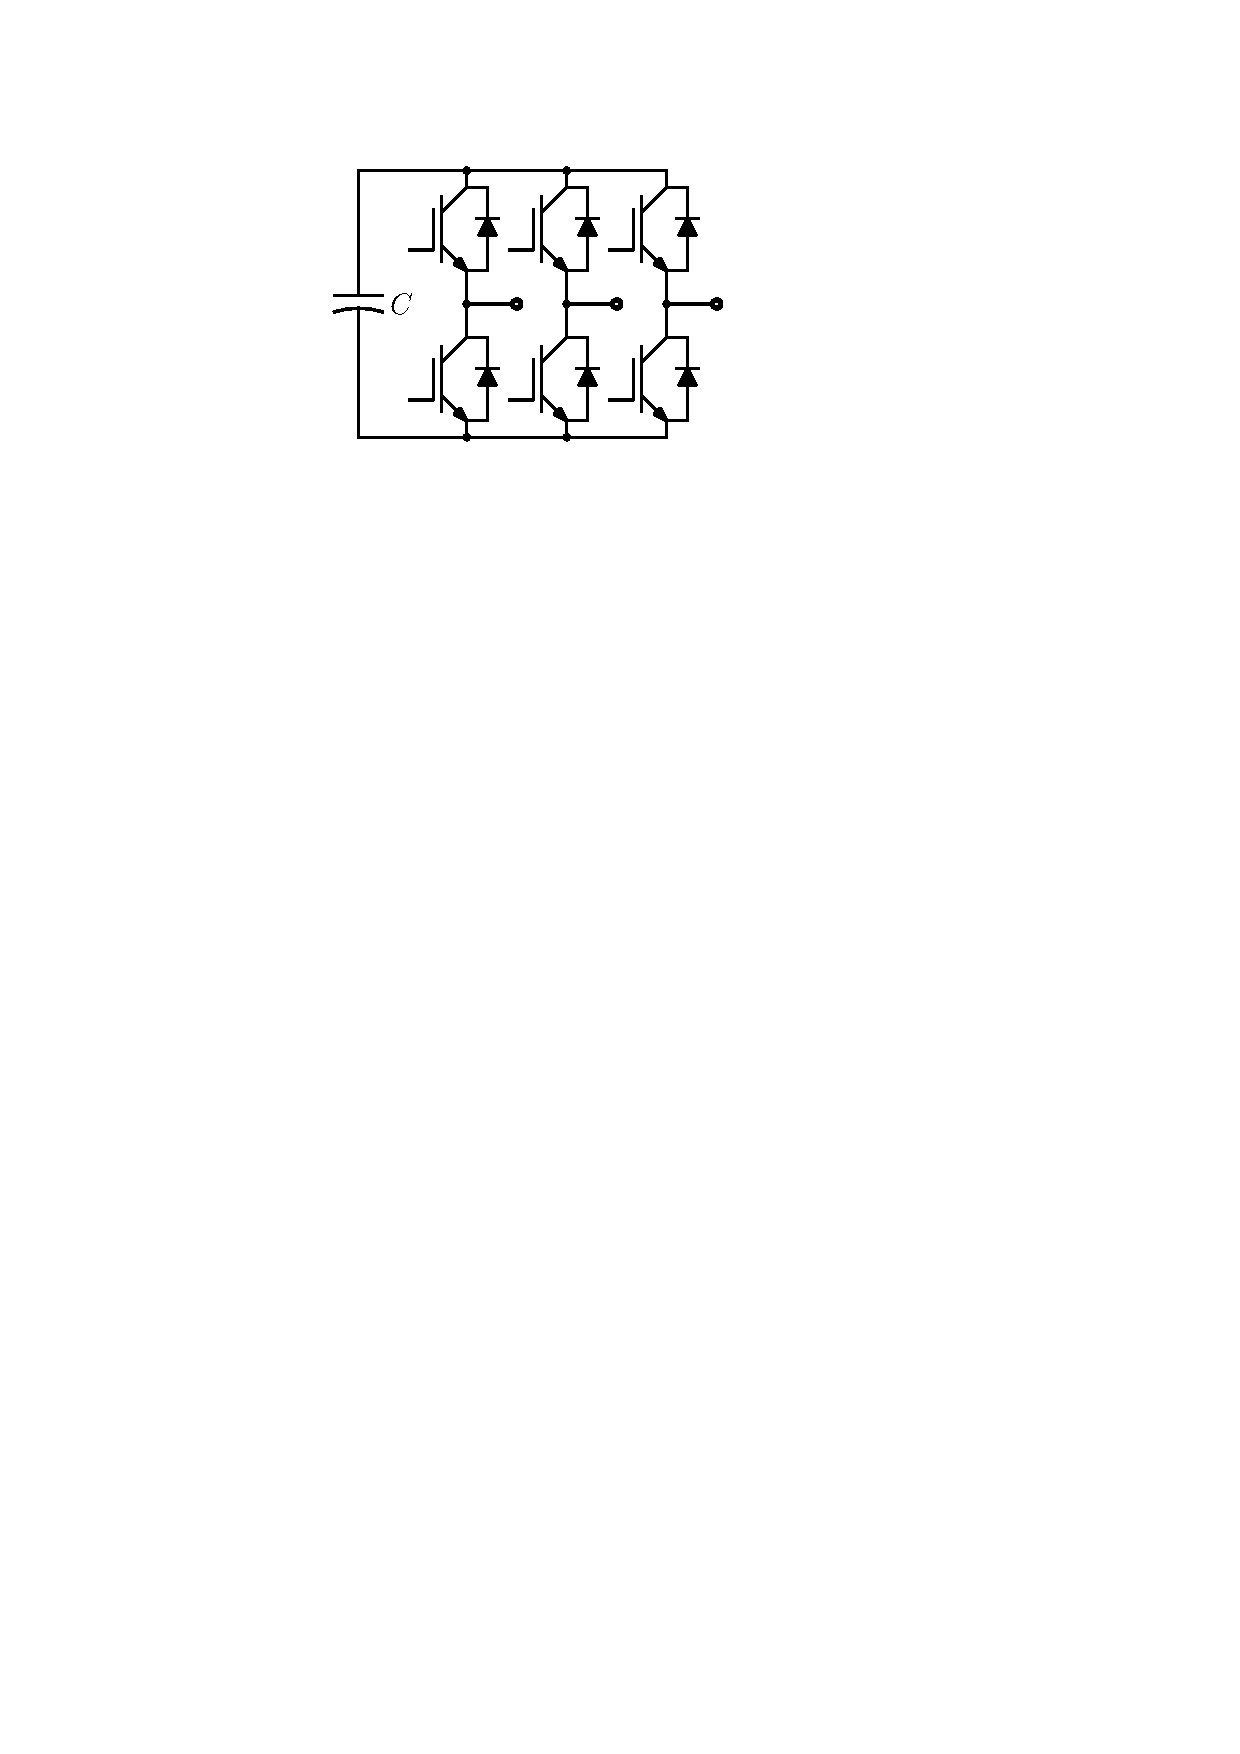
\includegraphics[width=0.8\linewidth]{./figuras/introducao/2niveis}
%
%
%\column{0.5\linewidth}
%
%\begin{itemize}
%	\item Baseados em IGBT\\[15pt]
%	\item Alta frequência de comutação\\[15pt]
%	\item Totalmente controlável\\[15pt]
%	\item Comum na industria\\[15pt]
%	\item {\color{red}Filtros (dependendo da aplicação)}\\[15pt]
%	\item {\color{red}Limitações em alta tensão}
%\end{itemize}
%
%
%
%
%\end{columns}
%
%
%
%
%
%\end{frame}





%%%%%%%%%%%%%%%%%%%%%%%%%%%%%%%%%%%%%%%%%%%%%%%%%%%%%%%
%%%%%%%%%%%%%%%%%%%%%%%%%%%%%%%%%%%%%%%%%%%%%%%%%%%%%%%
%%%%%%%%%%%%%%%%%%%%%%%%%%%%%%%%%%%%%%%%%%%%%%%%%%%%%%%
\begin{frame}{Conversores Fonte de Tensão: Dois Níveis}


\begin{columns}

\column{0.5\linewidth}
\centering

Baixa Tensão\\[20pt]

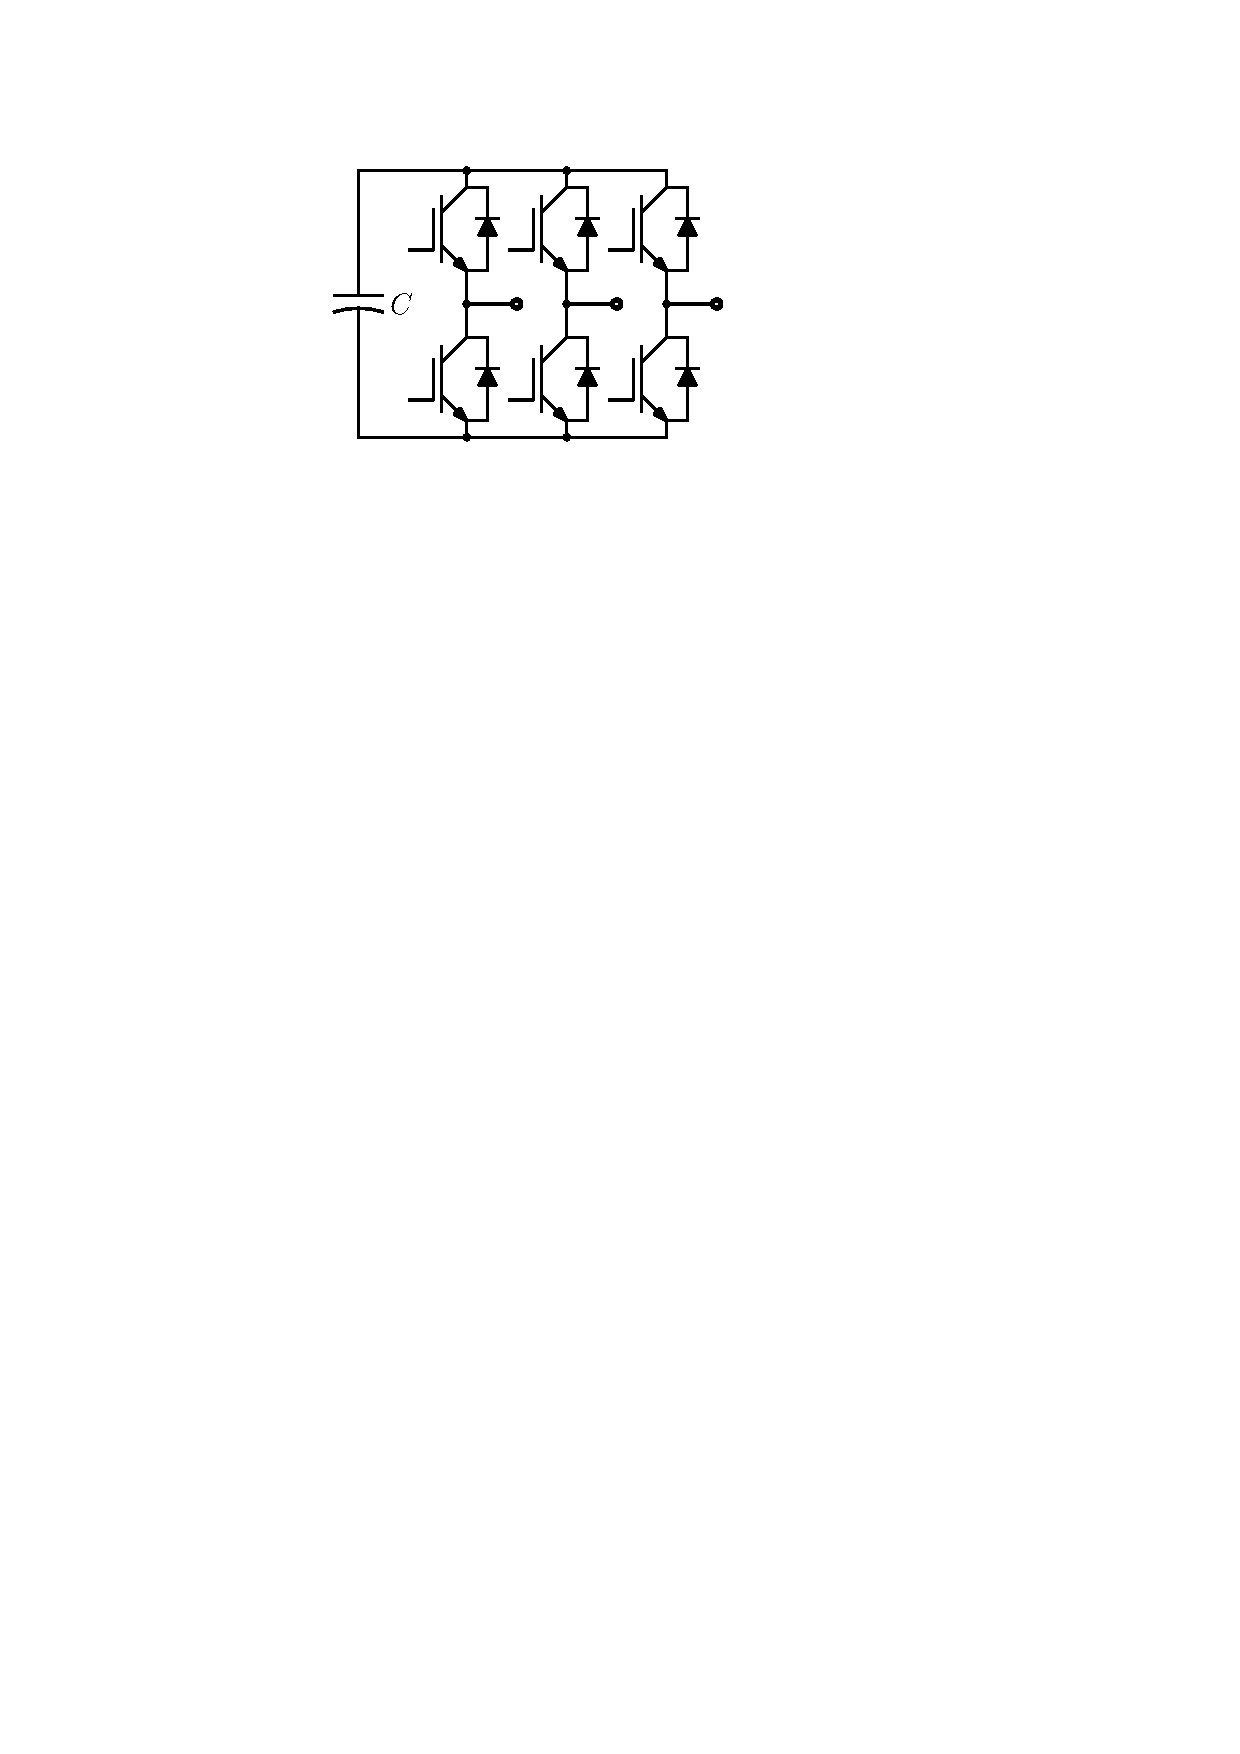
\includegraphics[width=0.6\linewidth]{./figuras/introducao/2niveis}


\column{0.5\linewidth}
\centering


Média e Alta Tensão\\[20pt]

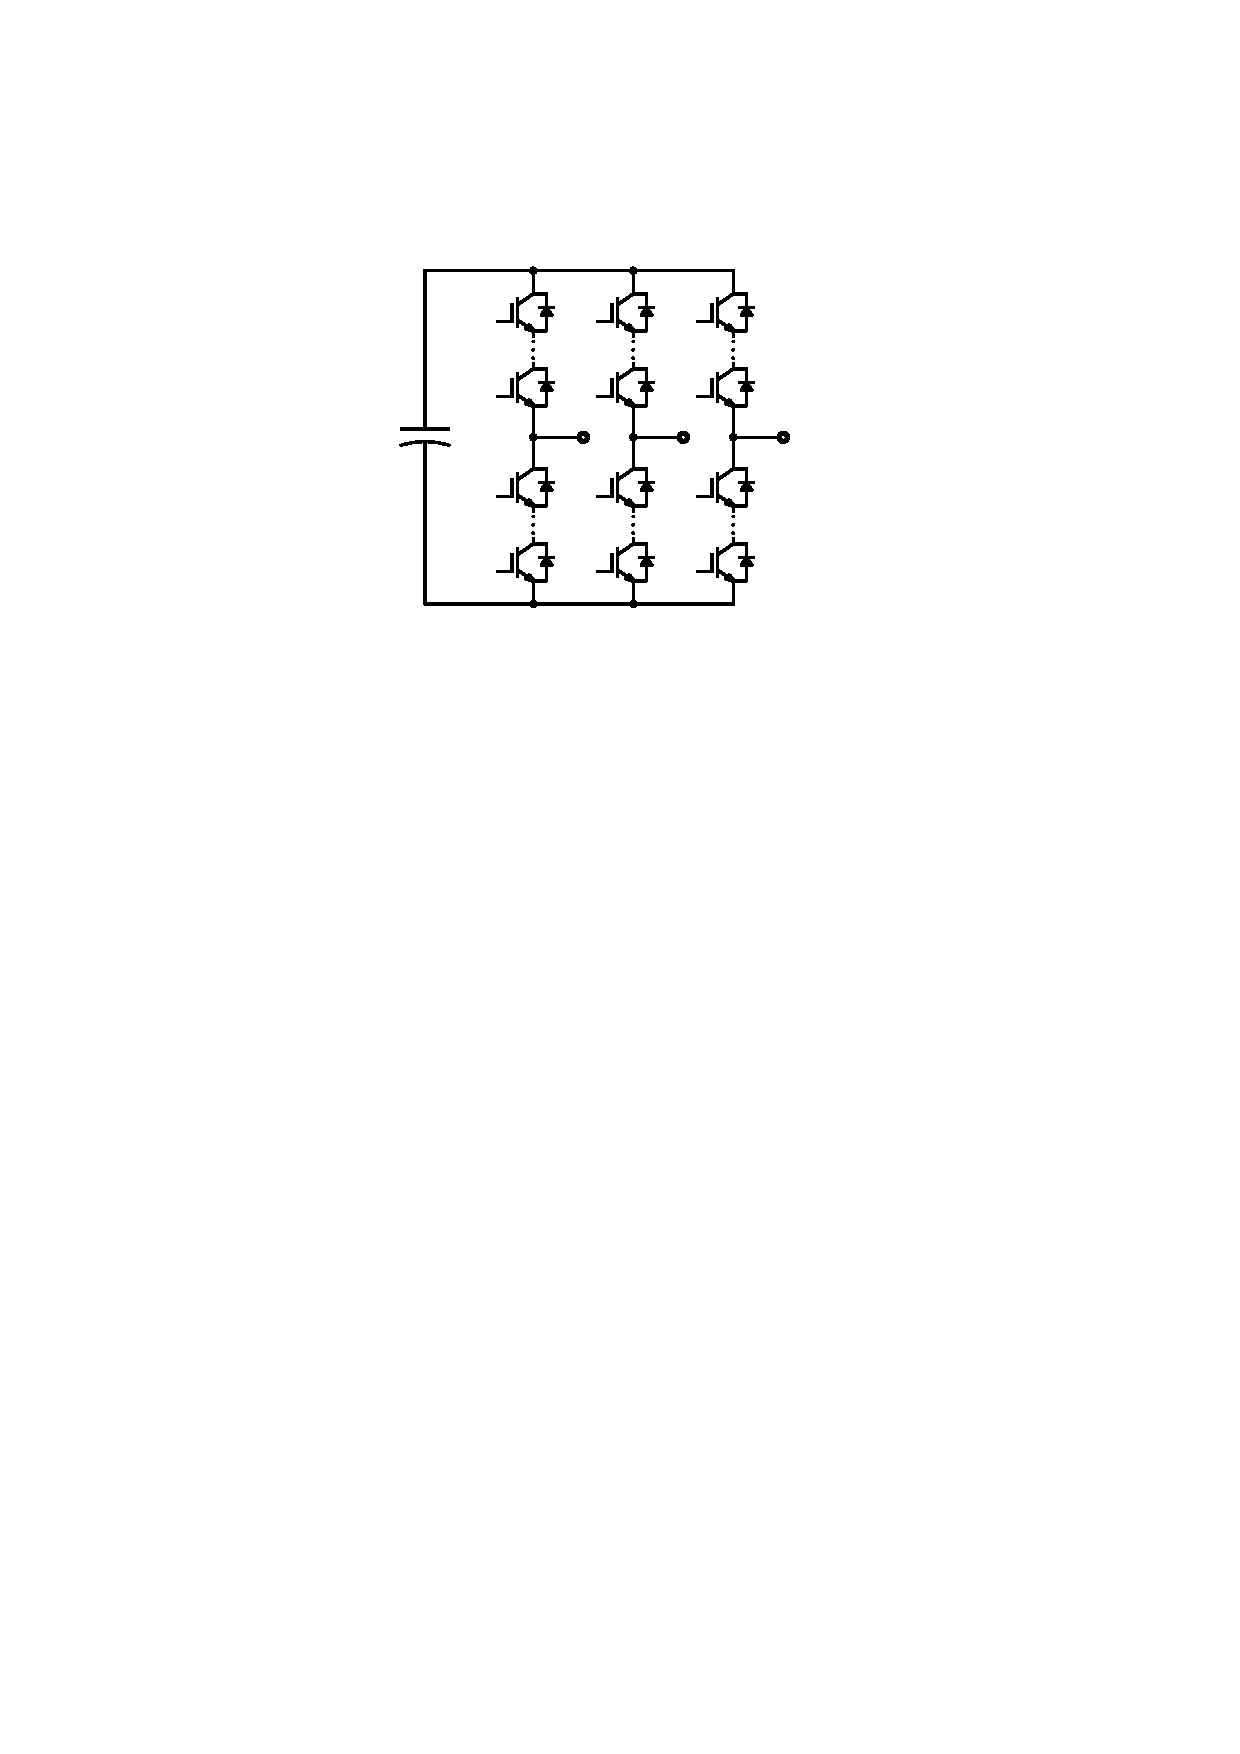
\includegraphics[width=0.55\linewidth]{./figuras/introducao/2niveis_alta}



\end{columns}





\end{frame}



%%%%%%%%%%%%%%%%%%%%%%%%%%%%%%%%%%%%%%%%%%%%%%%%%%%%%%%
%%%%%%%%%%%%%%%%%%%%%%%%%%%%%%%%%%%%%%%%%%%%%%%%%%%%%%%
%%%%%%%%%%%%%%%%%%%%%%%%%%%%%%%%%%%%%%%%%%%%%%%%%%%%%%%
\begin{frame}{Conversor Multinível Modular (MMC)}



\begin{columns}

\column{0.5\textwidth}



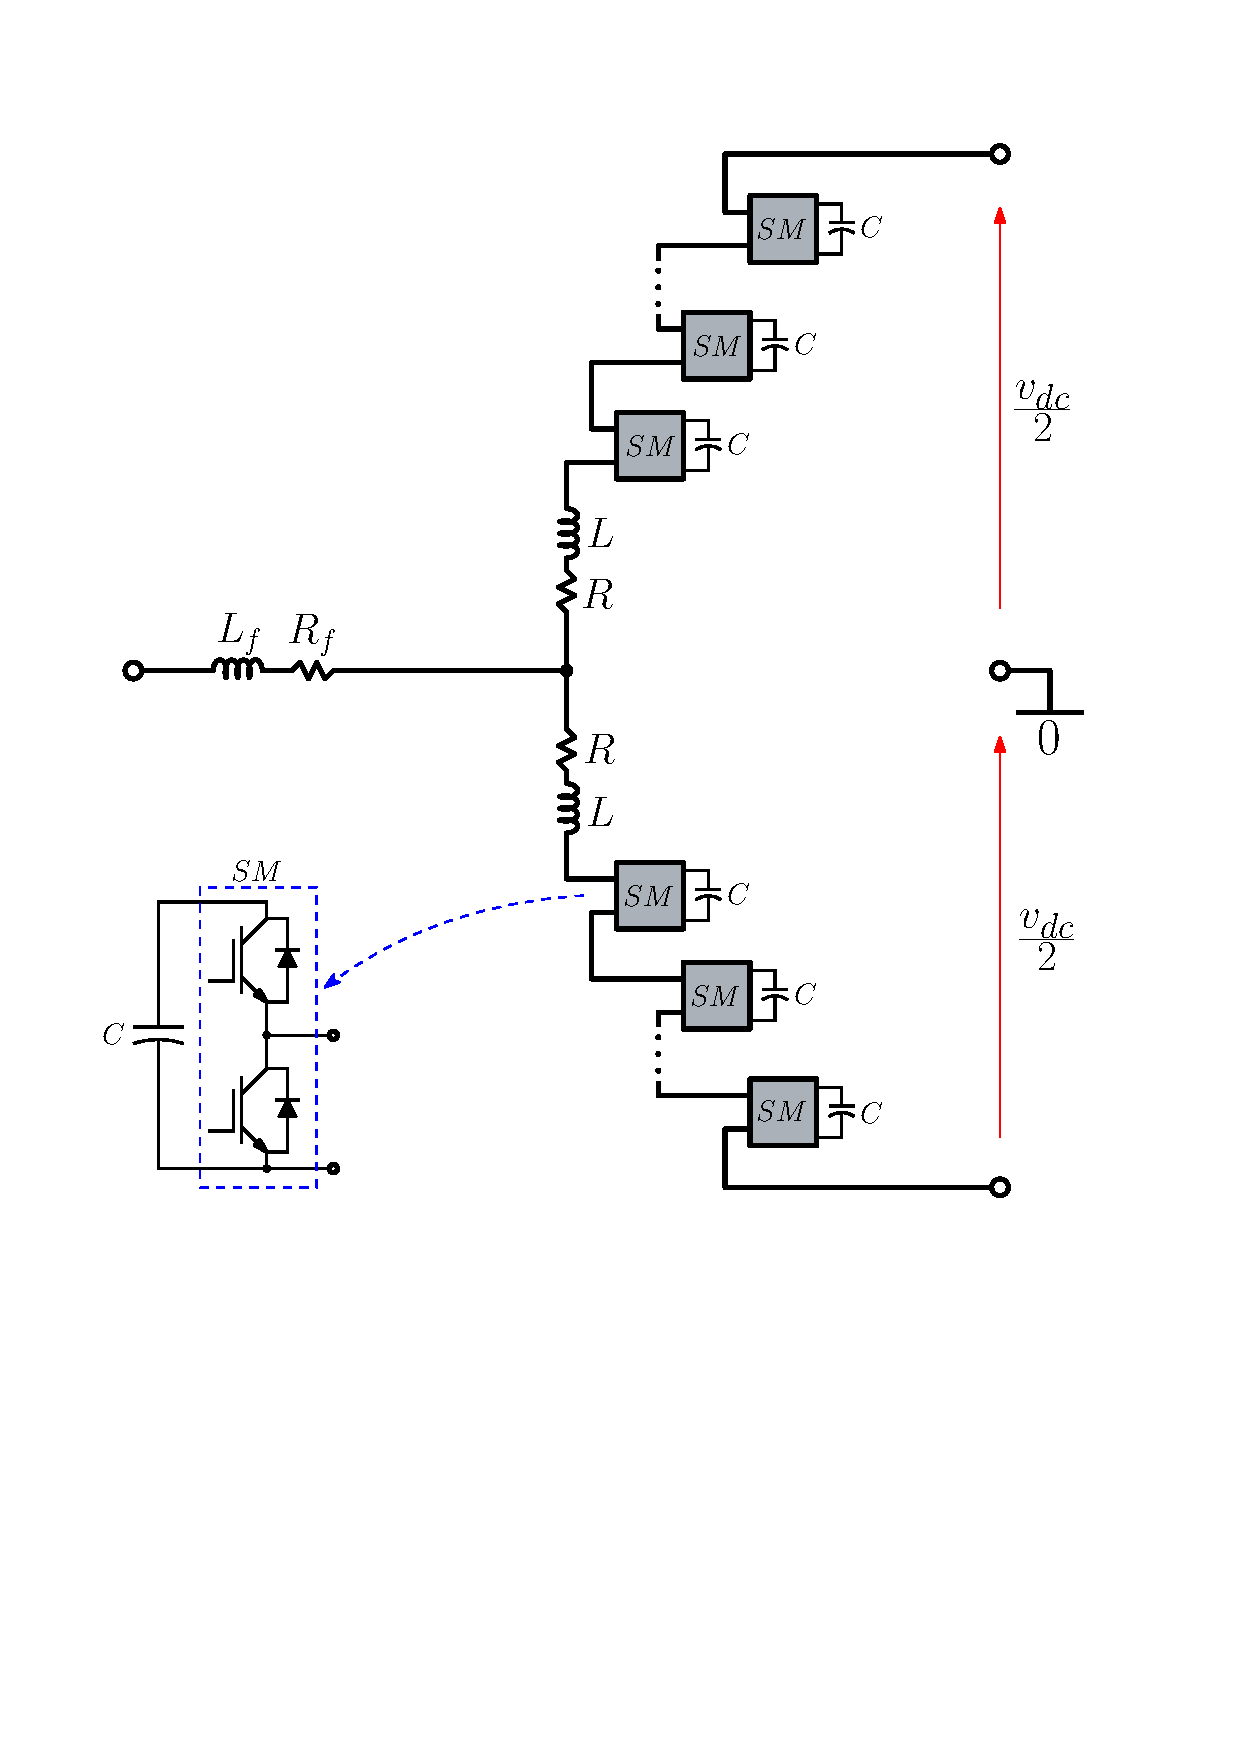
\includegraphics[width=0.9\linewidth]{./figuras/introducao/MMC_blk_limpo}







\column{0.5\textwidth}

%Aplicações

\definecolor{heavy-gray}{rgb}{0.31,0.31,0.31}




\begin{itemize}
	\item Associação de vários submódulos \\[25pt]
	\item Aplicações em alta tensão \\[25pt]
	\item Facilmente escalonável \\[25pt]
	\item {\color{blue}HVDC} \\[25pt]
	\item {\color{blue}FACTs}
\end{itemize}



\end{columns}



\end{frame}









%%%%%%%%%%%%%%%%%%%%%%%%%%%%%%%%%%%%%%%%%%%%%%%%%%%%%%%
%%%%%%%%%%%%%%%%%%%%%%%%%%%%%%%%%%%%%%%%%%%%%%%%%%%%%%%
%%%%%%%%%%%%%%%%%%%%%%%%%%%%%%%%%%%%%%%%%%%%%%%%%%%%%%%
\begin{frame}{Atualidade: Conexão de Usinas Eólicas {\it Offshore}}

\centering

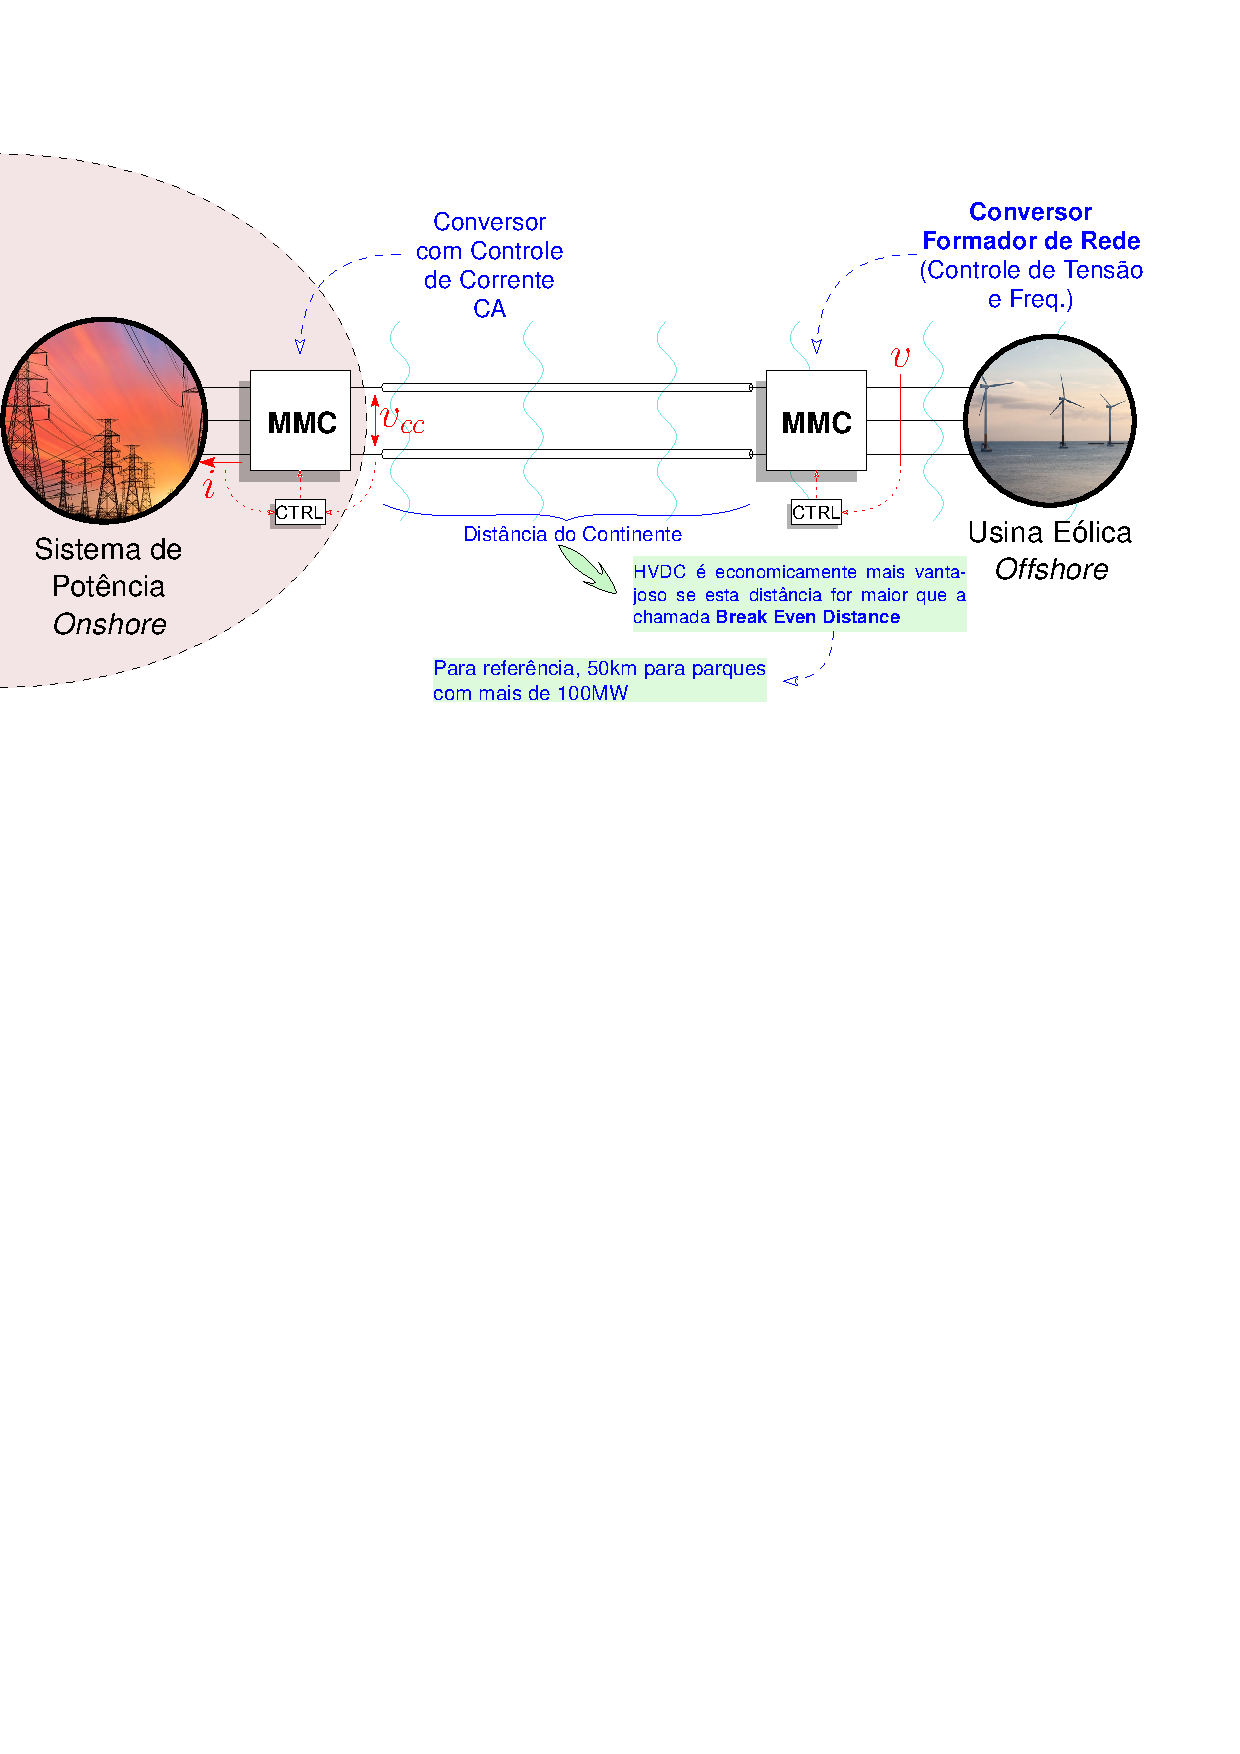
\includegraphics[width=\linewidth]{./figuras/introducao/MMC-HVDC-2}


\end{frame}











%%%%%%%%%%%%%%%%%%%%%%%%%%%%%%%%%%%%%%%%%%%%%%%%%%%%%%%
%%%%%%%%%%%%%%%%%%%%%%%%%%%%%%%%%%%%%%%%%%%%%%%%%%%%%%%
%%%%%%%%%%%%%%%%%%%%%%%%%%%%%%%%%%%%%%%%%%%%%%%%%%%%%%%
\begin{frame}{Foco do Trabalho}



\begin{itemize}
	\item Obter modelos matemáticos analíticos no domínio da frequência considerando diferentes modos de controle: 
	
	\begin{itemize}
		\item Controle por corrente CA
		\item Controle por tensão CA (formador de rede)
		\item Controle em referencial natural
		\item Controle em referencial síncrono
	\end{itemize}

	\item Realizar análises:
	
	\begin{itemize}
		\item Influência dos controladores
		\item Derivações de impedâncias/admitâncias virtuais para melhorar a performance do MMC
	\end{itemize}
	
	\item Apresentar aplicação:
	
	\begin{itemize}
		\item Análise de estabilidade de sistemas baseados em MMC
	\end{itemize}
	
	
\end{itemize}










%Modelos em referencial natural e em referencial síncrono para o MMC formador de rede com malha dupla (corrente e tensão).


%
%\begin{itemize}
%	\item Será focada nos modelos ;
%	
%	\item Considerar um banco capacitivo $C_f$ (...)
%	
%	\item Obter o modelo para a malha de corrente
%	
%	\item Obter um modelo para malha de tensão sem considerar $C_f$
%	
%	\item Incluir $C_f$ no modelo.
%\end{itemize}


\end{frame}






\cmfnewsection{Visão Geral do PSCAD e do Curso}{./logos/fundo_tese}{0.15}






%%%%%%%%%%%%%%%%%%%%%%%%%%%%%%%%%%%%%%%%%%%%%%%%
%%%%%%%%%%%%%%%%%%%%%%%%%%%%%%%%%%%%%%%%%%%%%%%%
%%%%%%%%%%%%%%%%%%%%%%%%%%%%%%%%%%%%%%%%%%%%%%%%
%%%%%%%%%%%%%%%%%%%%%%%%%%%%%%%%%%%%%%%%%%%%%%%%
\begin{frame}{Objetivo}
\centering

\begin{itemize}
\item Aprender a montar simulações de sistemas elétricos no PSCAD 
\vspace*{1cm}
\item Aprender a extrair resultados
\vspace*{1cm}
\item Possivelmente, aprender o funcionamento de alguns circuitos básicos.
\vspace*{1cm}
\end{itemize}

\end{frame}






%%%%%%%%%%%%%%%%%%%%%%%%%%%%%%%%%%%%%%%%%%%%%%%%
%%%%%%%%%%%%%%%%%%%%%%%%%%%%%%%%%%%%%%%%%%%%%%%%
%%%%%%%%%%%%%%%%%%%%%%%%%%%%%%%%%%%%%%%%%%%%%%%%
%%%%%%%%%%%%%%%%%%%%%%%%%%%%%%%%%%%%%%%%%%%%%%%%
\begin{frame}{O que é o PSCAD}
\centering

\begin{itemize}
\item O PSCAD ({\it Power Systems Computer Aided Design}) é uma interface gráfica para simulação no EMTDC

\vspace*{2cm}

\item o EMTDC é um programa utilizado para simulação de transitórios eletromagnéticos.
\end{itemize}

\end{frame}





%%%%%%%%%%%%%%%%%%%%%%%%%%%%%%%%%%%%%%%%%%%%%%%%
%%%%%%%%%%%%%%%%%%%%%%%%%%%%%%%%%%%%%%%%%%%%%%%%
%%%%%%%%%%%%%%%%%%%%%%%%%%%%%%%%%%%%%%%%%%%%%%%%
%%%%%%%%%%%%%%%%%%%%%%%%%%%%%%%%%%%%%%%%%%%%%%%%
\begin{frame}{Para que serve o PSCAD}
\centering

\begin{itemize}
\item Simulação de sistemas de potência: transitórios eletromagnéticos

\begin{itemize}
\item Redes de distribuição e transmissão
\item Máquinas Elétricas
\item Sistemas de controle de fontes de energia
\end{itemize}

\vspace*{1cm}

\item Simulação de sistemas envolvendo eletrônica de potência.

\begin{itemize}
\item Grid-connected/Grid-Forming Converters
\item HVDCs ({\it High Voltage Direct Current})
\item FACTS ({\it flexible alternating current transmission system})
\item Sistemas de controle
\end{itemize}

\end{itemize}

\end{frame}





%%%%%%%%%%%%%%%%%%%%%%%%%%%%%%%%%%%%%%%%%%%%%%%%
%%%%%%%%%%%%%%%%%%%%%%%%%%%%%%%%%%%%%%%%%%%%%%%%
%%%%%%%%%%%%%%%%%%%%%%%%%%%%%%%%%%%%%%%%%%%%%%%%
%%%%%%%%%%%%%%%%%%%%%%%%%%%%%%%%%%%%%%%%%%%%%%%%
\begin{frame}{Ideia Geral do PSCAD}
\centering


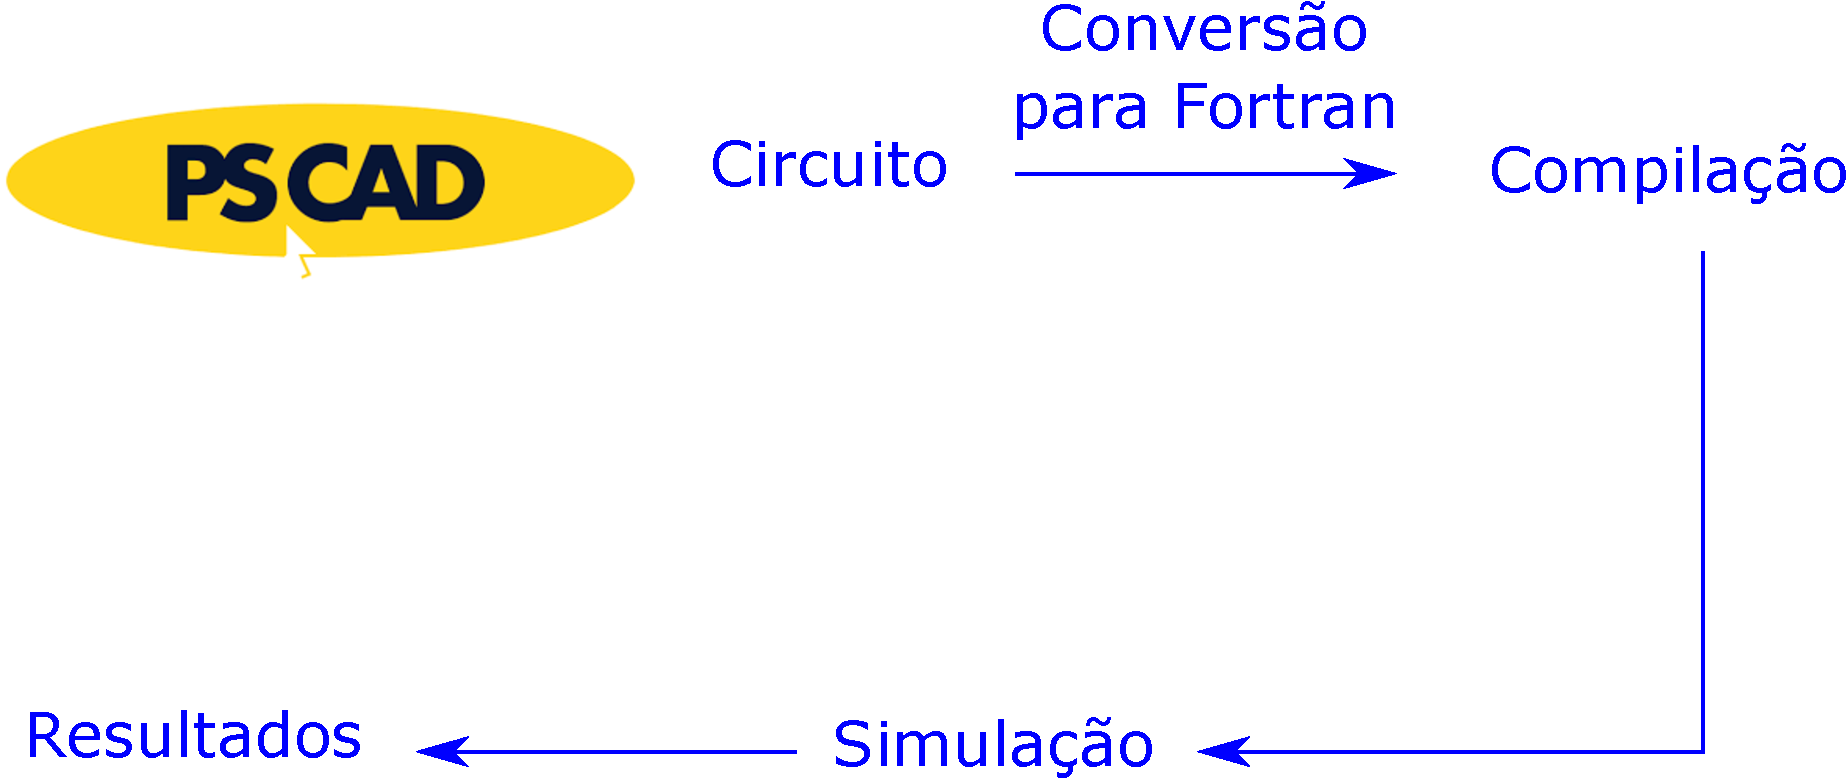
\includegraphics[width=0.95\linewidth]{./figuras/geral/fluxo}

\end{frame}

\cmfnewsection{Primeiros Passos no PSCAD}{./logos/fundo_tese}{0.15}





%%%%%%%%%%%%%%%%%%%%%%%%%%%%%%%%%%%%%%%%%%%%%%%%
%%%%%%%%%%%%%%%%%%%%%%%%%%%%%%%%%%%%%%%%%%%%%%%%
%%%%%%%%%%%%%%%%%%%%%%%%%%%%%%%%%%%%%%%%%%%%%%%%
%%%%%%%%%%%%%%%%%%%%%%%%%%%%%%%%%%%%%%%%%%%%%%%%
\begin{frame}{PSCAD: Versão Gratuita}
\centering

\begin{columns}
\column{0.3\linewidth}
apenas um teste

\column{0.7\linewidth}
\centering
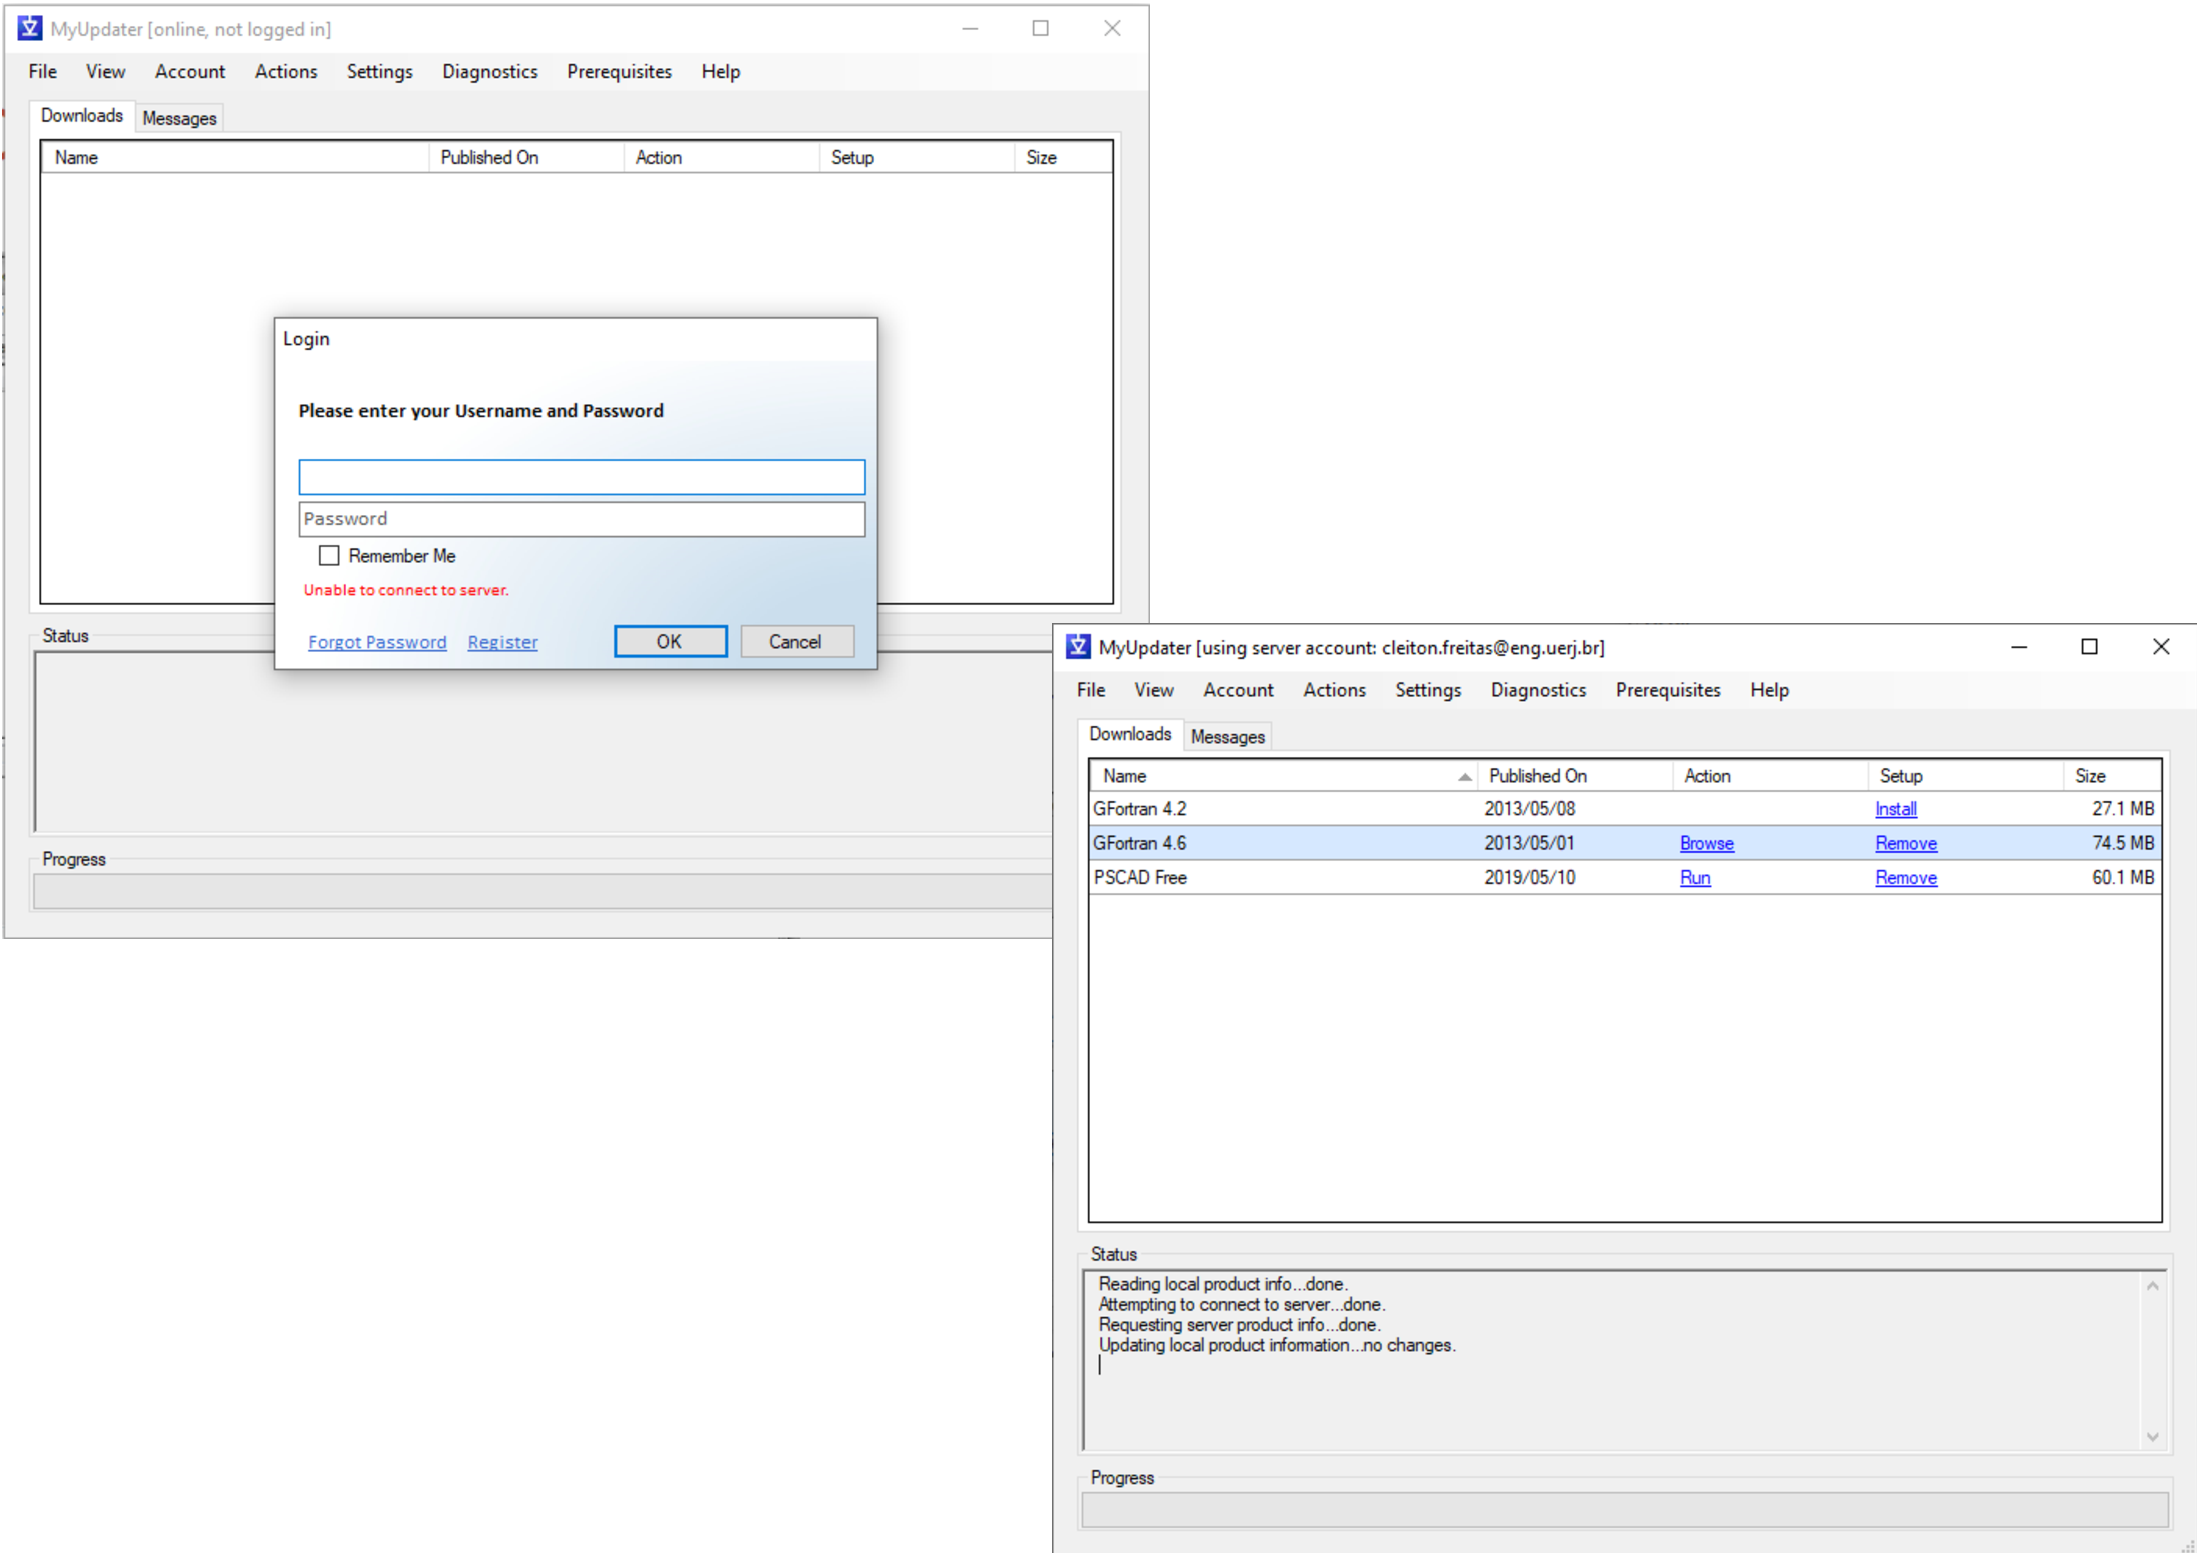
\includegraphics[width=0.8\linewidth]{./figuras/Primeiros-Passos/login}

\end{columns}

\end{frame}


%%%%%%%%%%%%%%%%%%%%%%%%%%%%%%%%%%%%%%%%%%%%%%%%
%%%%%%%%%%%%%%%%%%%%%%%%%%%%%%%%%%%%%%%%%%%%%%%%
%%%%%%%%%%%%%%%%%%%%%%%%%%%%%%%%%%%%%%%%%%%%%%%%
%%%%%%%%%%%%%%%%%%%%%%%%%%%%%%%%%%%%%%%%%%%%%%%%
\begin{frame}{PSCAD: Versão Gratuita}
\centering


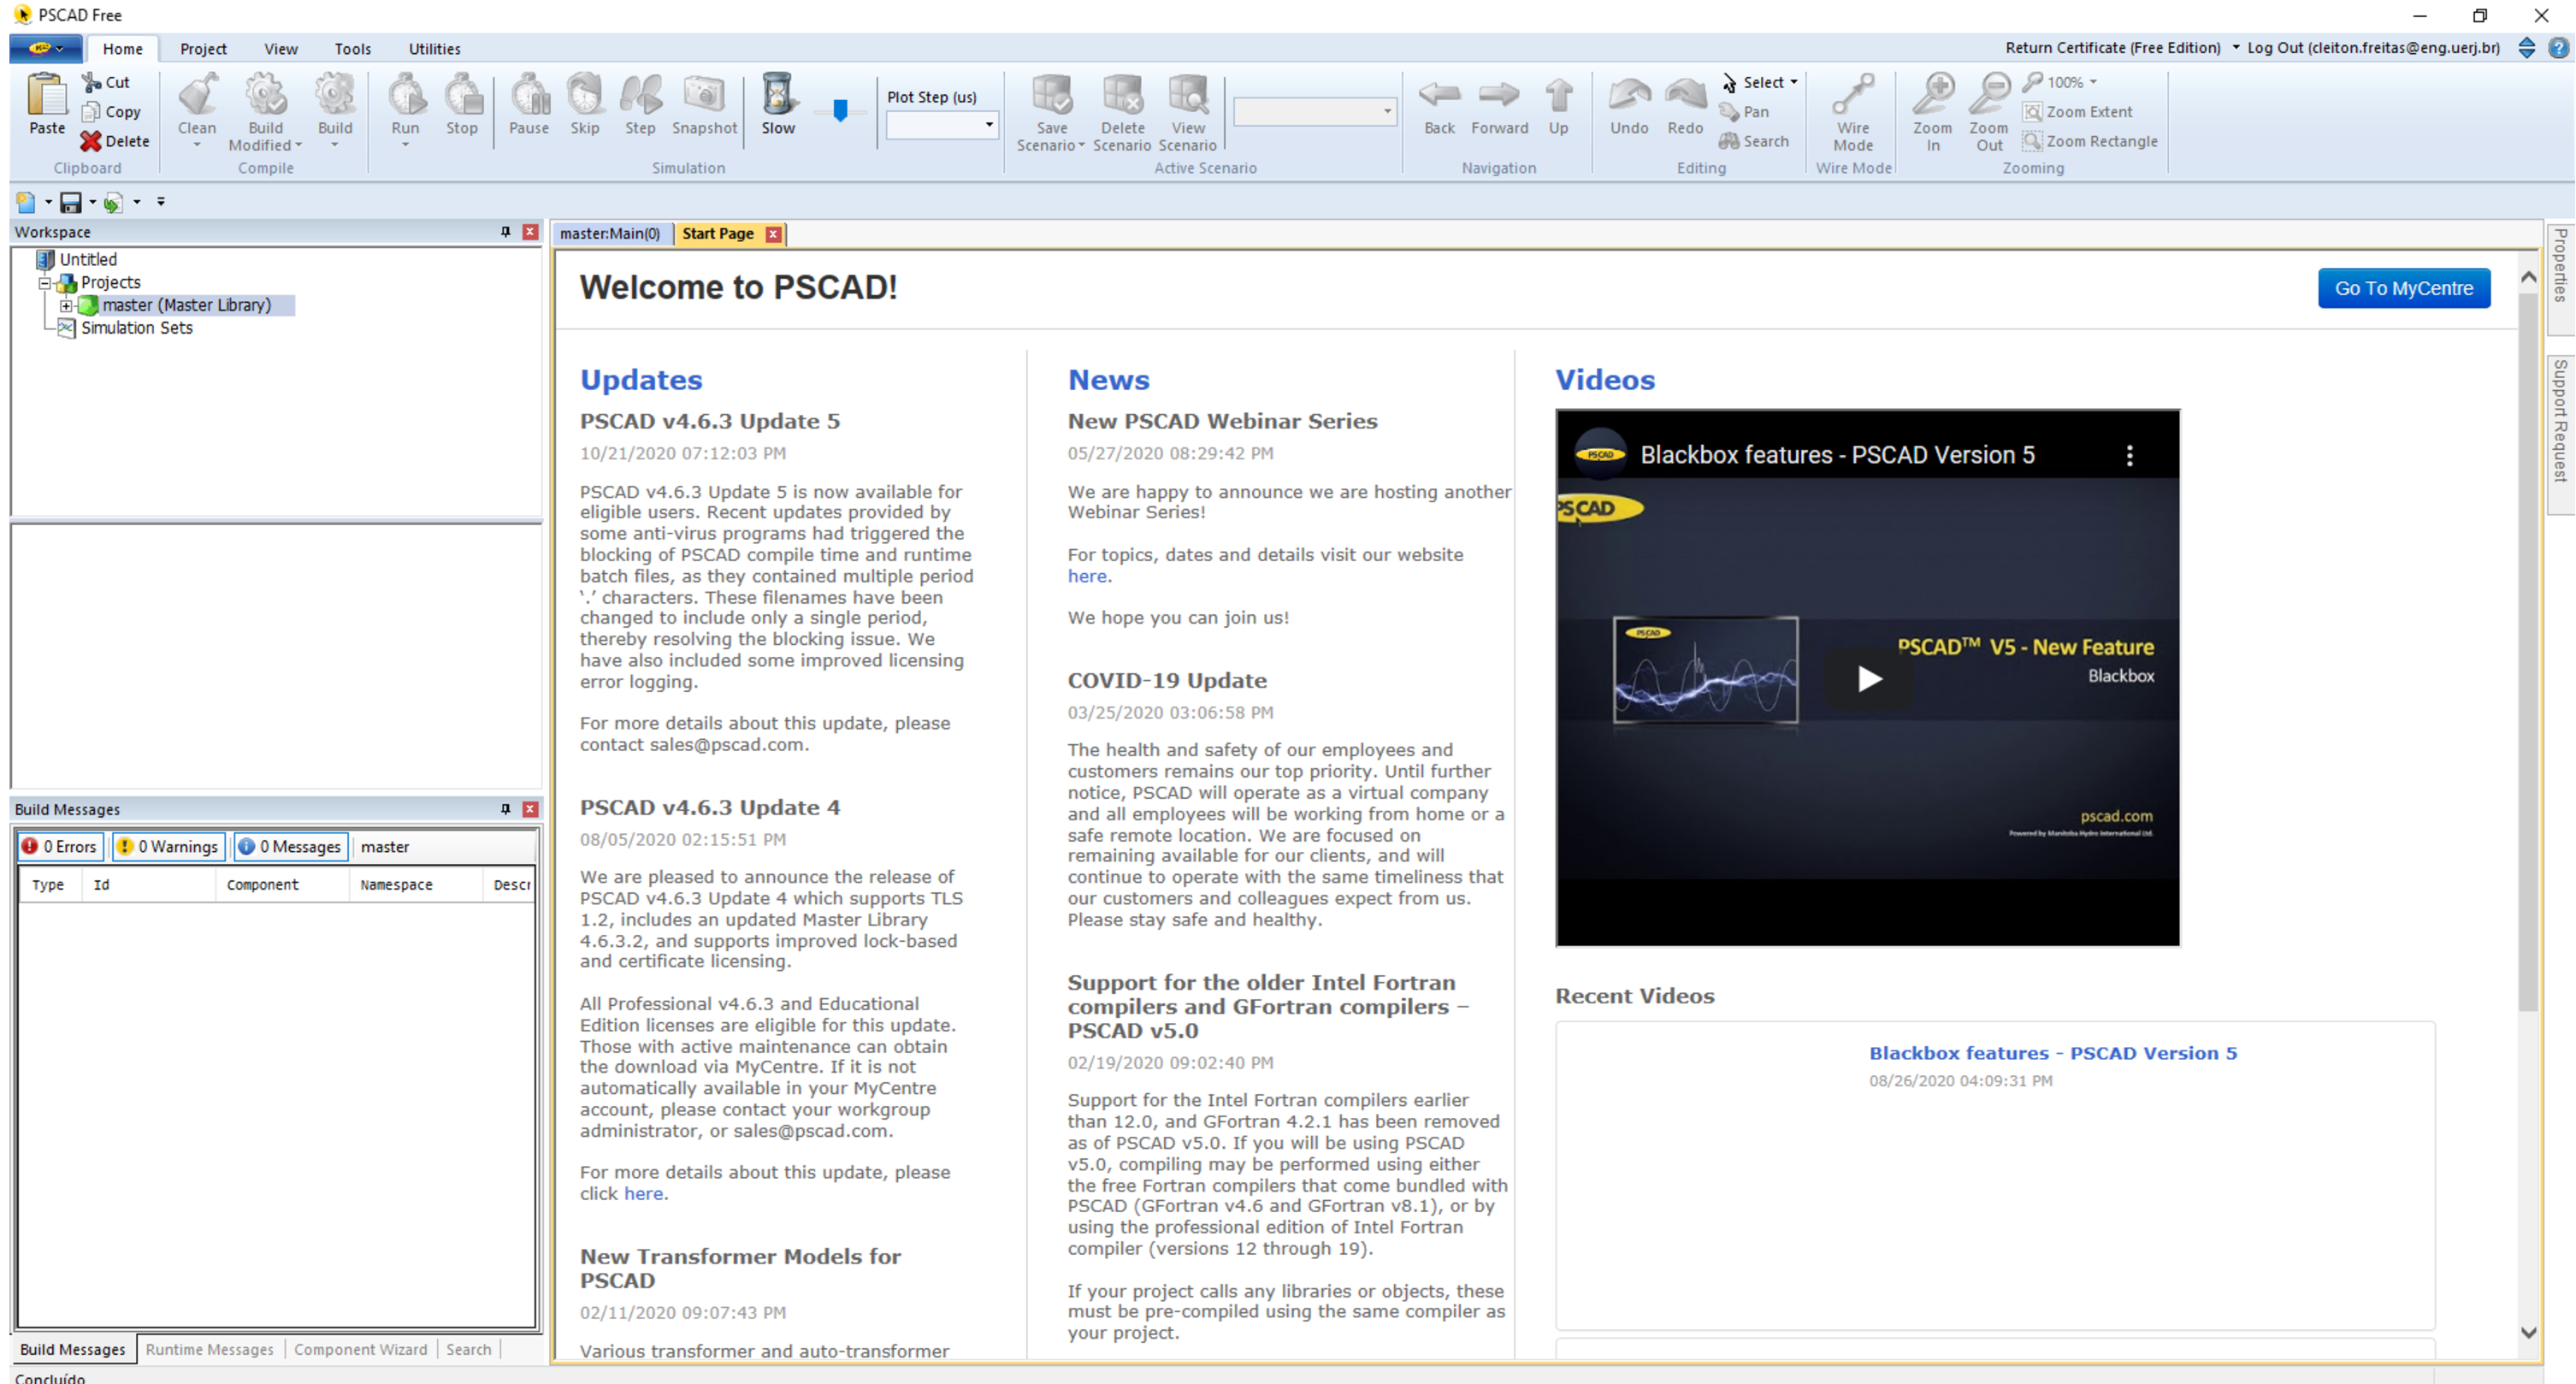
\includegraphics[width=0.85\linewidth]{./figuras/Primeiros-Passos/tela_inicial}


\end{frame}





%%%%%%%%%%%%%%%%%%%%%%%%%%%%%%%%%%%%%%%%%%%%%%%%
%%%%%%%%%%%%%%%%%%%%%%%%%%%%%%%%%%%%%%%%%%%%%%%%
%%%%%%%%%%%%%%%%%%%%%%%%%%%%%%%%%%%%%%%%%%%%%%%%
%%%%%%%%%%%%%%%%%%%%%%%%%%%%%%%%%%%%%%%%%%%%%%%%
\begin{frame}{PSCAD: Biblioteca Master}
\centering


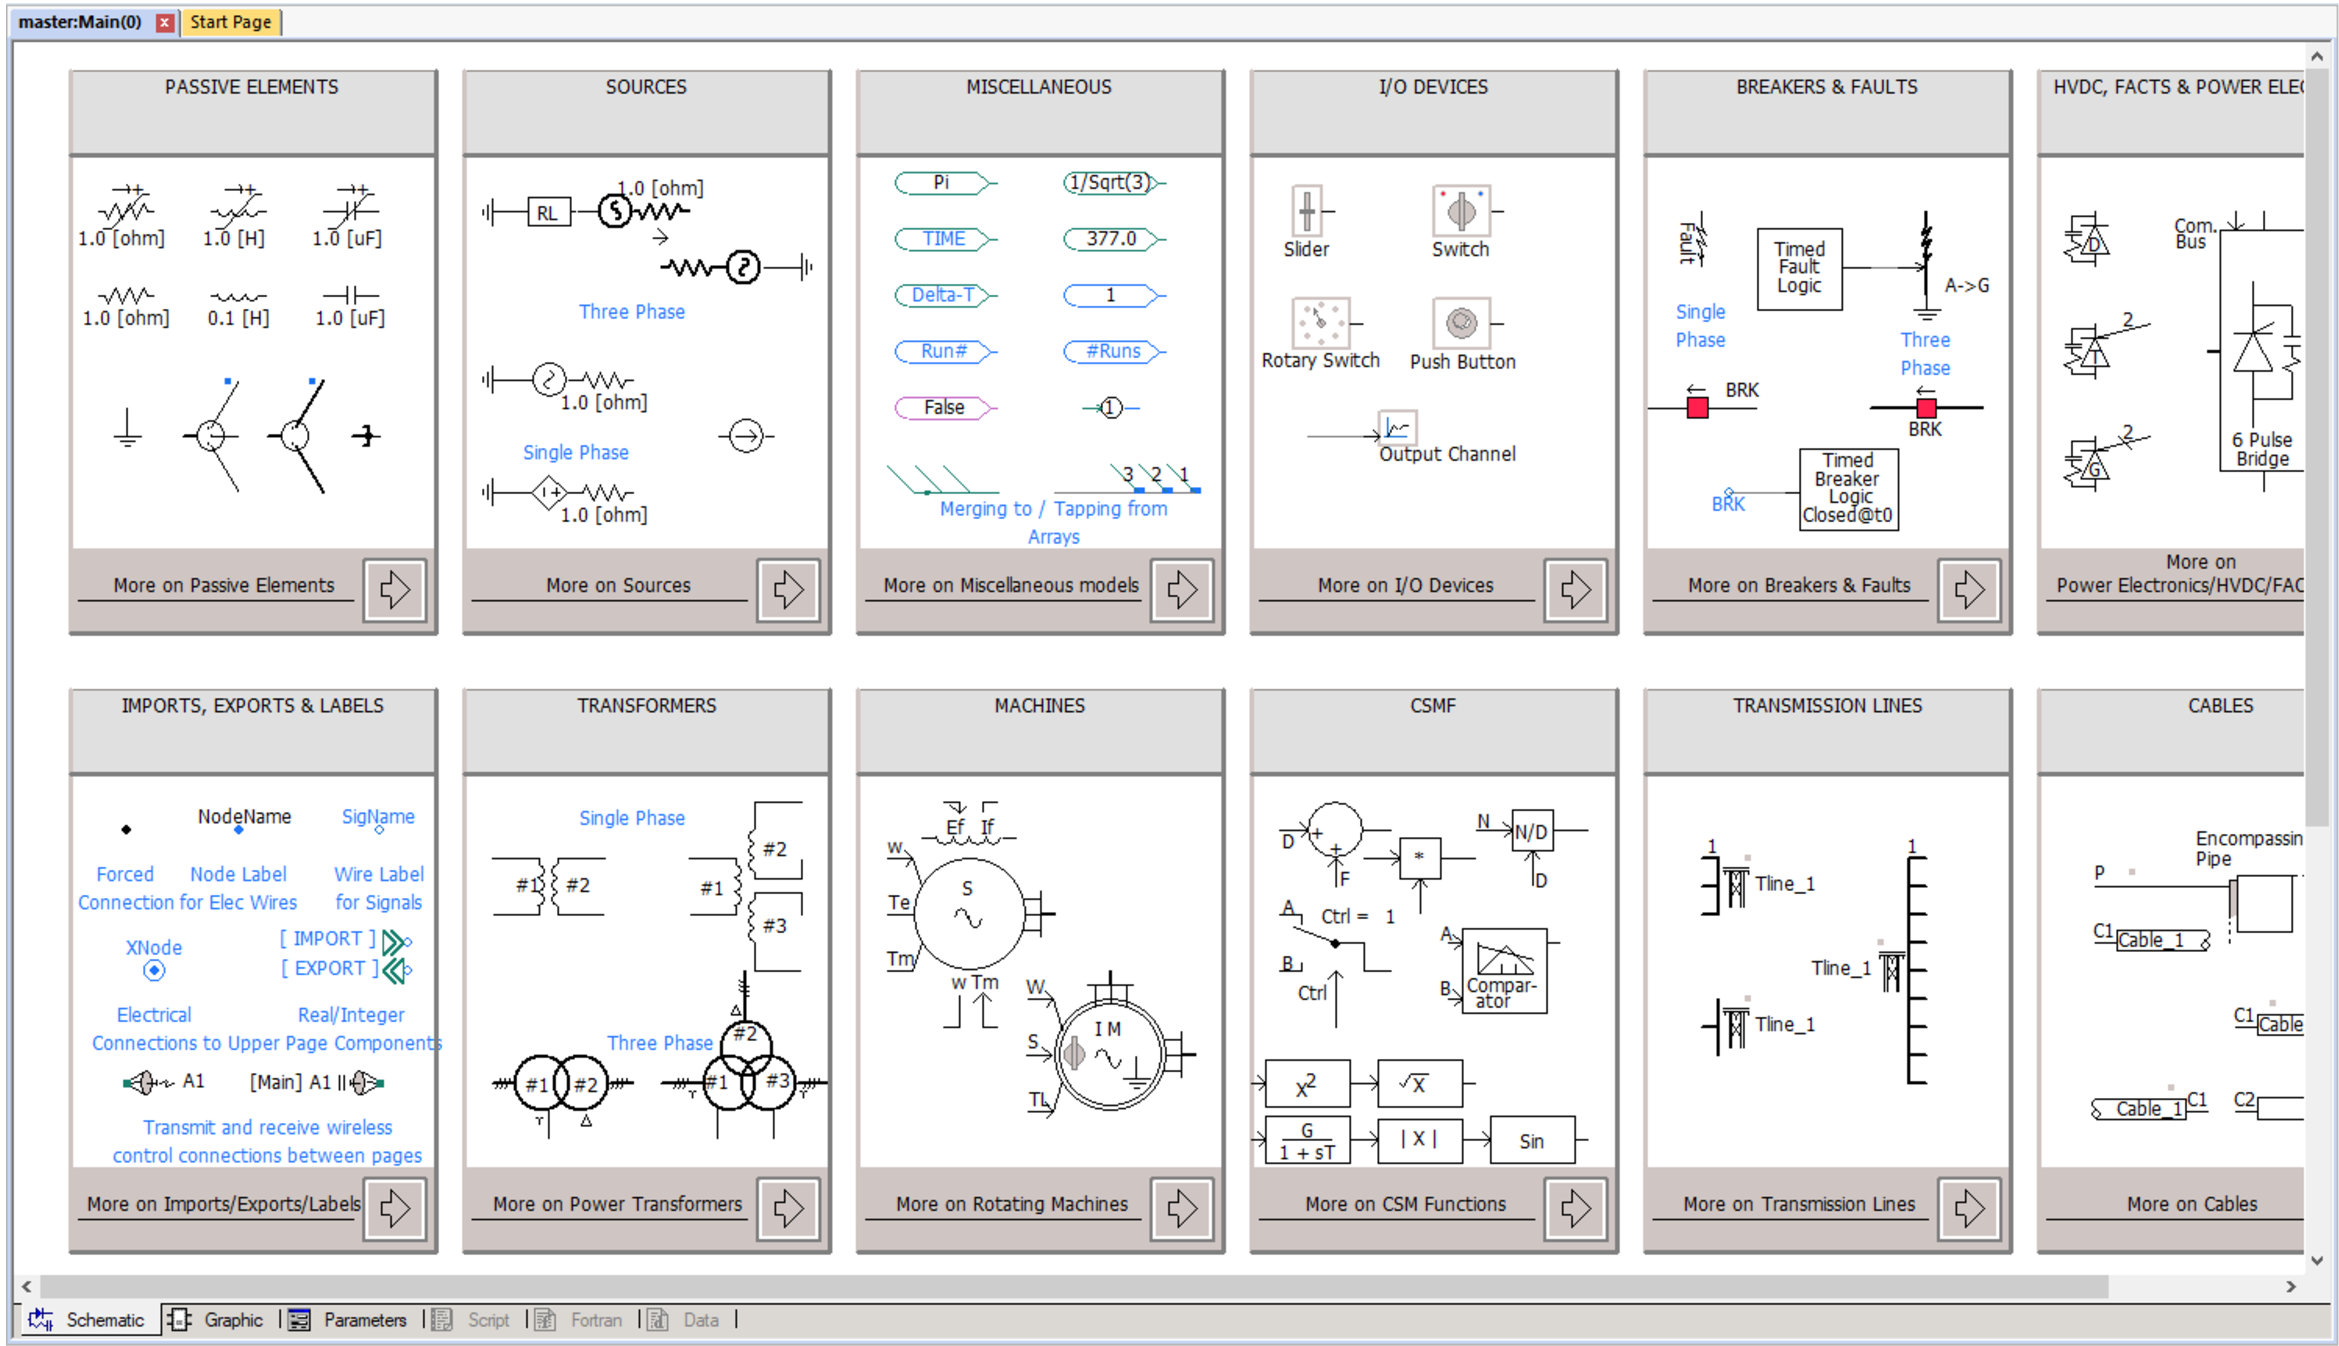
\includegraphics[width=0.85\linewidth]{./figuras/Primeiros-Passos/biblioteca_master}


\end{frame}




%%%%%%%%%%%%%%%%%%%%%%%%%%%%%%%%%%%%%%%%%%%%%%%%
%%%%%%%%%%%%%%%%%%%%%%%%%%%%%%%%%%%%%%%%%%%%%%%%
%%%%%%%%%%%%%%%%%%%%%%%%%%%%%%%%%%%%%%%%%%%%%%%%
%%%%%%%%%%%%%%%%%%%%%%%%%%%%%%%%%%%%%%%%%%%%%%%%
\begin{frame}{PSCAD: Biblioteca Master}
\centering


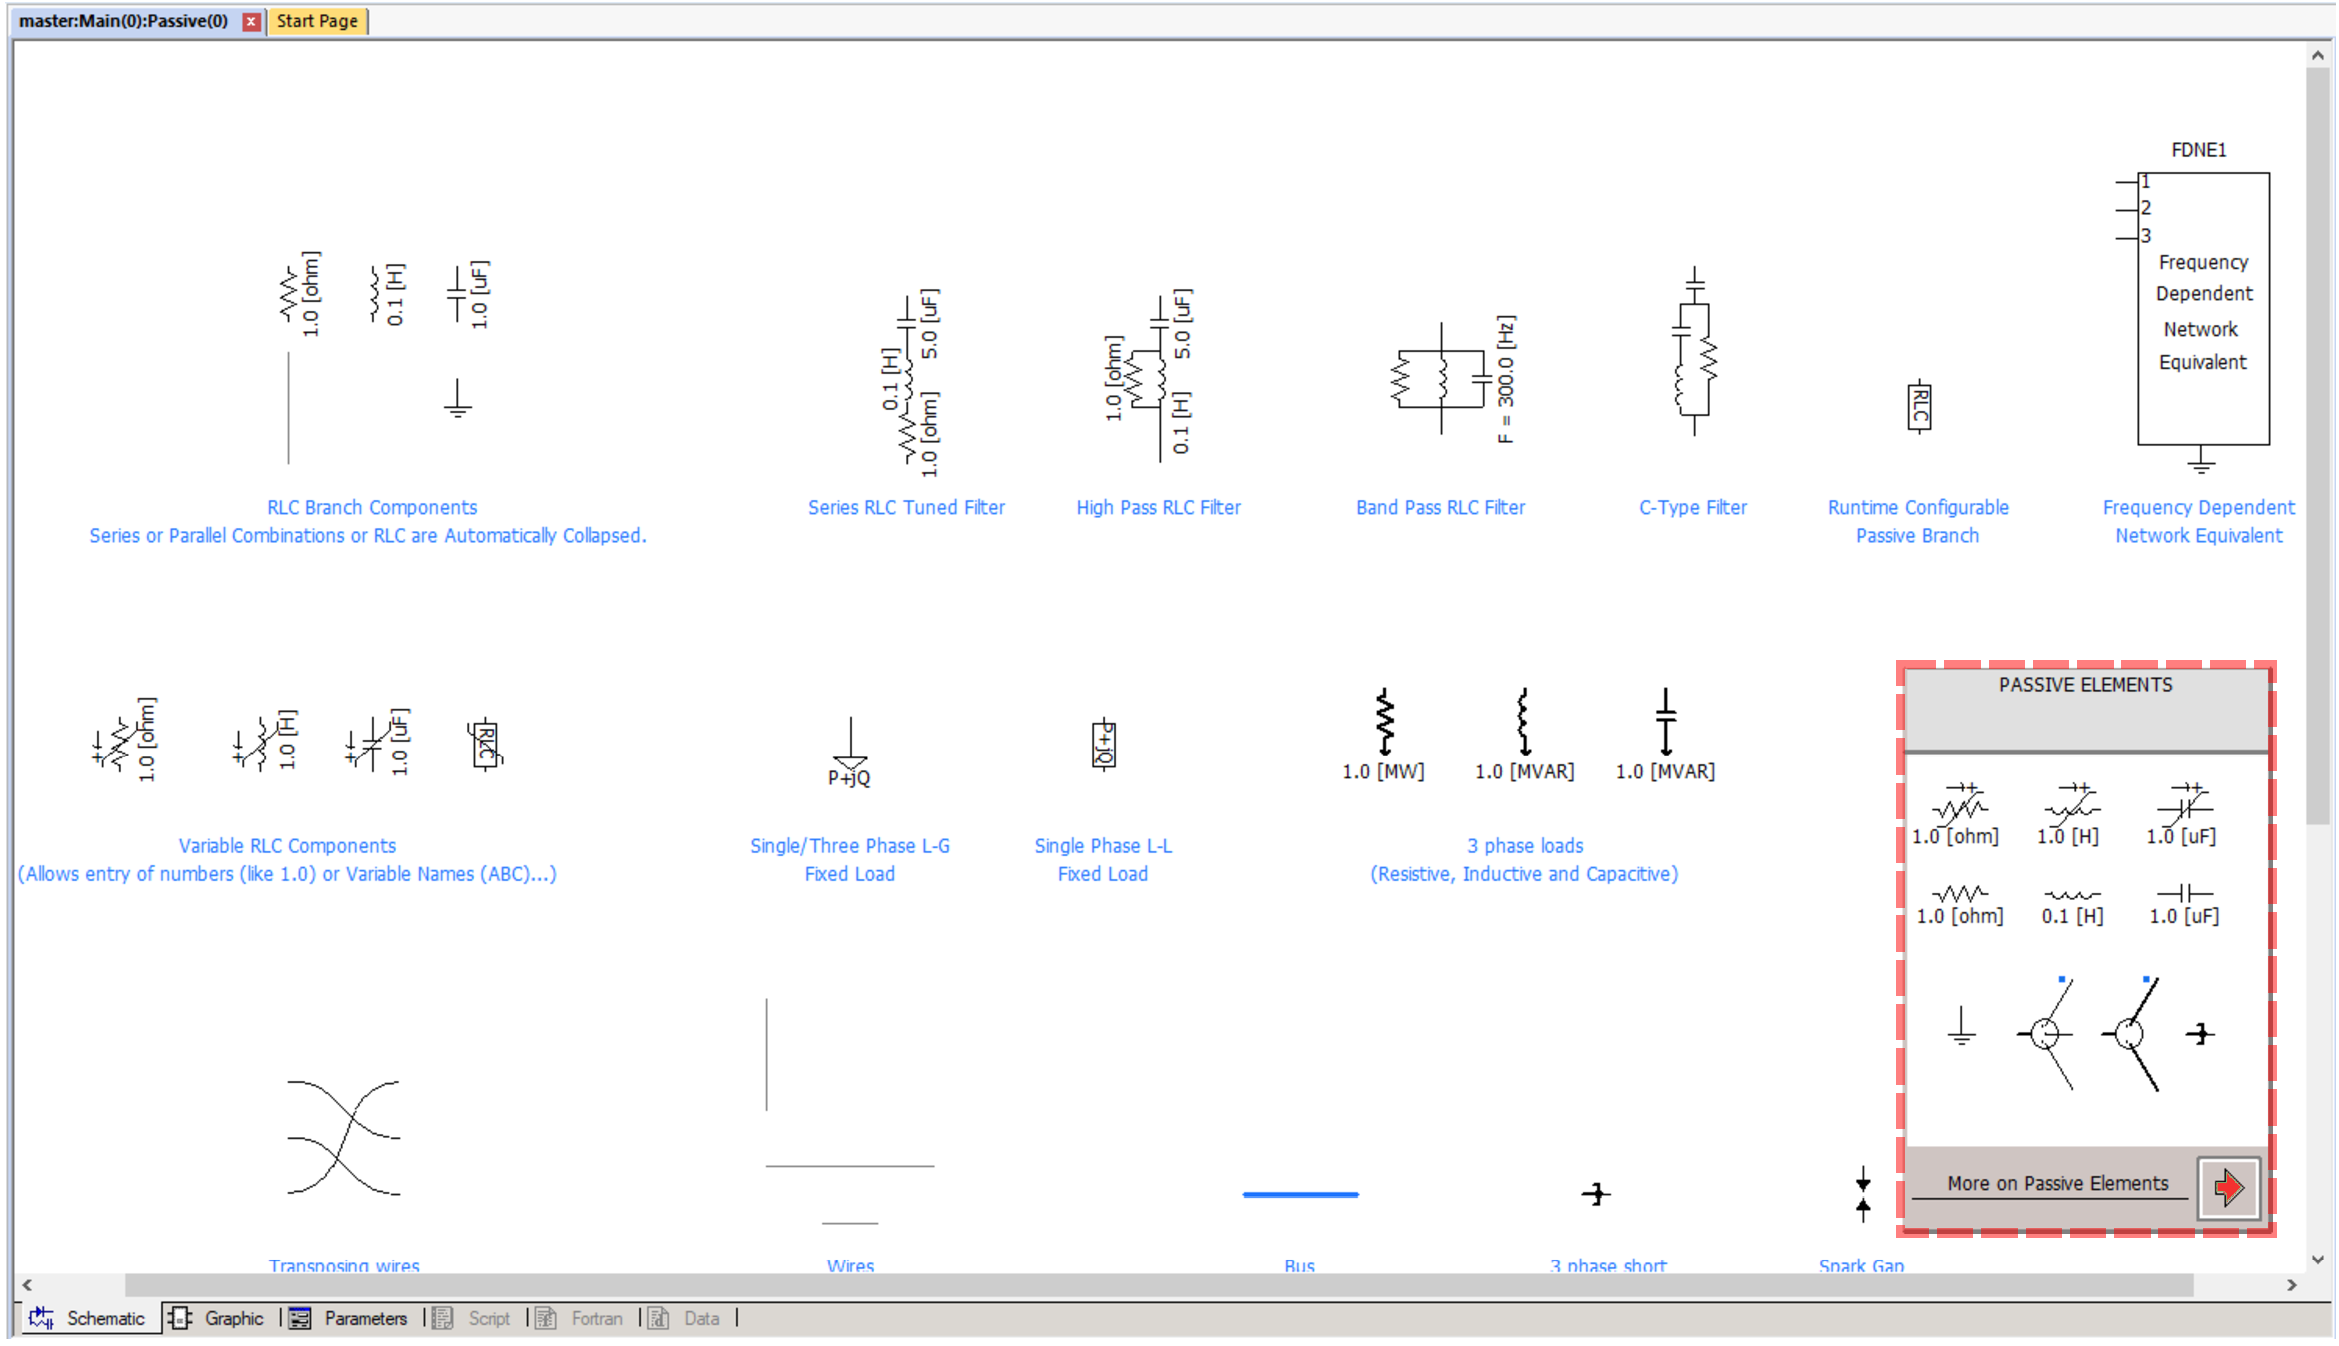
\includegraphics[width=0.85\linewidth]{./figuras/Primeiros-Passos/biblioteca_parte}


\end{frame}





%%%%%%%%%%%%%%%%%%%%%%%%%%%%%%%%%%%%%%%%%%%%%%%%
%%%%%%%%%%%%%%%%%%%%%%%%%%%%%%%%%%%%%%%%%%%%%%%%
%%%%%%%%%%%%%%%%%%%%%%%%%%%%%%%%%%%%%%%%%%%%%%%%
%%%%%%%%%%%%%%%%%%%%%%%%%%%%%%%%%%%%%%%%%%%%%%%%
\begin{frame}{PSCAD: Biblioteca Master}
\centering


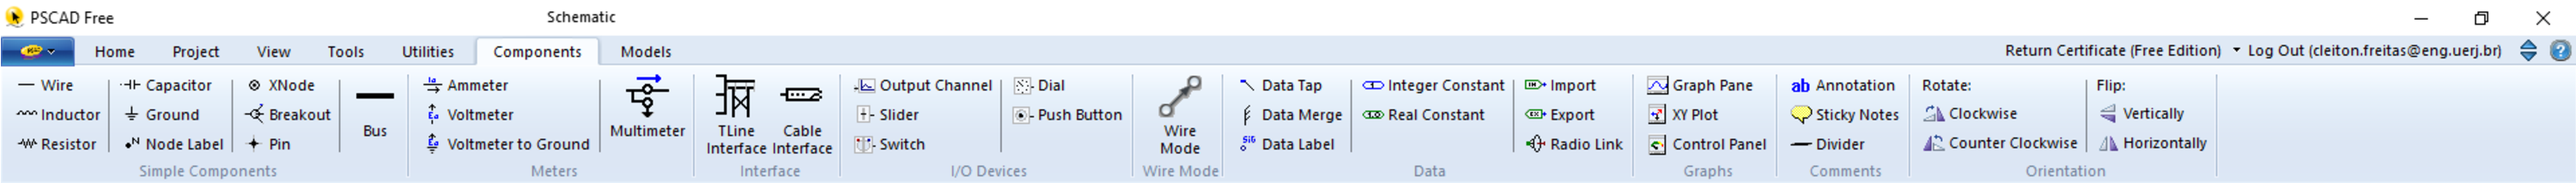
\includegraphics[width=0.85\linewidth]{./figuras/Primeiros-Passos/biblioteca_barra_components}
\vspace*{1cm}

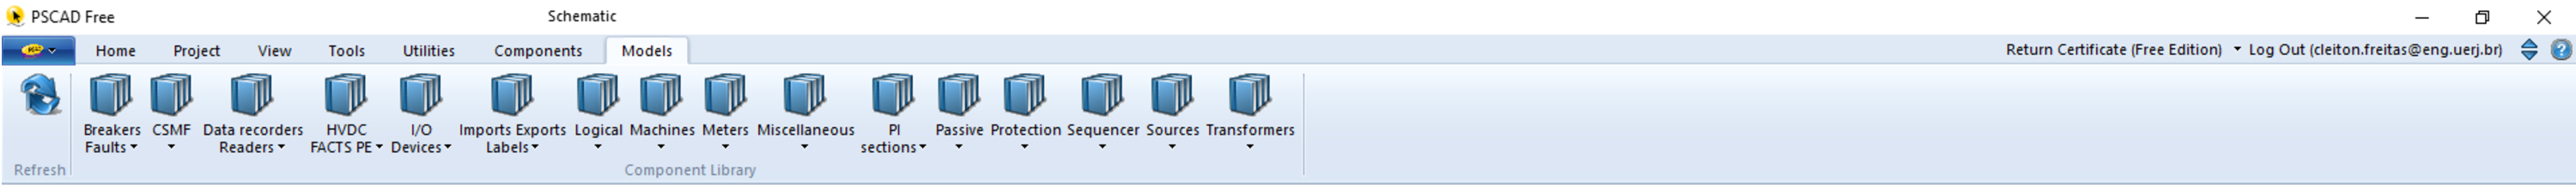
\includegraphics[width=0.85\linewidth]{./figuras/Primeiros-Passos/biblioteca_barra_models}

\end{frame}





%%%%%%%%%%%%%%%%%%%%%%%%%%%%%%%%%%%%%%%%%%%%%%%%
%%%%%%%%%%%%%%%%%%%%%%%%%%%%%%%%%%%%%%%%%%%%%%%%
%%%%%%%%%%%%%%%%%%%%%%%%%%%%%%%%%%%%%%%%%%%%%%%%
%%%%%%%%%%%%%%%%%%%%%%%%%%%%%%%%%%%%%%%%%%%%%%%%
\begin{frame}{Iniciando uma Simulação}
\centering

teste

\end{frame}






%%%%%%%%%%%%%%%%%%%%%%%%%%%%%%%%%%%%%%%%%%%%%%%%
%%%%%%%%%%%%%%%%%%%%%%%%%%%%%%%%%%%%%%%%%%%%%%%%
%%%%%%%%%%%%%%%%%%%%%%%%%%%%%%%%%%%%%%%%%%%%%%%%
%%%%%%%%%%%%%%%%%%%%%%%%%%%%%%%%%%%%%%%%%%%%%%%%
\begin{frame}{Configurações da Simulação}
\centering

teste

\end{frame}





%%%%%%%%%%%%%%%%%%%%%%%%%%%%%%%%%%%%%%%%%%%%%%%%
%%%%%%%%%%%%%%%%%%%%%%%%%%%%%%%%%%%%%%%%%%%%%%%%
%%%%%%%%%%%%%%%%%%%%%%%%%%%%%%%%%%%%%%%%%%%%%%%%
%%%%%%%%%%%%%%%%%%%%%%%%%%%%%%%%%%%%%%%%%%%%%%%%
\begin{frame}{Circuito Simulado}
\centering

teste

\end{frame}




\cmfnewsection{Visualização de Resultados: Alguns Detalhes}{./logos/fundo_tese}{0.15}




%%%%%%%%%%%%%%%%%%%%%%%%%%%%%%%%%%%%%%%%%%%%%%%%
%%%%%%%%%%%%%%%%%%%%%%%%%%%%%%%%%%%%%%%%%%%%%%%%
%%%%%%%%%%%%%%%%%%%%%%%%%%%%%%%%%%%%%%%%%%%%%%%%
%%%%%%%%%%%%%%%%%%%%%%%%%%%%%%%%%%%%%%%%%%%%%%%%
\begin{frame}{Ajustes nos Gráficos: Curvas}
\centering

\begin{columns}
\column{0.3\linewidth}

\begin{itemize}
\item É possível selecionar qual curva mostrar
\vspace*{2cm}
\item É possível selecionar aumentar a espessura da curva
\end{itemize}


\column{0.7\linewidth}
\centering
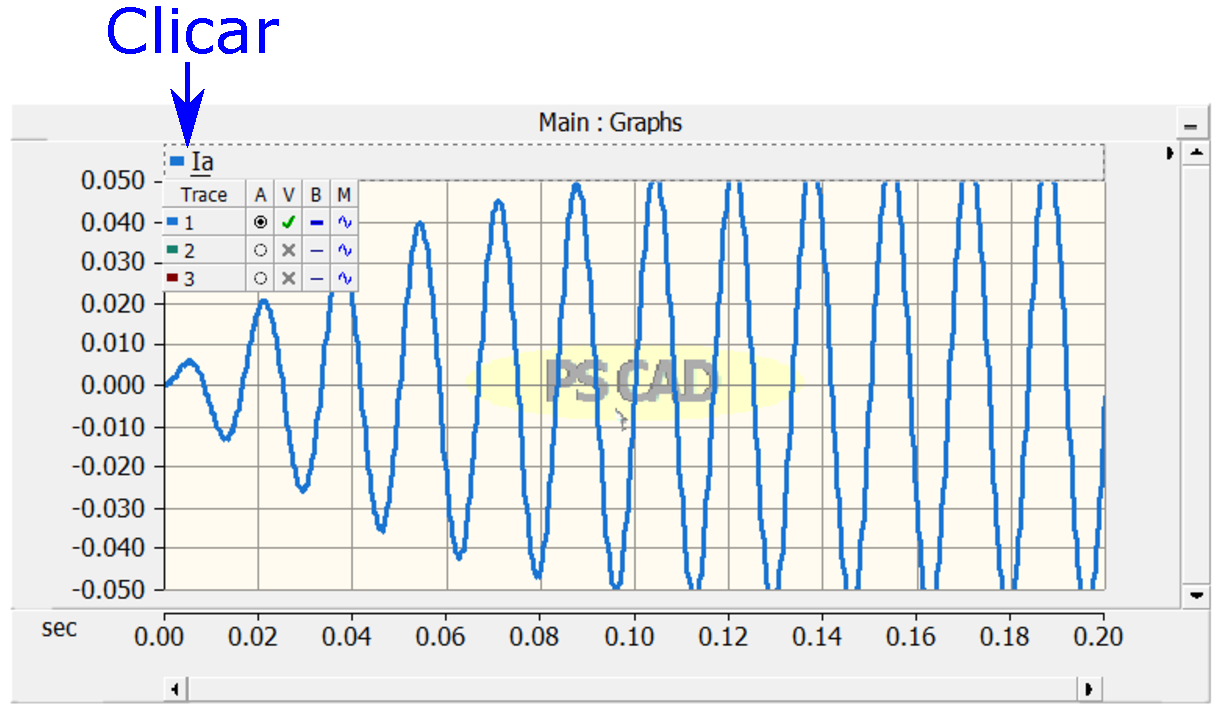
\includegraphics[width=0.9\linewidth]{./figuras/Visualizacao-resultados/graficos-Selecao}

\end{columns}

\end{frame}





%%%%%%%%%%%%%%%%%%%%%%%%%%%%%%%%%%%%%%%%%%%%%%%%
%%%%%%%%%%%%%%%%%%%%%%%%%%%%%%%%%%%%%%%%%%%%%%%%
%%%%%%%%%%%%%%%%%%%%%%%%%%%%%%%%%%%%%%%%%%%%%%%%
%%%%%%%%%%%%%%%%%%%%%%%%%%%%%%%%%%%%%%%%%%%%%%%%
\begin{frame}{Ajustes nos Gráficos: Escala}
\centering

\begin{columns}
\column{0.3\linewidth}

\begin{itemize}
\item Propriedades do gráfico
\vspace*{1cm}
\item Permite ajustar a escala
\vspace*{1cm}
\item Permite alterar a grade
\end{itemize}


\column{0.7\linewidth}
\centering
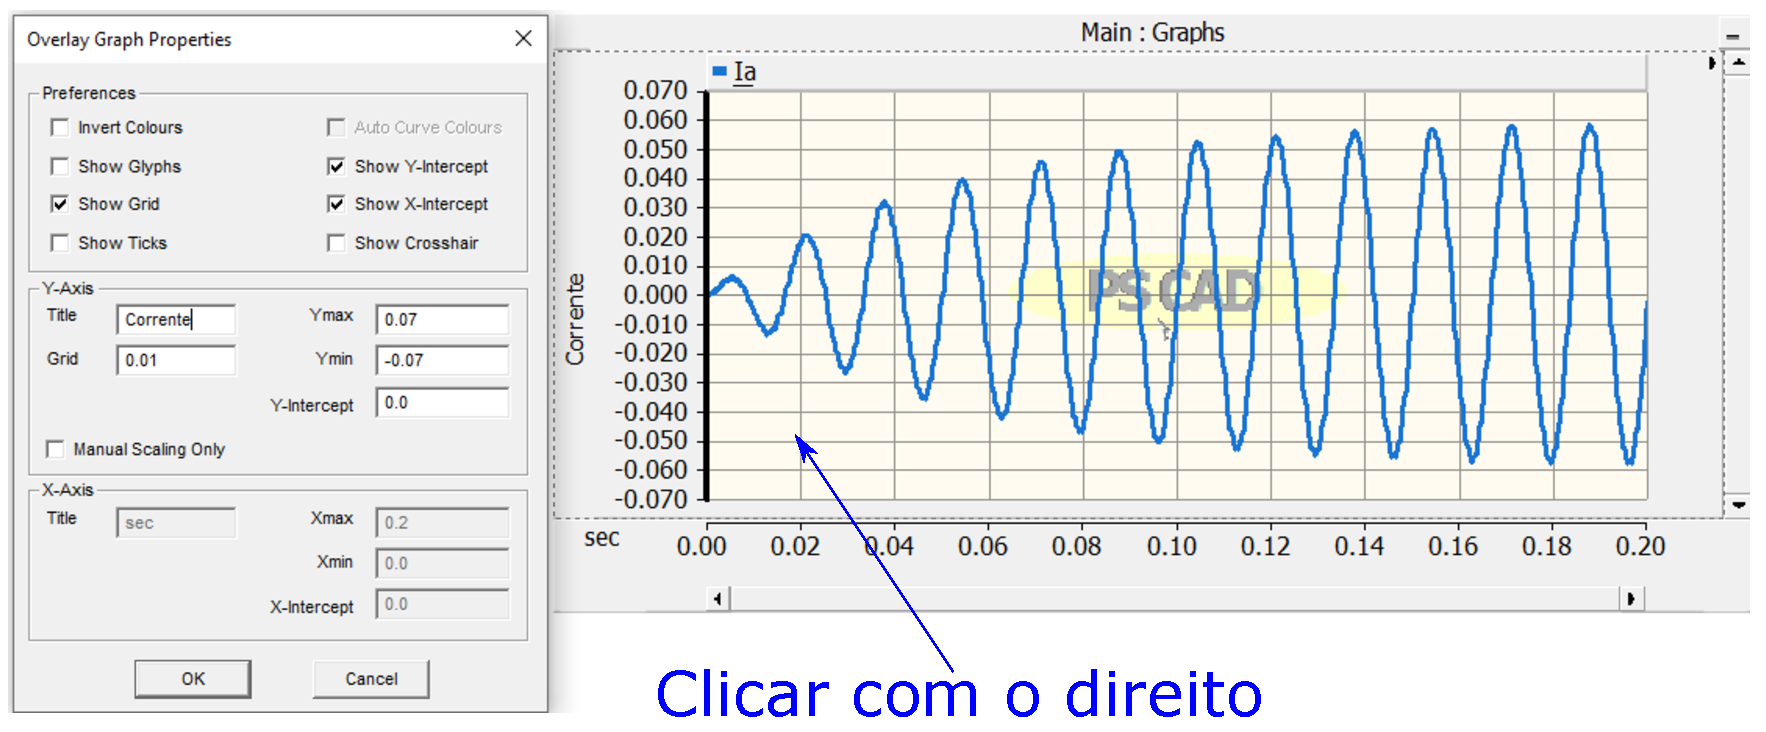
\includegraphics[width=0.9\linewidth]{./figuras/Visualizacao-resultados/graficos-escalas}

\end{columns}

\end{frame}





%%%%%%%%%%%%%%%%%%%%%%%%%%%%%%%%%%%%%%%%%%%%%%%%
%%%%%%%%%%%%%%%%%%%%%%%%%%%%%%%%%%%%%%%%%%%%%%%%
%%%%%%%%%%%%%%%%%%%%%%%%%%%%%%%%%%%%%%%%%%%%%%%%
%%%%%%%%%%%%%%%%%%%%%%%%%%%%%%%%%%%%%%%%%%%%%%%%
\begin{frame}{Ajustes nos Gráficos: Atalhos}

Depois de clicar no gráfico:
\vspace*{1cm}
\begin{itemize}
\item \textbf{E} - Ajusta a escala do tempo
\vspace*{0.75cm}
\item \textbf{Y} - Ajusta a escala y do gráfico para melhor visualização
\vspace*{0.75cm}
\item \textbf{B} - Ajusta a escala y do gráfico de acordo com a configuração do output chanel
\vspace*{0.75cm}
\item \textbf{M} - Habilita dois cursores 
\end{itemize}

\end{frame}




%%%%%%%%%%%%%%%%%%%%%%%%%%%%%%%%%%%%%%%%%%%%%%%%
%%%%%%%%%%%%%%%%%%%%%%%%%%%%%%%%%%%%%%%%%%%%%%%%
%%%%%%%%%%%%%%%%%%%%%%%%%%%%%%%%%%%%%%%%%%%%%%%%
%%%%%%%%%%%%%%%%%%%%%%%%%%%%%%%%%%%%%%%%%%%%%%%%
\begin{frame}{Ajustes nos Gráficos: Polygrphs}
\centering

\begin{columns}
\column{0.3\linewidth}

\begin{itemize}
\item Propriedades do gráfico
\vspace*{1cm}
\item Permite ajustar a escala
\vspace*{1cm}
\item Permite alterar a grade
\end{itemize}


\column{0.7\linewidth}
\centering
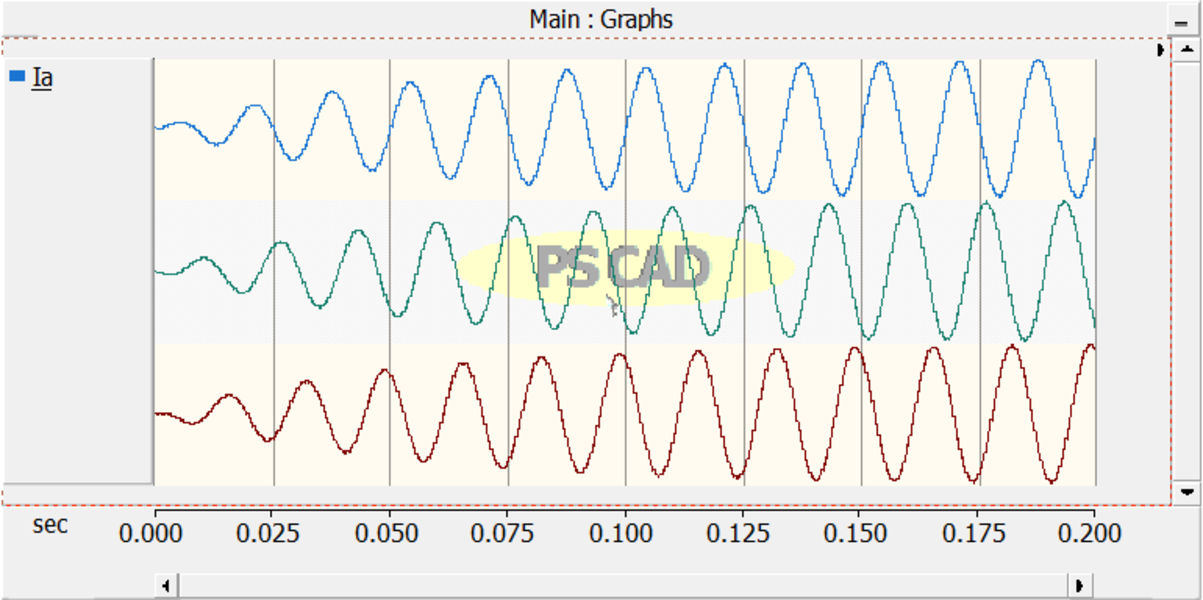
\includegraphics[width=0.9\linewidth]{./figuras/Visualizacao-resultados/graficos-polygraph}

\end{columns}

\end{frame}





%%%%%%%%%%%%%%%%%%%%%%%%%%%%%%%%%%%%%%%%%%%%%%%%
%%%%%%%%%%%%%%%%%%%%%%%%%%%%%%%%%%%%%%%%%%%%%%%%
%%%%%%%%%%%%%%%%%%%%%%%%%%%%%%%%%%%%%%%%%%%%%%%%
%%%%%%%%%%%%%%%%%%%%%%%%%%%%%%%%%%%%%%%%%%%%%%%%
\begin{frame}{Ajustes nos Gráficos: adicionando curvas ao gráfico}
\centering


\begin{columns}
\column{0.25\linewidth}

\begin{itemize}
\item Selecione o {\it output chanel}
\vspace*{1cm}
\item Precione a tecla {\it CTRL}
\vspace*{1cm}
\item Arraste em direção a um gráfico existente
\end{itemize}


\column{0.75\linewidth}
\centering
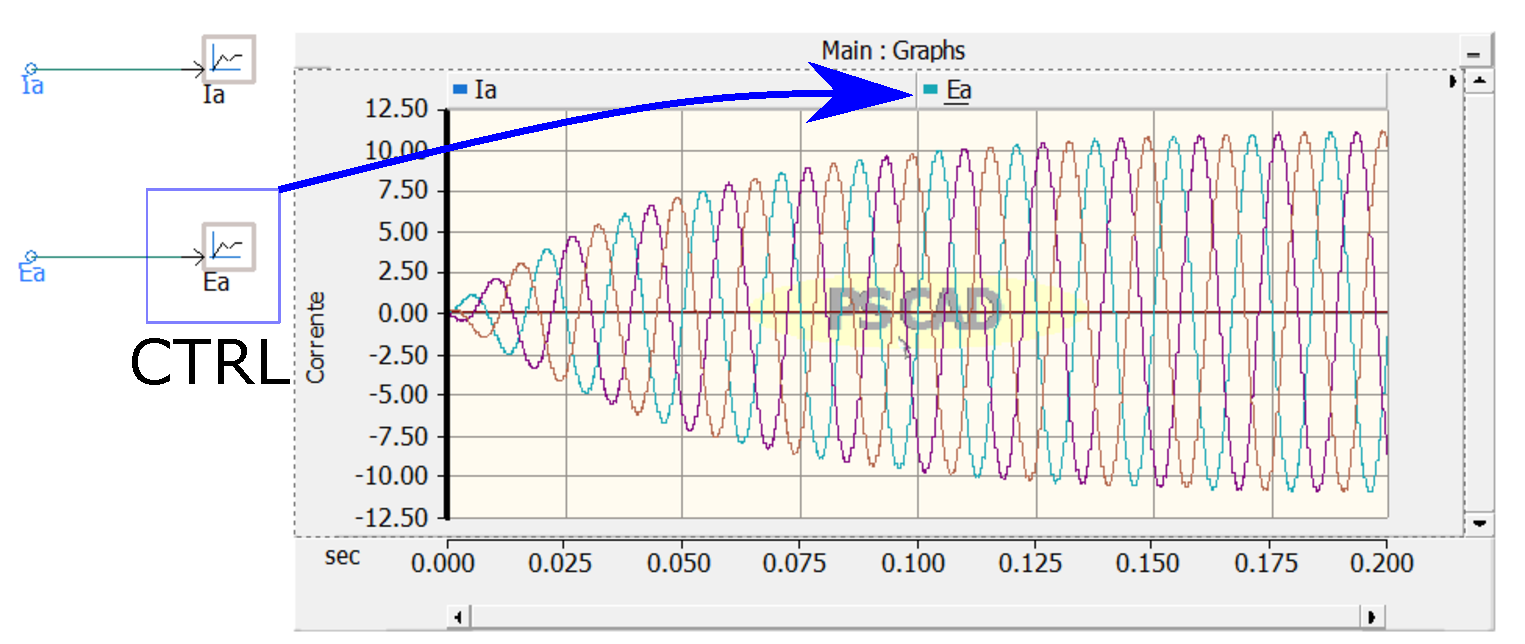
\includegraphics[width=0.95\linewidth]{./figuras/Visualizacao-resultados/graficos-add-curvas}

\end{columns}





\end{frame}






%%%%%%%%%%%%%%%%%%%%%%%%%%%%%%%%%%%%%%%%%%%%%%%%
%%%%%%%%%%%%%%%%%%%%%%%%%%%%%%%%%%%%%%%%%%%%%%%%
%%%%%%%%%%%%%%%%%%%%%%%%%%%%%%%%%%%%%%%%%%%%%%%%
%%%%%%%%%%%%%%%%%%%%%%%%%%%%%%%%%%%%%%%%%%%%%%%%
\begin{frame}{Ajustes nos Gráficos: Painéis de Controle}
\centering



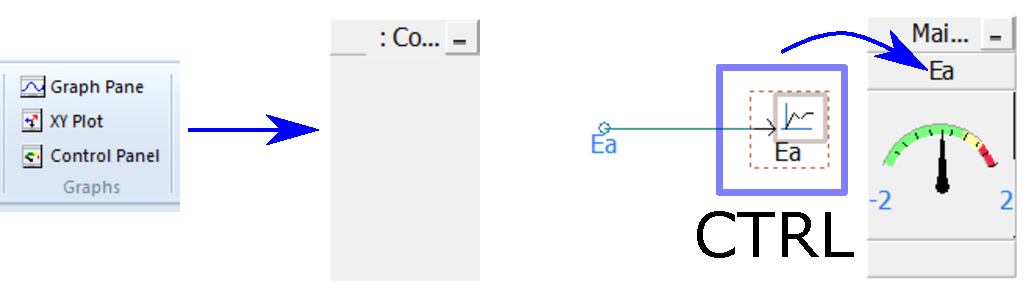
\includegraphics[width=0.95\linewidth]{./figuras/Visualizacao-resultados/graficos-Control-panel}




\end{frame}








%
%
%
%%%%%%%%%%%%%%%%%%%%%%%%%%%%%%%%%%%%%%%%%%%%%%%%%
%%%%%%%%%%%%%%%%%%%%%%%%%%%%%%%%%%%%%%%%%%%%%%%%%
%%%%%%%%%%%%%%%%%%%%%%%%%%%%%%%%%%%%%%%%%%%%%%%%%
%%%%%%%%%%%%%%%%%%%%%%%%%%%%%%%%%%%%%%%%%%%%%%%%%
%\begin{frame}{Ajustes nos Gráficos: Medidor Fasorial}
%\centering
%
%
%\end{frame}




\cmfnewsection{Circuitos Simples para Aprender Usar Outros Blocos}{./logos/fundo_tese}{0.15}








%%%%%%%%%%%%%%%%%%%%%%%%%%%%%%%%%%%%%%%%%%%%%%%%
%%%%%%%%%%%%%%%%%%%%%%%%%%%%%%%%%%%%%%%%%%%%%%%%
%%%%%%%%%%%%%%%%%%%%%%%%%%%%%%%%%%%%%%%%%%%%%%%%
%%%%%%%%%%%%%%%%%%%%%%%%%%%%%%%%%%%%%%%%%%%%%%%%
\begin{frame}{Circuito 2A}
\centering



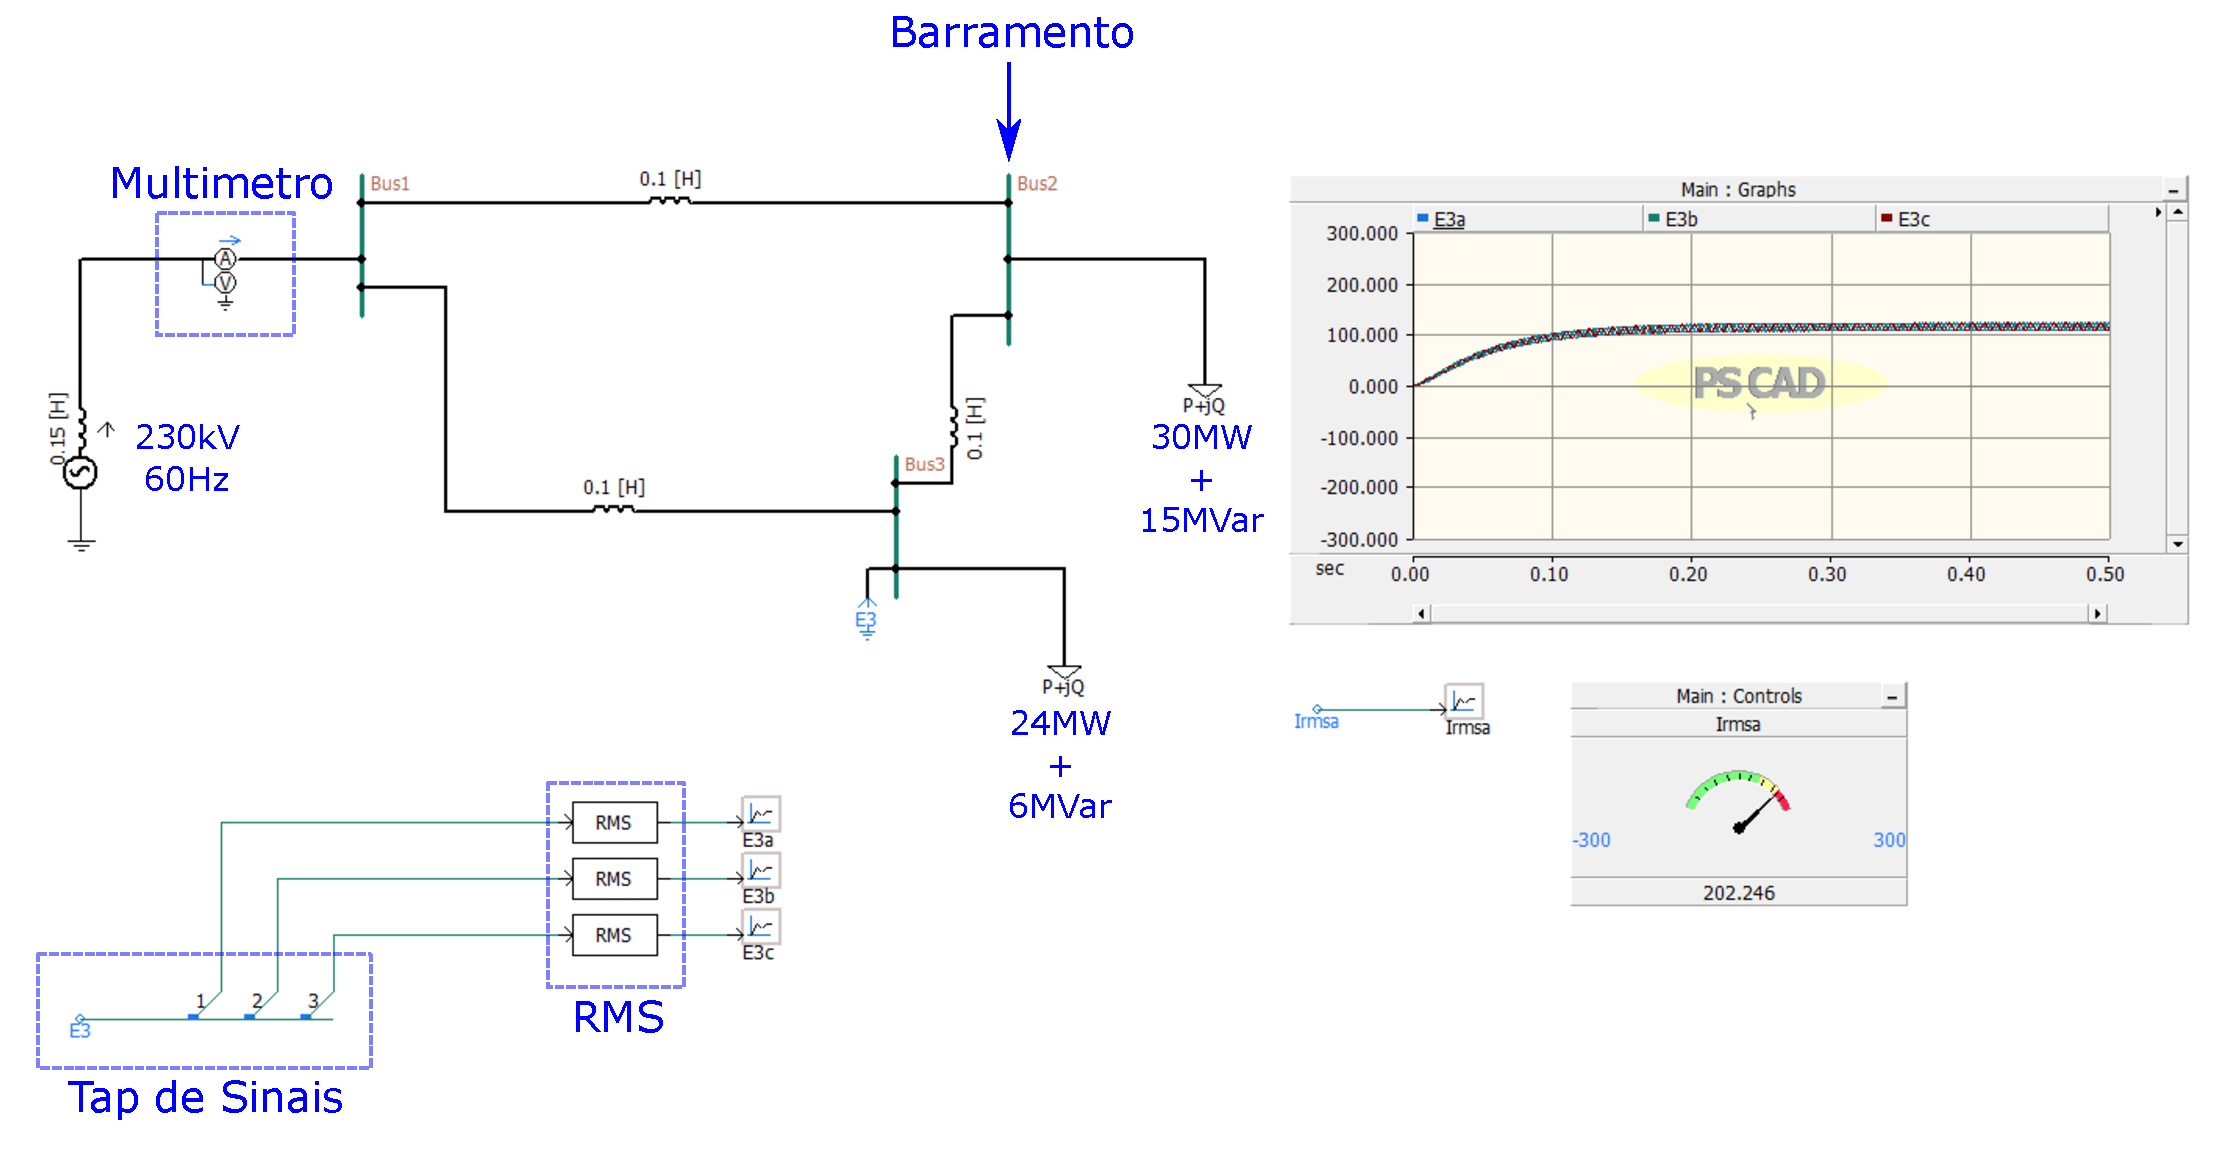
\includegraphics[width=0.95\linewidth]{./figuras/Segundo-Circuito/SIM2a}



\end{frame}






%%%%%%%%%%%%%%%%%%%%%%%%%%%%%%%%%%%%%%%%%%%%%%%%
%%%%%%%%%%%%%%%%%%%%%%%%%%%%%%%%%%%%%%%%%%%%%%%%
%%%%%%%%%%%%%%%%%%%%%%%%%%%%%%%%%%%%%%%%%%%%%%%%
%%%%%%%%%%%%%%%%%%%%%%%%%%%%%%%%%%%%%%%%%%%%%%%%
\begin{frame}{Circuito 2B}
\centering



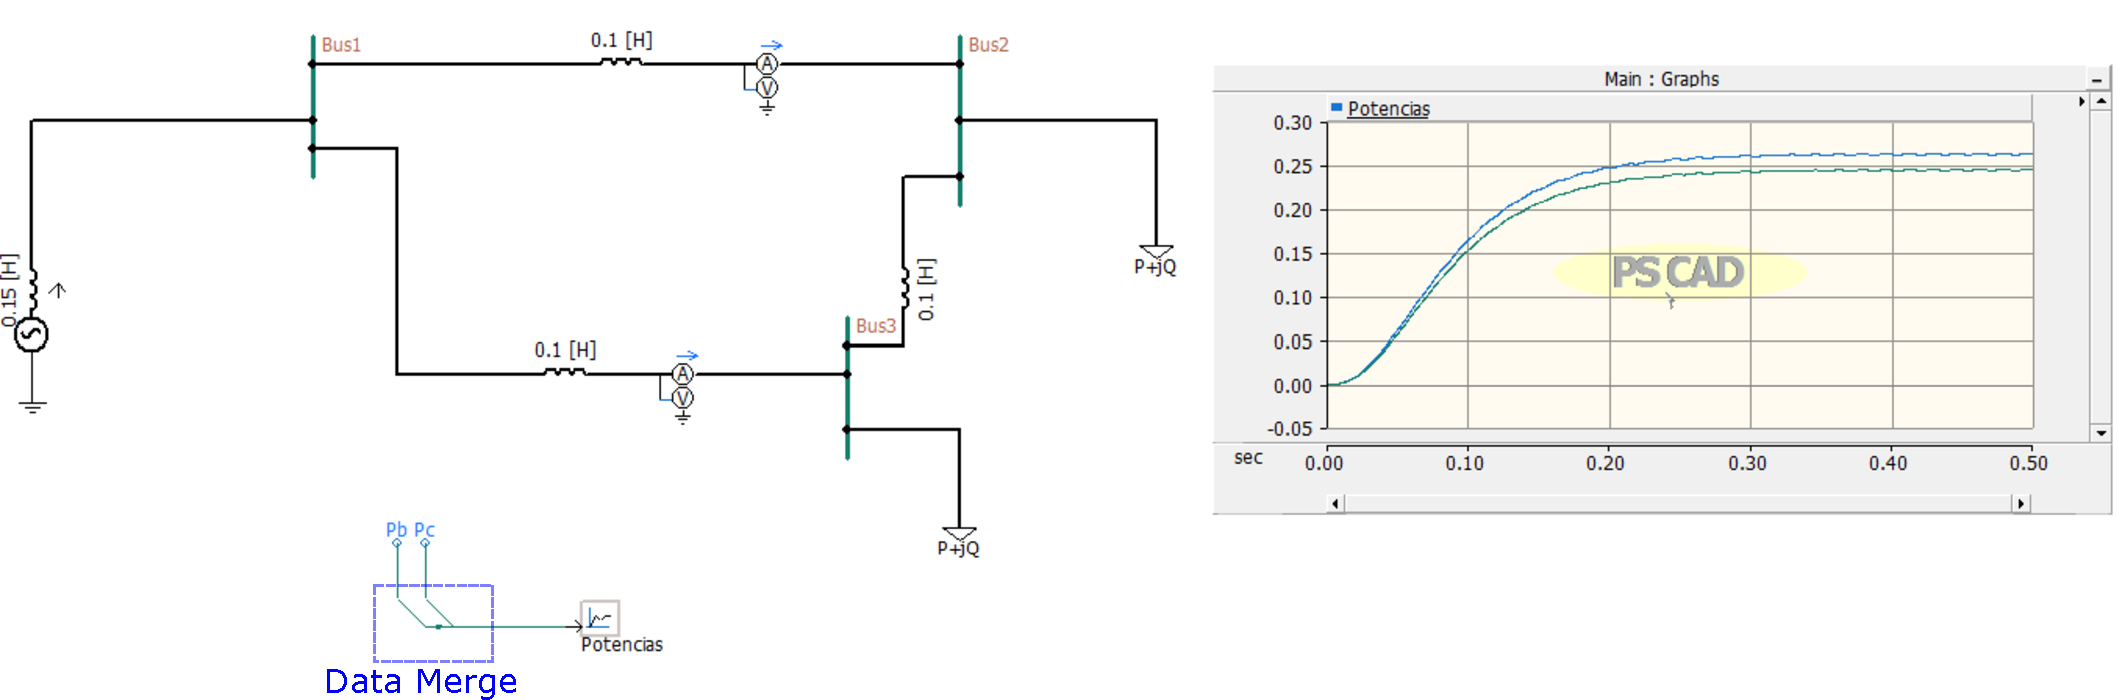
\includegraphics[width=0.95\linewidth]{./figuras/Segundo-Circuito/SIM2b}



\end{frame}







%%%%%%%%%%%%%%%%%%%%%%%%%%%%%%%%%%%%%%%%%%%%%%%%
%%%%%%%%%%%%%%%%%%%%%%%%%%%%%%%%%%%%%%%%%%%%%%%%
%%%%%%%%%%%%%%%%%%%%%%%%%%%%%%%%%%%%%%%%%%%%%%%%
%%%%%%%%%%%%%%%%%%%%%%%%%%%%%%%%%%%%%%%%%%%%%%%%
\begin{frame}{Circuito 2C}
\centering



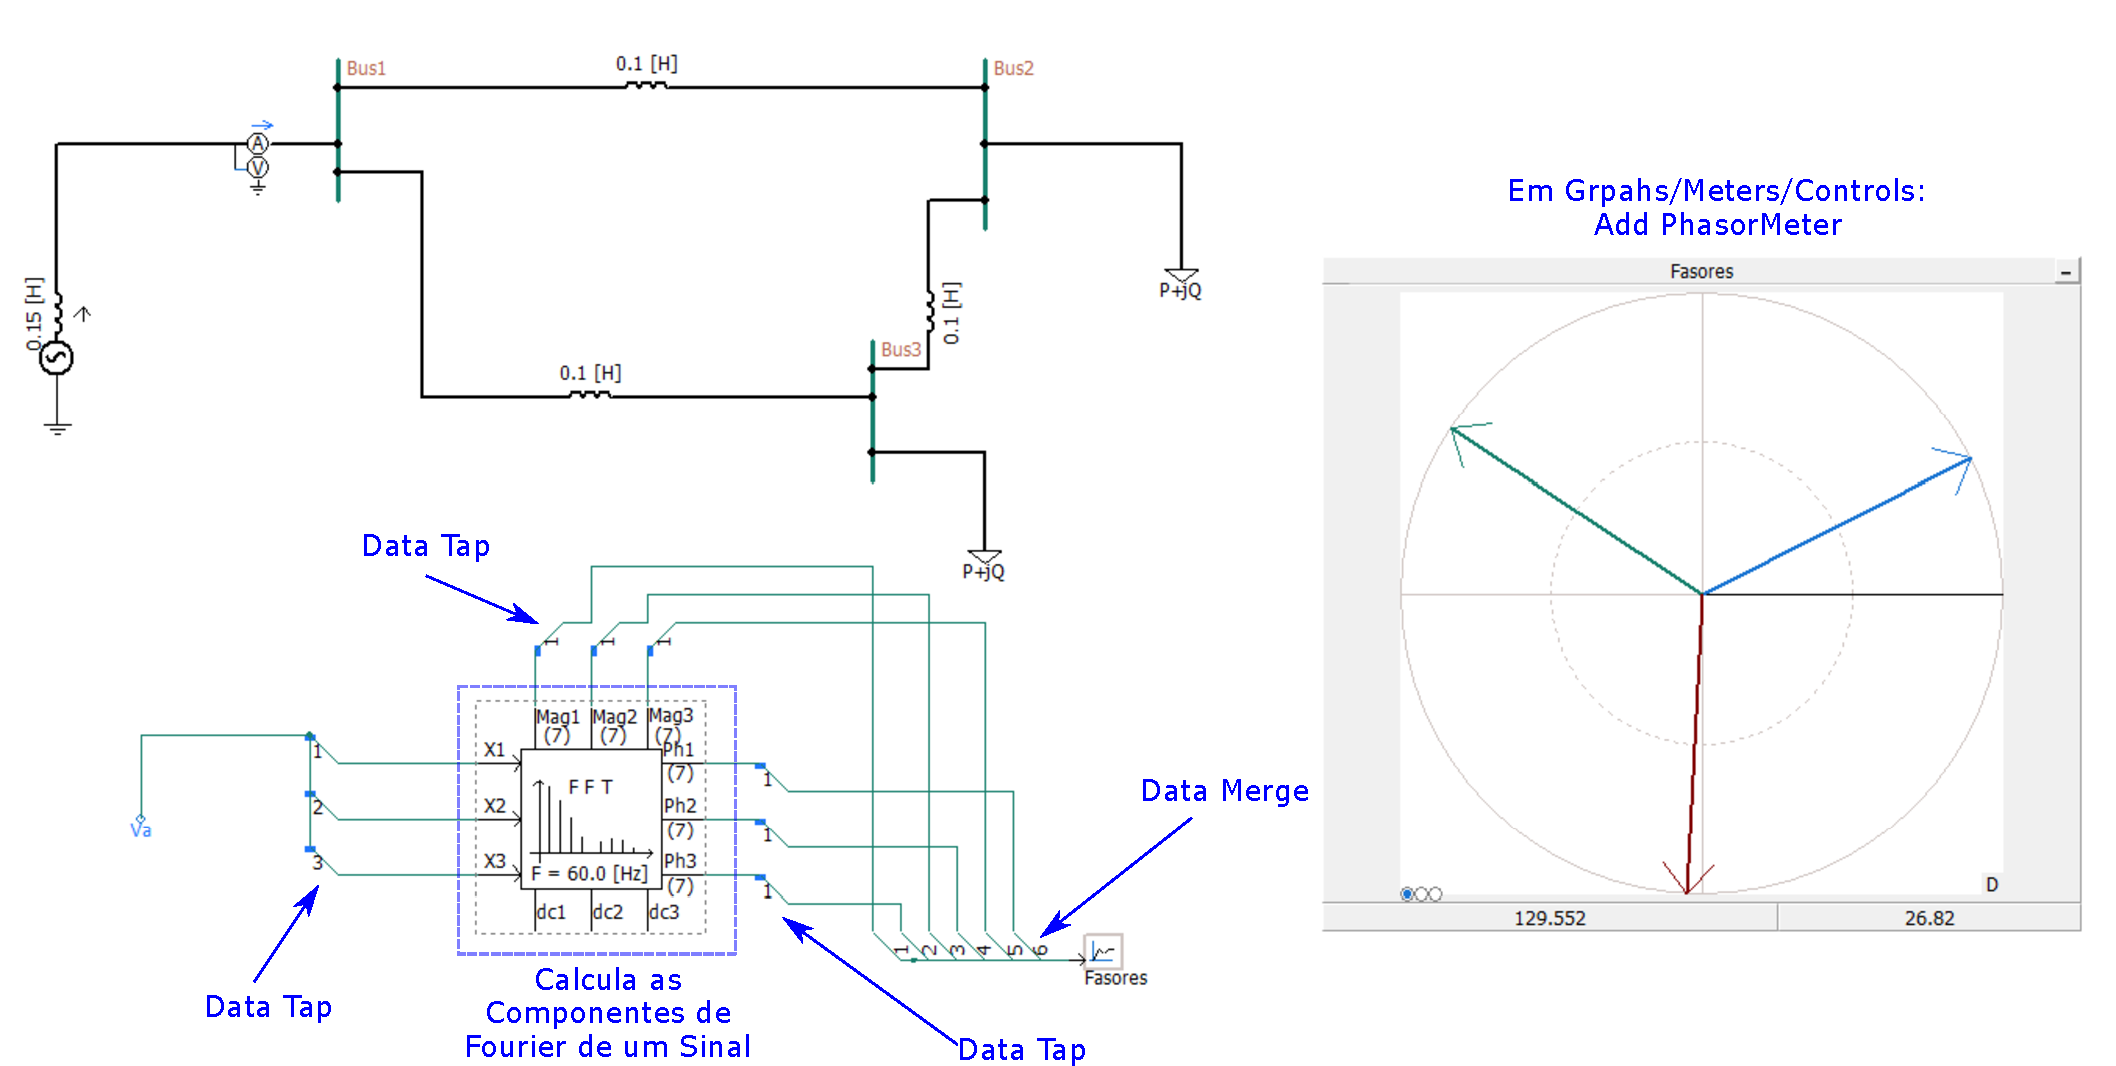
\includegraphics[width=0.95\linewidth]{./figuras/Segundo-Circuito/SIM2c}



\end{frame}







%%%%%%%%%%%%%%%%%%%%%%%%%%%%%%%%%%%%%%%%%%%%%%%%
%%%%%%%%%%%%%%%%%%%%%%%%%%%%%%%%%%%%%%%%%%%%%%%%
%%%%%%%%%%%%%%%%%%%%%%%%%%%%%%%%%%%%%%%%%%%%%%%%
%%%%%%%%%%%%%%%%%%%%%%%%%%%%%%%%%%%%%%%%%%%%%%%%
\begin{frame}{Circuito 2D: Nosso primeiro circuito monofásico}
\centering



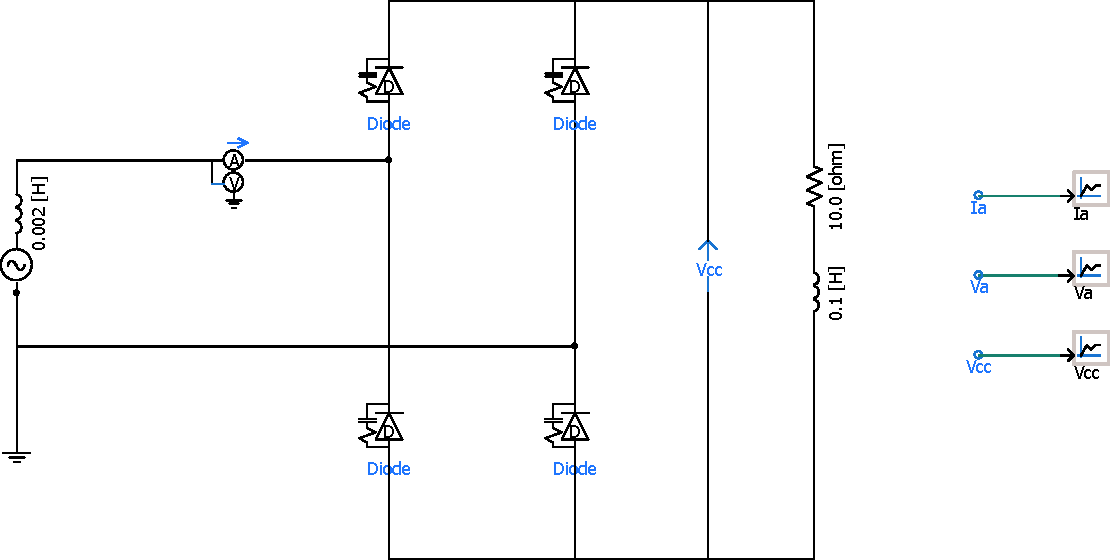
\includegraphics[width=0.75\linewidth]{./figuras/Segundo-Circuito/SIM2d}



\end{frame}






%%%%%%%%%%%%%%%%%%%%%%%%%%%%%%%%%%%%%%%%%%%%%%%%
%%%%%%%%%%%%%%%%%%%%%%%%%%%%%%%%%%%%%%%%%%%%%%%%
%%%%%%%%%%%%%%%%%%%%%%%%%%%%%%%%%%%%%%%%%%%%%%%%
%%%%%%%%%%%%%%%%%%%%%%%%%%%%%%%%%%%%%%%%%%%%%%%%
\begin{frame}{Circuito 2D: FFT}
\centering


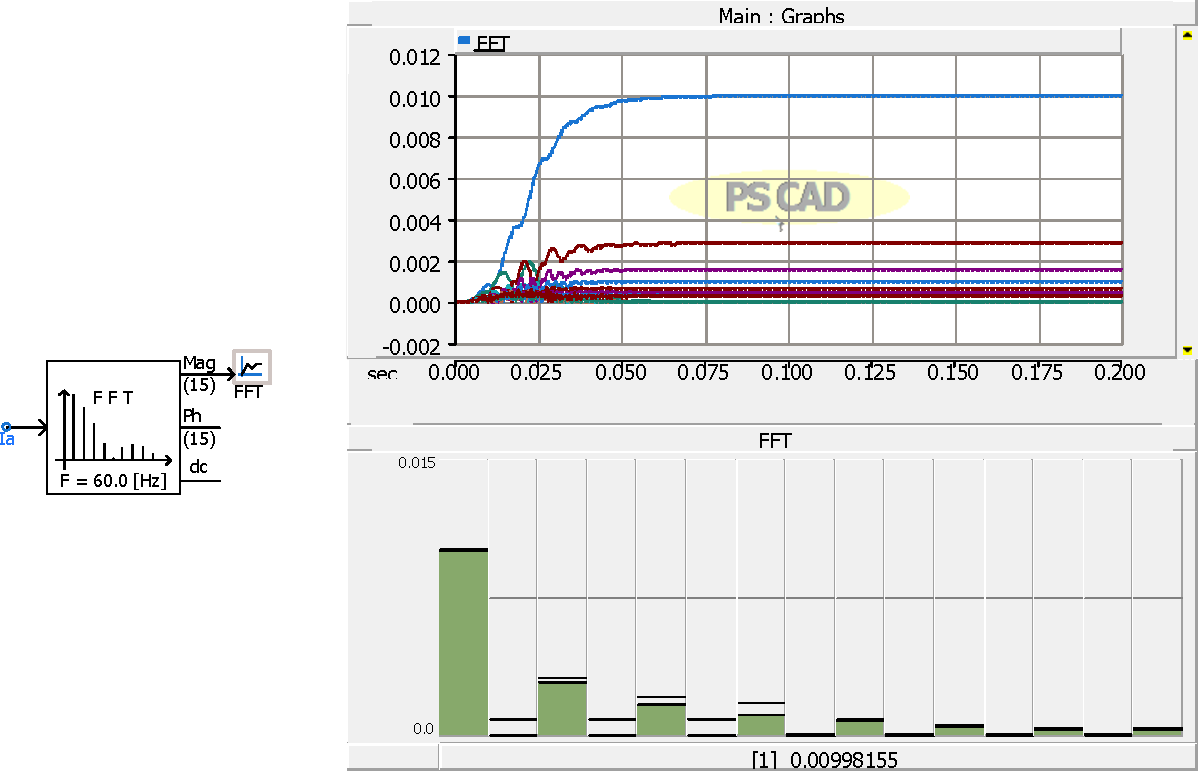
\includegraphics[width=0.70\linewidth]{./figuras/Segundo-Circuito/SIM2d-FFT}

\end{frame}




%%%%%%%%%%%%%%%%%%%%%%%%%%%%%%%%%%%%%%%%%%%%%%%%
%%%%%%%%%%%%%%%%%%%%%%%%%%%%%%%%%%%%%%%%%%%%%%%%
%%%%%%%%%%%%%%%%%%%%%%%%%%%%%%%%%%%%%%%%%%%%%%%%
%%%%%%%%%%%%%%%%%%%%%%%%%%%%%%%%%%%%%%%%%%%%%%%%
\begin{frame}{Circuito 2E: Transformadores e etc}
\centering


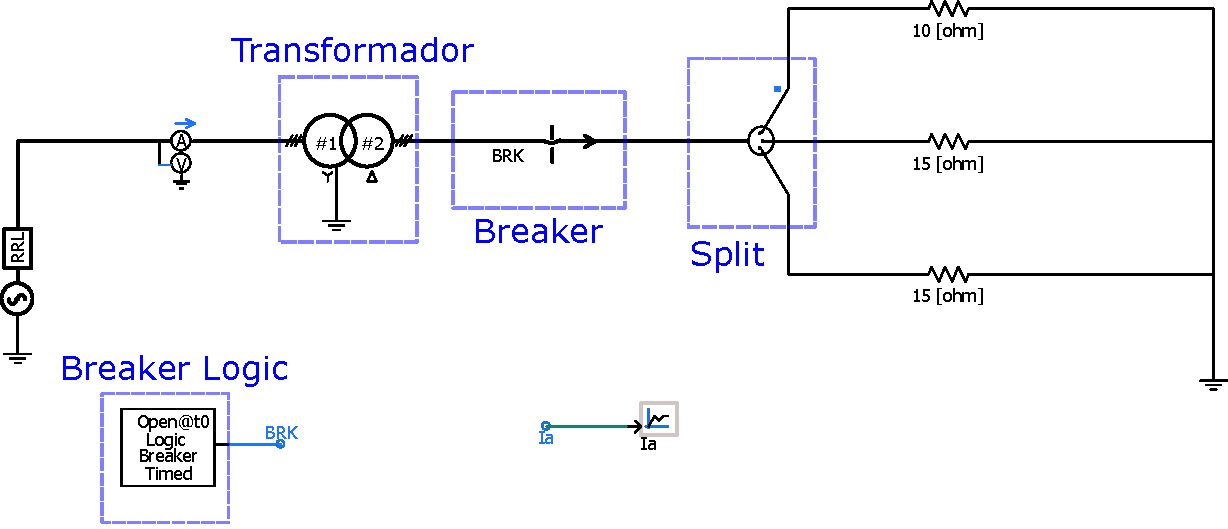
\includegraphics[width=0.70\linewidth]{./figuras/Segundo-Circuito/SIM2e}

\end{frame}






%%%%%%%%%%%%%%%%%%%%%%%%%%%%%%%%%%%%%%%%%%%%%%%%
%%%%%%%%%%%%%%%%%%%%%%%%%%%%%%%%%%%%%%%%%%%%%%%%
%%%%%%%%%%%%%%%%%%%%%%%%%%%%%%%%%%%%%%%%%%%%%%%%
%%%%%%%%%%%%%%%%%%%%%%%%%%%%%%%%%%%%%%%%%%%%%%%%
\begin{frame}{Circuito 2F: Máquinas CC}
\centering


\begin{columns}

\column{0.4\linewidth}
\centering
Máquina
\vspace*{0.5cm}

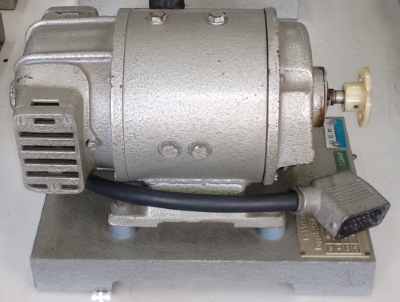
\includegraphics[width=0.95\linewidth]{./figuras/Segundo-Circuito/maquina_CC_b}

\column{0.6\linewidth}
\centering
Modelo Matemático\footnote[frame]{\tiny Stephen J. Chapman, Fundamentos das Máquinas Elétricas. 5ed. Capítulos 7 e 8.}
\vspace*{1cm}

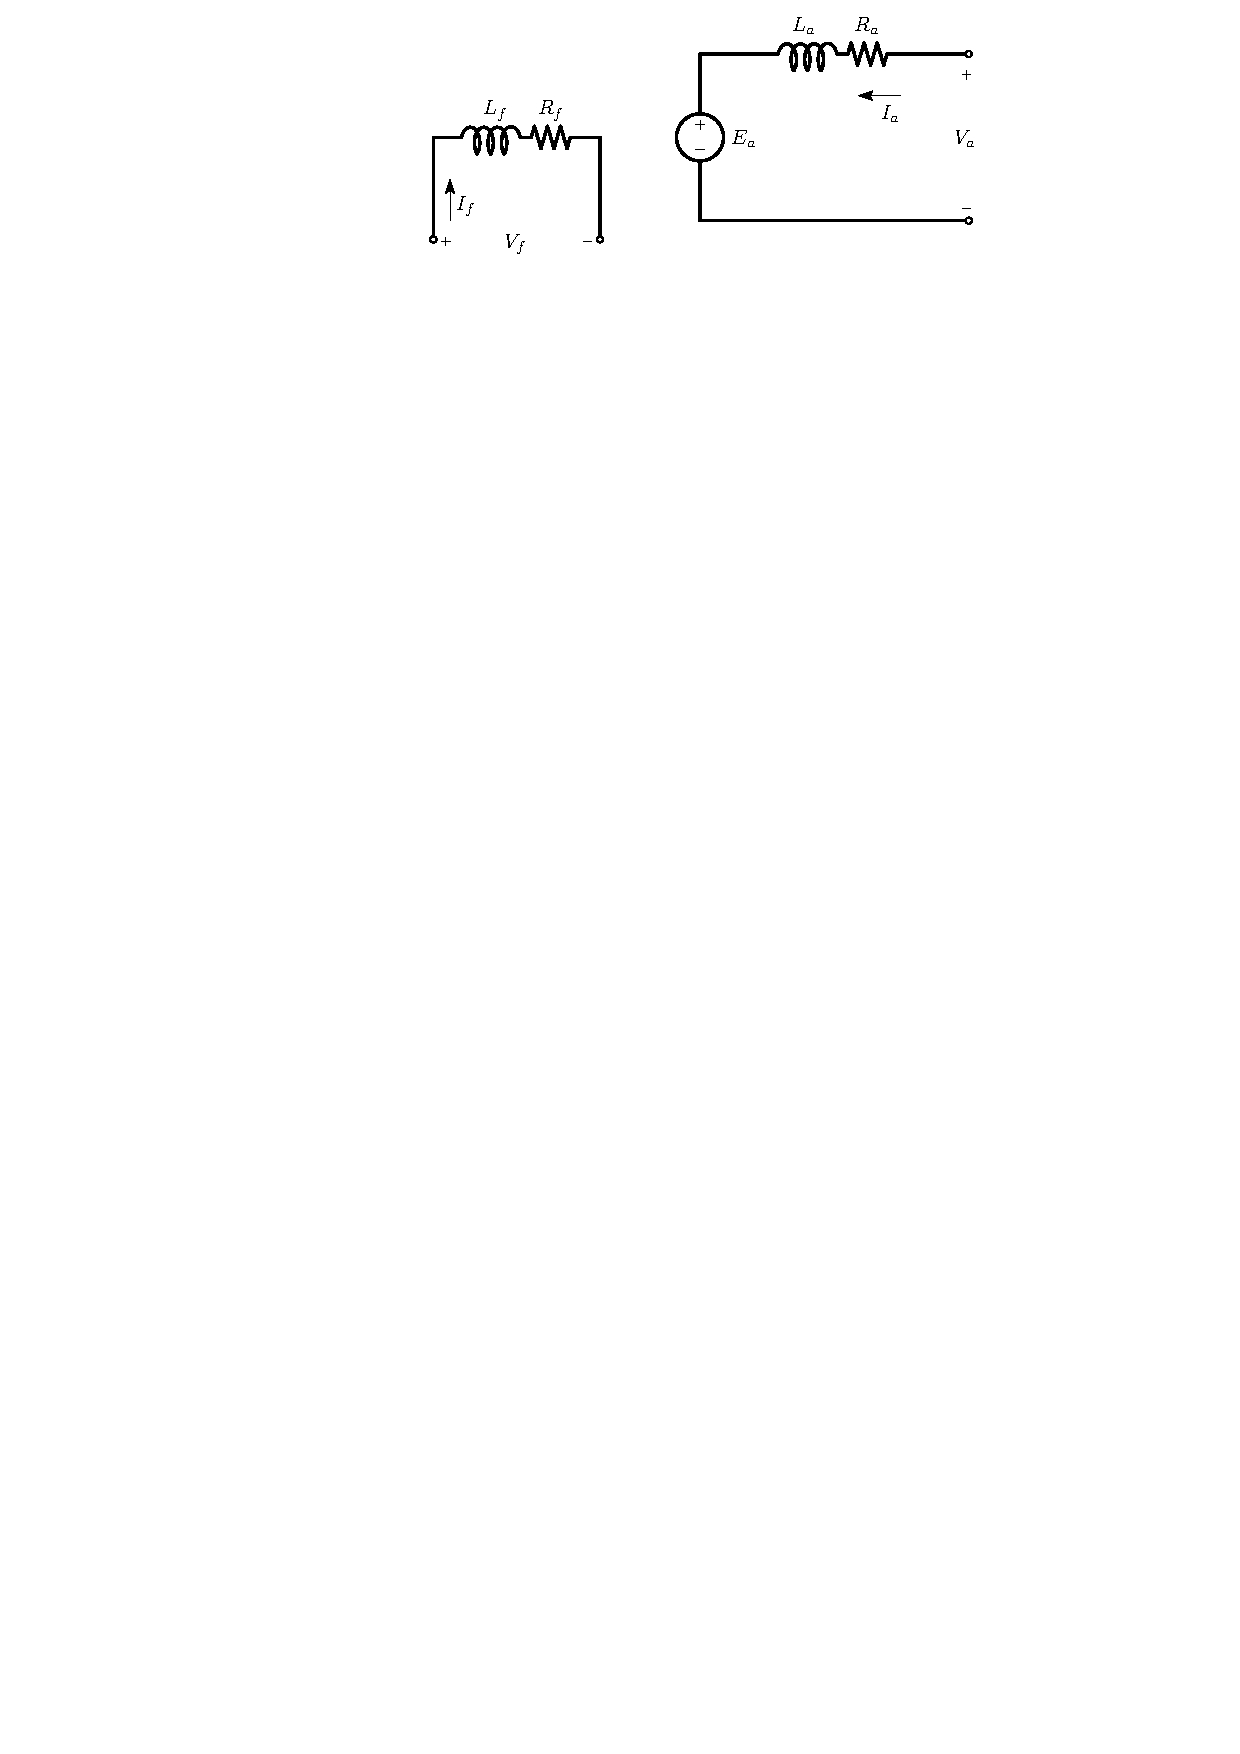
\includegraphics[width=0.95\linewidth]{./figuras/Segundo-Circuito/SIMf_dc_machine}

\end{columns}

\end{frame}





%%%%%%%%%%%%%%%%%%%%%%%%%%%%%%%%%%%%%%%%%%%%%%%%
%%%%%%%%%%%%%%%%%%%%%%%%%%%%%%%%%%%%%%%%%%%%%%%%
%%%%%%%%%%%%%%%%%%%%%%%%%%%%%%%%%%%%%%%%%%%%%%%%
%%%%%%%%%%%%%%%%%%%%%%%%%%%%%%%%%%%%%%%%%%%%%%%%
\begin{frame}{Circuito 2F: Mais Sobre o Modelo da Máquina}
\centering


\begin{columns}



\column{0.25\linewidth}
\centering

{\color{blue}Movimento

+

Fluxo  Magnético

$\downarrow$ 

Tensão Induzida
}





\column{0.5\linewidth}
\centering


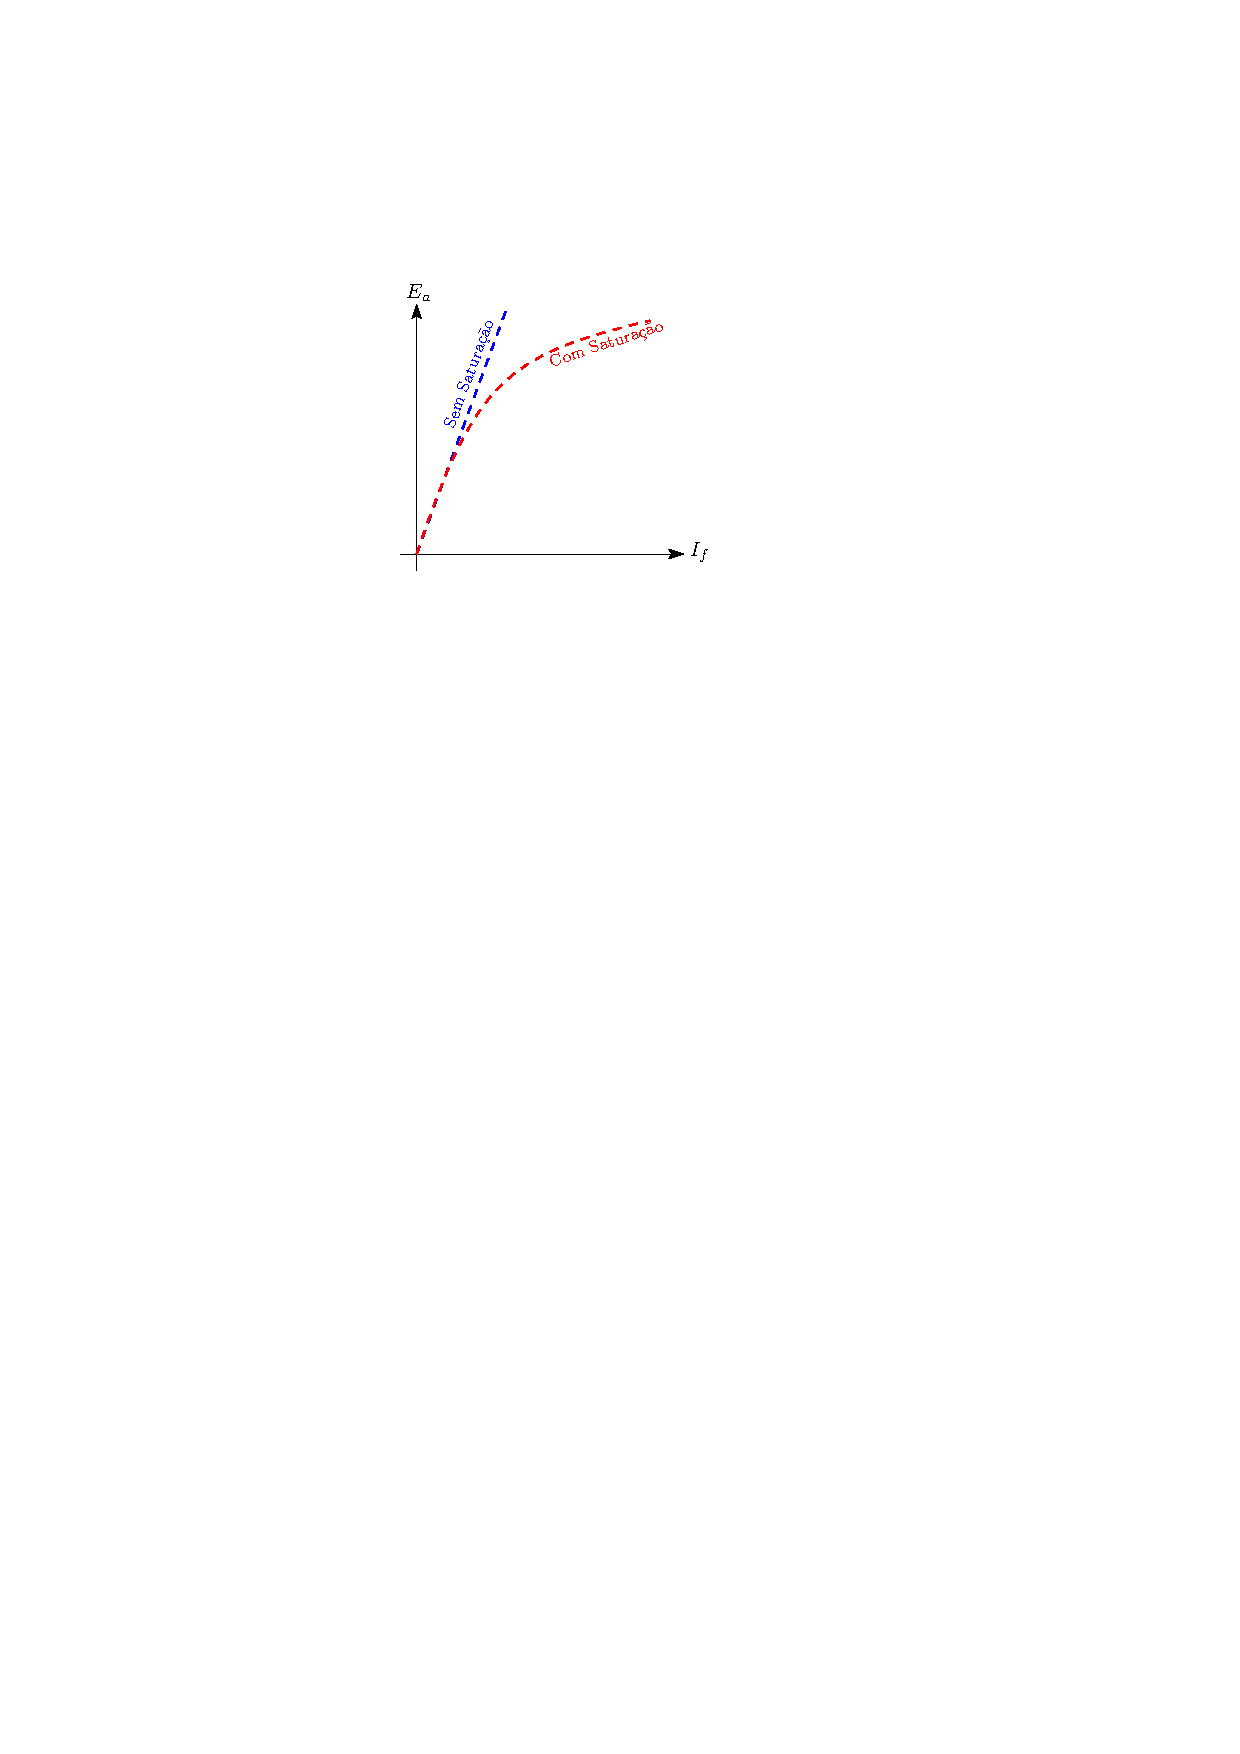
\includegraphics[width=0.85\linewidth]{./figuras/Segundo-Circuito/SIMf_dc_machine_excitation}




\column{0.25\linewidth}
\centering

{\color{blue}Corrente

+

Fluxo  Magnético

$\downarrow$ 

Torque
}

\end{columns}
\end{frame}




%%%%%%%%%%%%%%%%%%%%%%%%%%%%%%%%%%%%%%%%%%%%%%%%
%%%%%%%%%%%%%%%%%%%%%%%%%%%%%%%%%%%%%%%%%%%%%%%%
%%%%%%%%%%%%%%%%%%%%%%%%%%%%%%%%%%%%%%%%%%%%%%%%
%%%%%%%%%%%%%%%%%%%%%%%%%%%%%%%%%%%%%%%%%%%%%%%%
\begin{frame}{Circuito 2F: Máquinas CC no PSCAD}
\centering


\begin{columns}

\column{0.4\linewidth}
\centering

\begin{itemize}
\item Representa apenas as equações elétricas 
\vspace*{2cm}
\item A dinâmica mecânica é deixada de lado
\end{itemize}

\column{0.6\linewidth}
\centering


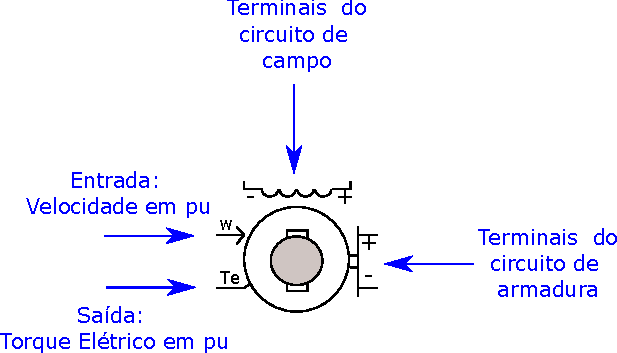
\includegraphics[width=0.95\linewidth]{./figuras/Segundo-Circuito/SEMf_maq_cc_pascad}

\end{columns}
\end{frame}




%%%%%%%%%%%%%%%%%%%%%%%%%%%%%%%%%%%%%%%%%%%%%%%%
%%%%%%%%%%%%%%%%%%%%%%%%%%%%%%%%%%%%%%%%%%%%%%%%
%%%%%%%%%%%%%%%%%%%%%%%%%%%%%%%%%%%%%%%%%%%%%%%%
%%%%%%%%%%%%%%%%%%%%%%%%%%%%%%%%%%%%%%%%%%%%%%%%
\begin{frame}{Circuito 2F: Modelando a Dinâmica Mecânica}
\centering


\begin{columns}

\column{0.5\linewidth}

{\it Lei de Newton} dos sistemas rotacionais:
\begin{equation*}
J \frac{d \omega_m}{dt} = T_e - T_m 
\end{equation*}



\column{0.5\linewidth}

Convertendo para pu: 
\begin{equation*}
2 H \frac{d \omega_{m,pu}}{dt}  = T_{e,pu} - T_{m,pu} 
\end{equation*}




\end{columns}

\begin{equation*}
H = \frac{J}{2}  \frac{\omega_{nominal}}{P_{nominal}}
\end{equation*}

\begin{itemize}
\item $T_e$ - Torque eletromagnético (calculado pelo modelo da máquina)
\item $T_m$ - Torque mecânico 
\item $\omega_m$ - Velocidade mecânica
\end{itemize}

\end{frame}







%%%%%%%%%%%%%%%%%%%%%%%%%%%%%%%%%%%%%%%%%%%%%%%%
%%%%%%%%%%%%%%%%%%%%%%%%%%%%%%%%%%%%%%%%%%%%%%%%
%%%%%%%%%%%%%%%%%%%%%%%%%%%%%%%%%%%%%%%%%%%%%%%%
%%%%%%%%%%%%%%%%%%%%%%%%%%%%%%%%%%%%%%%%%%%%%%%%
\begin{frame}{Circuito 2F: Circuito}
\centering

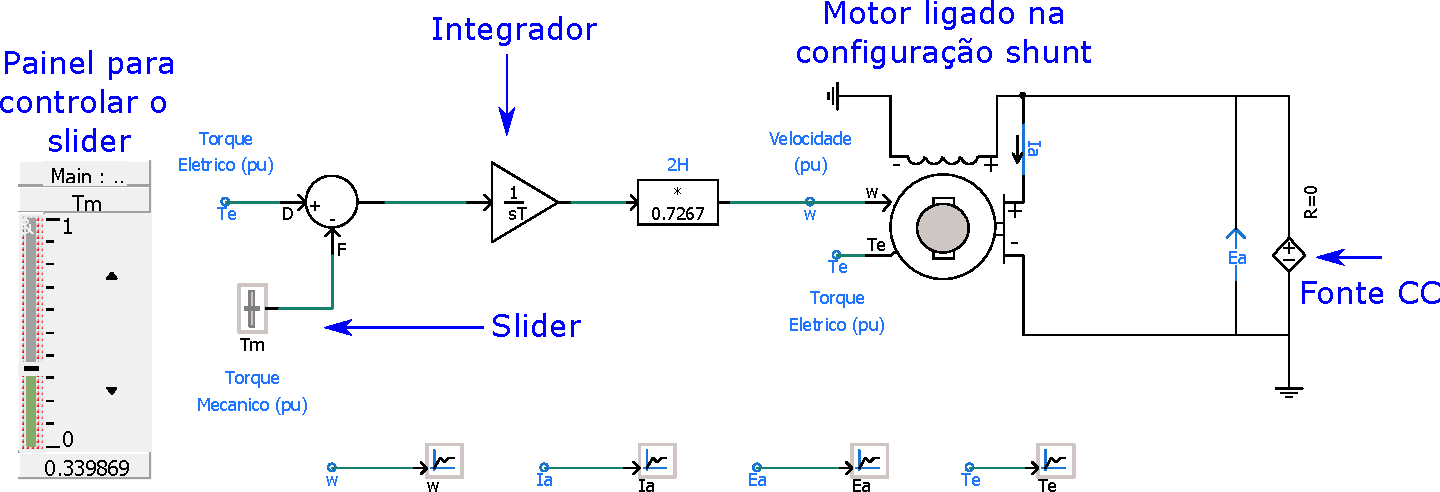
\includegraphics[width=0.9\linewidth]{./figuras/Segundo-Circuito/SIM2f}

\end{frame}
\cmfnewsection{Exportando Dados}{./logos/fundo_tese}{0.15}






%%%%%%%%%%%%%%%%%%%%%%%%%%%%%%%%%%%%%%%%%%%%%%%%
%%%%%%%%%%%%%%%%%%%%%%%%%%%%%%%%%%%%%%%%%%%%%%%%
%%%%%%%%%%%%%%%%%%%%%%%%%%%%%%%%%%%%%%%%%%%%%%%%
%%%%%%%%%%%%%%%%%%%%%%%%%%%%%%%%%%%%%%%%%%%%%%%%
\begin{frame}{Porque Exportar Dados?}
\centering


\textbf{Motivo 1:} Para produzir gráficos com melhor qualidade 
\vspace*{1cm}

\begin{columns}

\column{0.5\linewidth}
\centering
\textbf{PSCAD}
\vspace*{0.5cm}

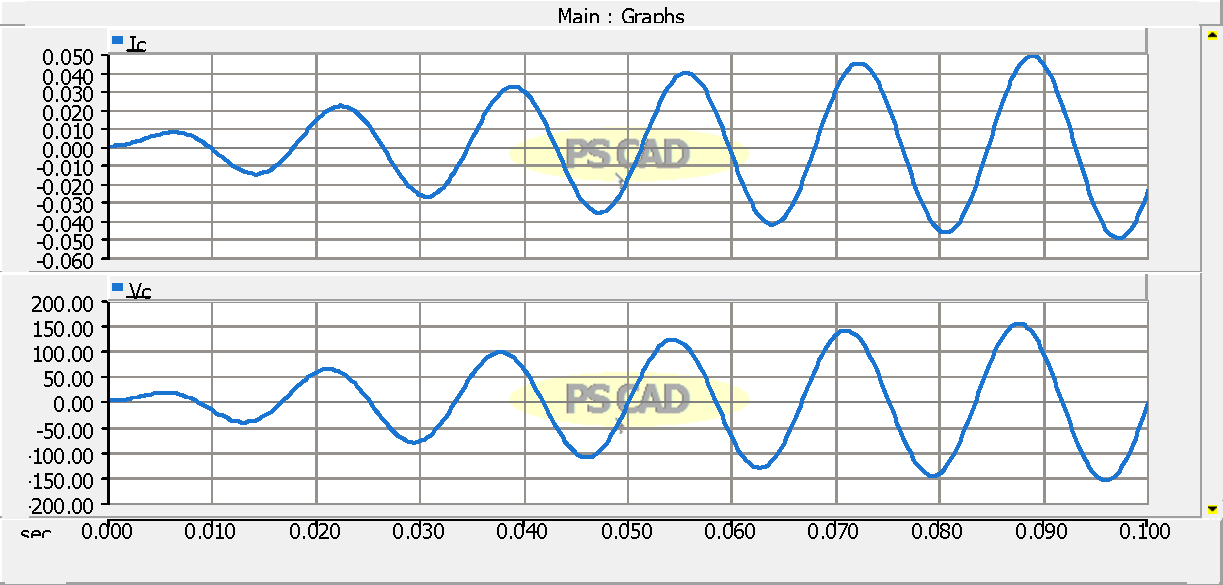
\includegraphics[width=0.90\linewidth]{./figuras/Exportacao/ex_pscadfig}
\column{0.5\linewidth}
\centering
\textbf{MATLAB/OCTAVE/matplotlib/etc}
\vspace*{0.5cm}

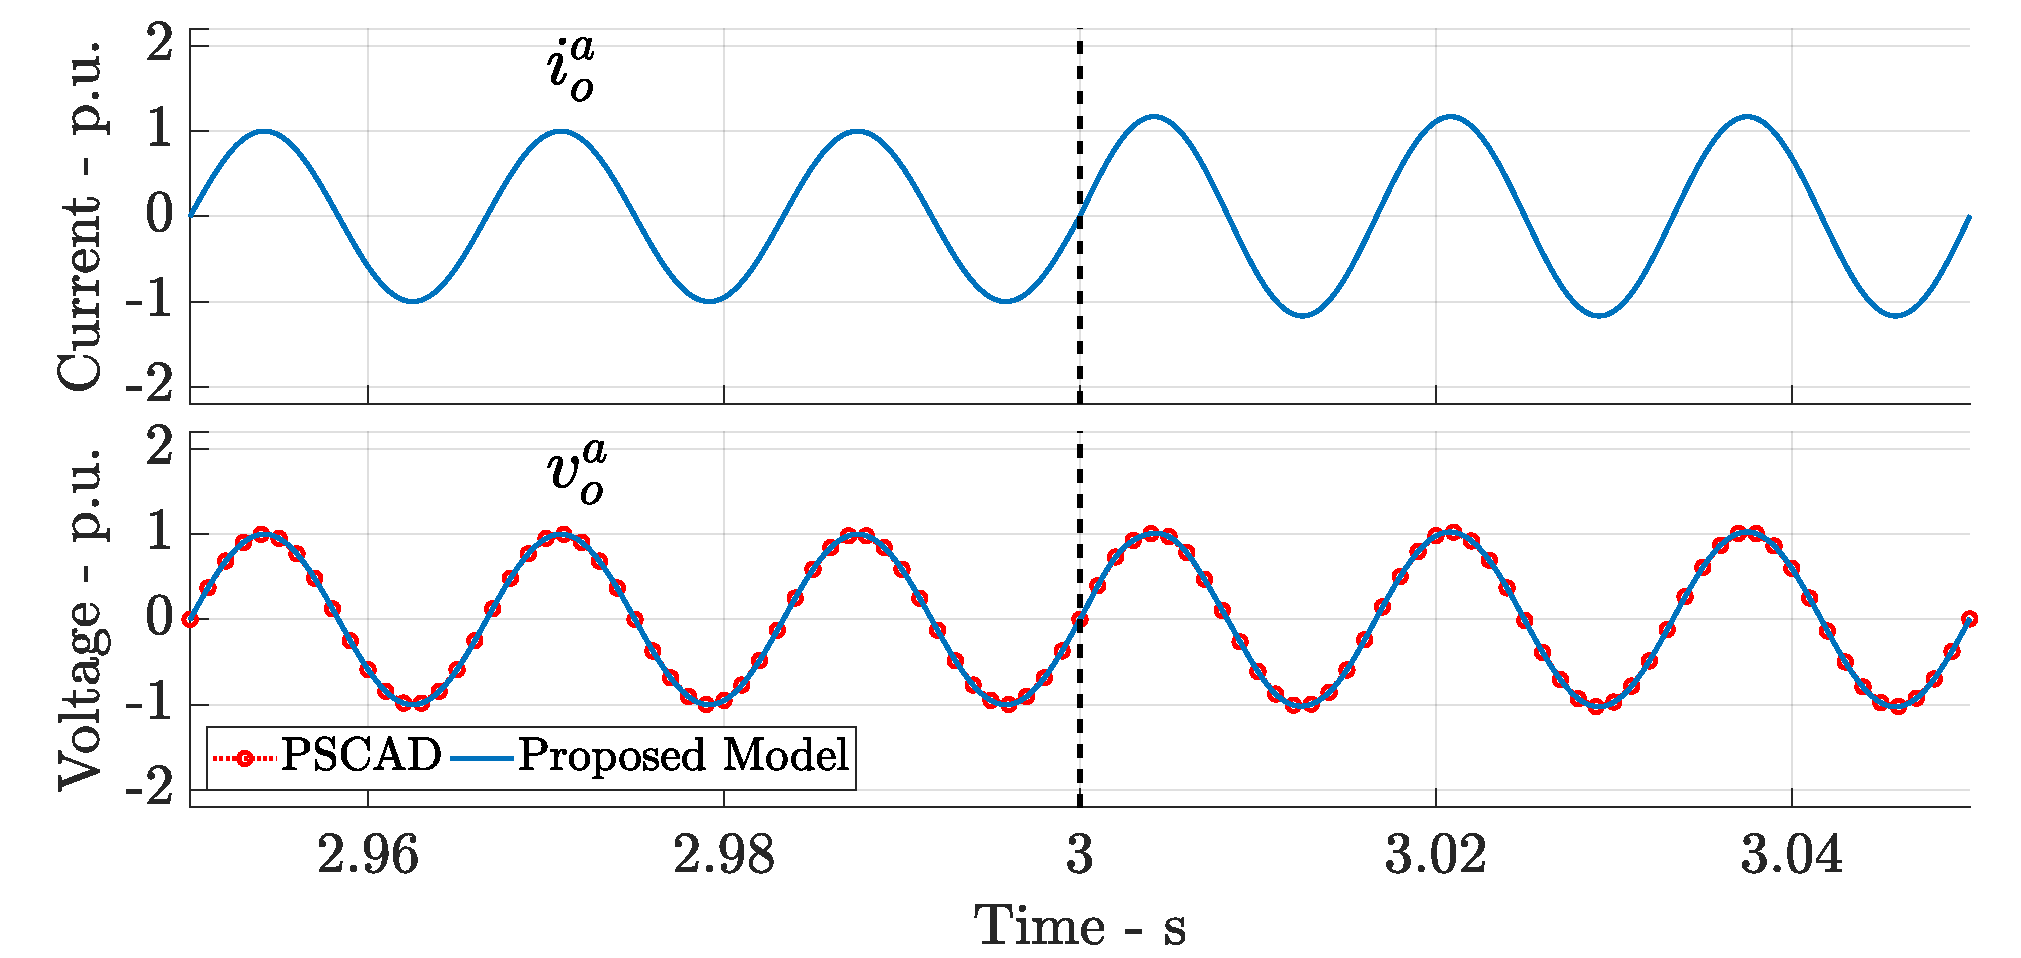
\includegraphics[width=0.90\linewidth]{./figuras/Exportacao/ex_matlab}

\end{columns}

\end{frame}





%%%%%%%%%%%%%%%%%%%%%%%%%%%%%%%%%%%%%%%%%%%%%%%%
%%%%%%%%%%%%%%%%%%%%%%%%%%%%%%%%%%%%%%%%%%%%%%%%
%%%%%%%%%%%%%%%%%%%%%%%%%%%%%%%%%%%%%%%%%%%%%%%%
%%%%%%%%%%%%%%%%%%%%%%%%%%%%%%%%%%%%%%%%%%%%%%%%
\begin{frame}{Porque Exportar Dados?}
\centering


\textbf{Motivo 2:} Para produzir gráficos de variáveis/funções indiretamente obtidas
\vspace*{1cm}

\textbf{Diagrama de bode}
\vspace*{0.5cm}

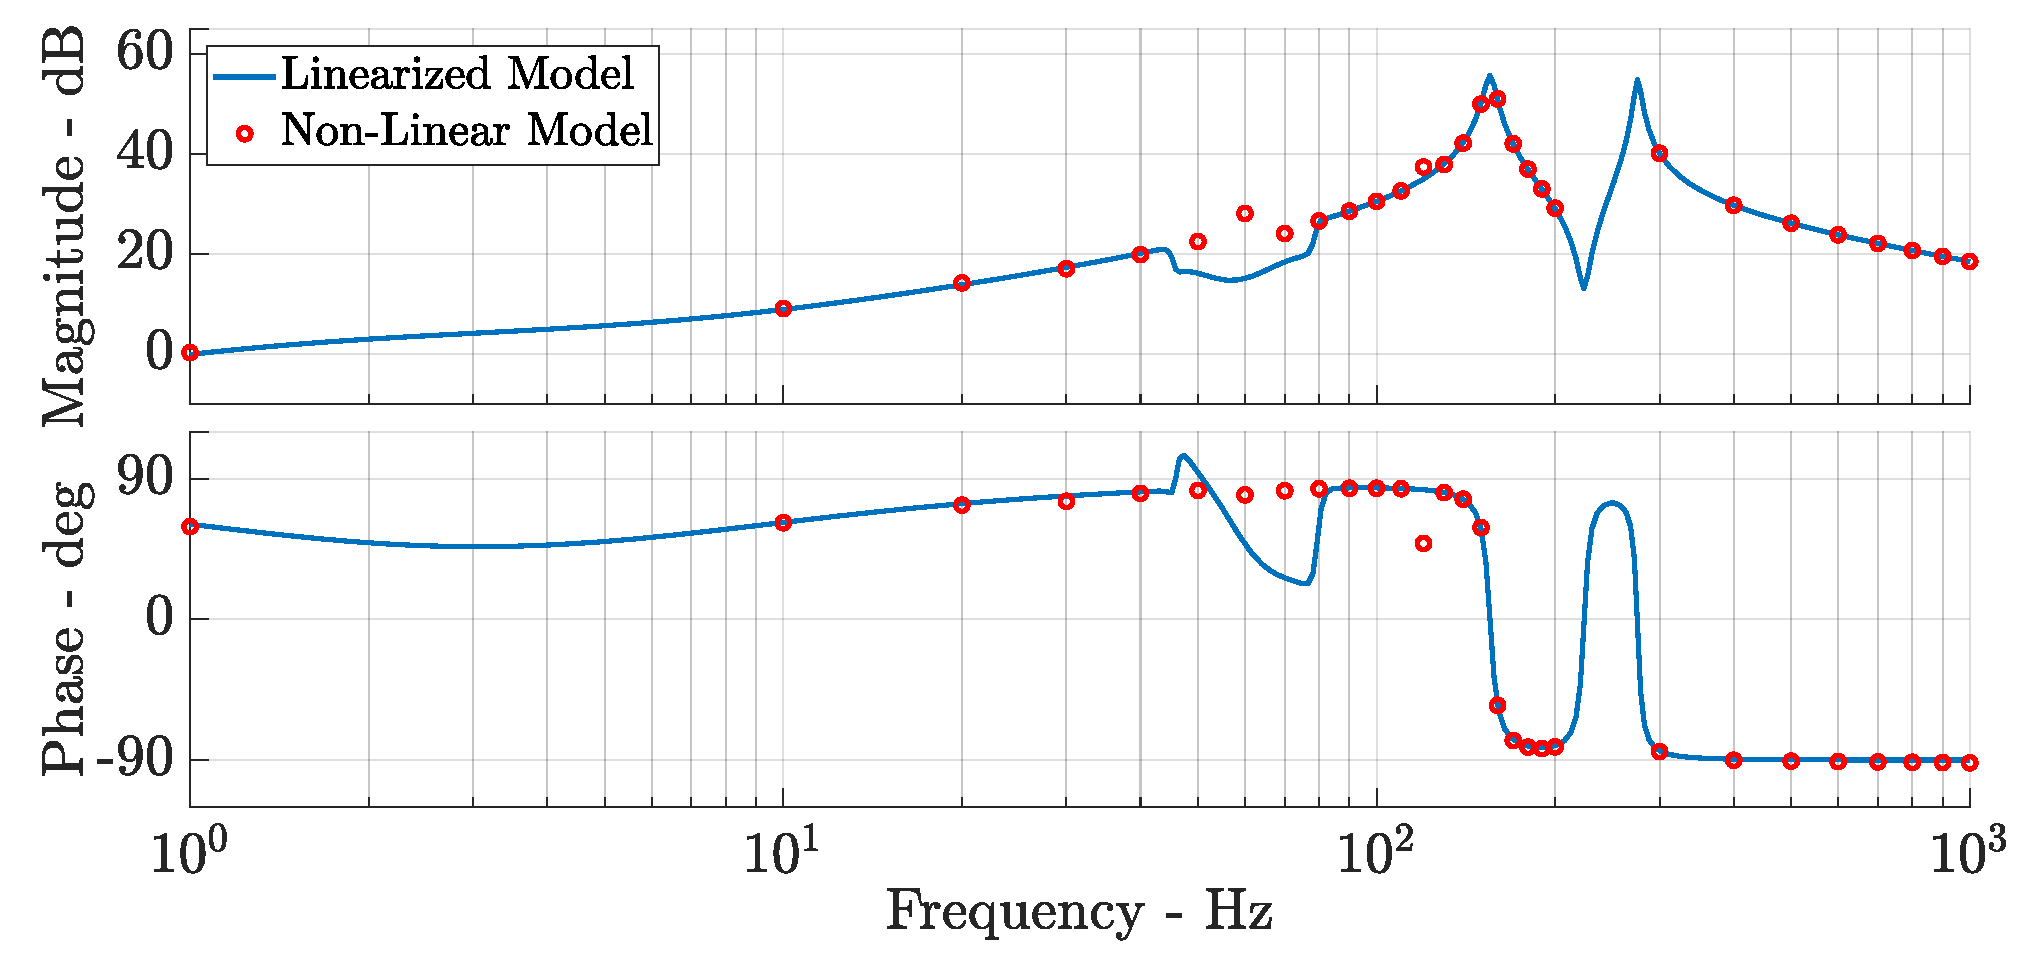
\includegraphics[width=0.60\linewidth]{./figuras/Exportacao/ex_indireto}

\end{frame}






%%%%%%%%%%%%%%%%%%%%%%%%%%%%%%%%%%%%%%%%%%%%%%%%
%%%%%%%%%%%%%%%%%%%%%%%%%%%%%%%%%%%%%%%%%%%%%%%%
%%%%%%%%%%%%%%%%%%%%%%%%%%%%%%%%%%%%%%%%%%%%%%%%
%%%%%%%%%%%%%%%%%%%%%%%%%%%%%%%%%%%%%%%%%%%%%%%%
\begin{frame}{Porque Exportar Dados?}
\centering


\textbf{Motivo 3:} Para Processar Dados
\vspace*{0.5cm}

\textbf{Ex:} Extração de componentes simétricas no domínio do tempo\footnote[frame]{\tiny Verônica Rodrigues Feijão, \href{https://drive.google.com/file/d/1xZGZLela_iNW0KIjTQ59YyCL1-sb16IO/view}{Estudo de Localização de Faltas de Curta Duração para uma Rede de 14 Barras}. Projeto de Graduação -  UERJ, 2019.}
\vspace*{0.5cm}

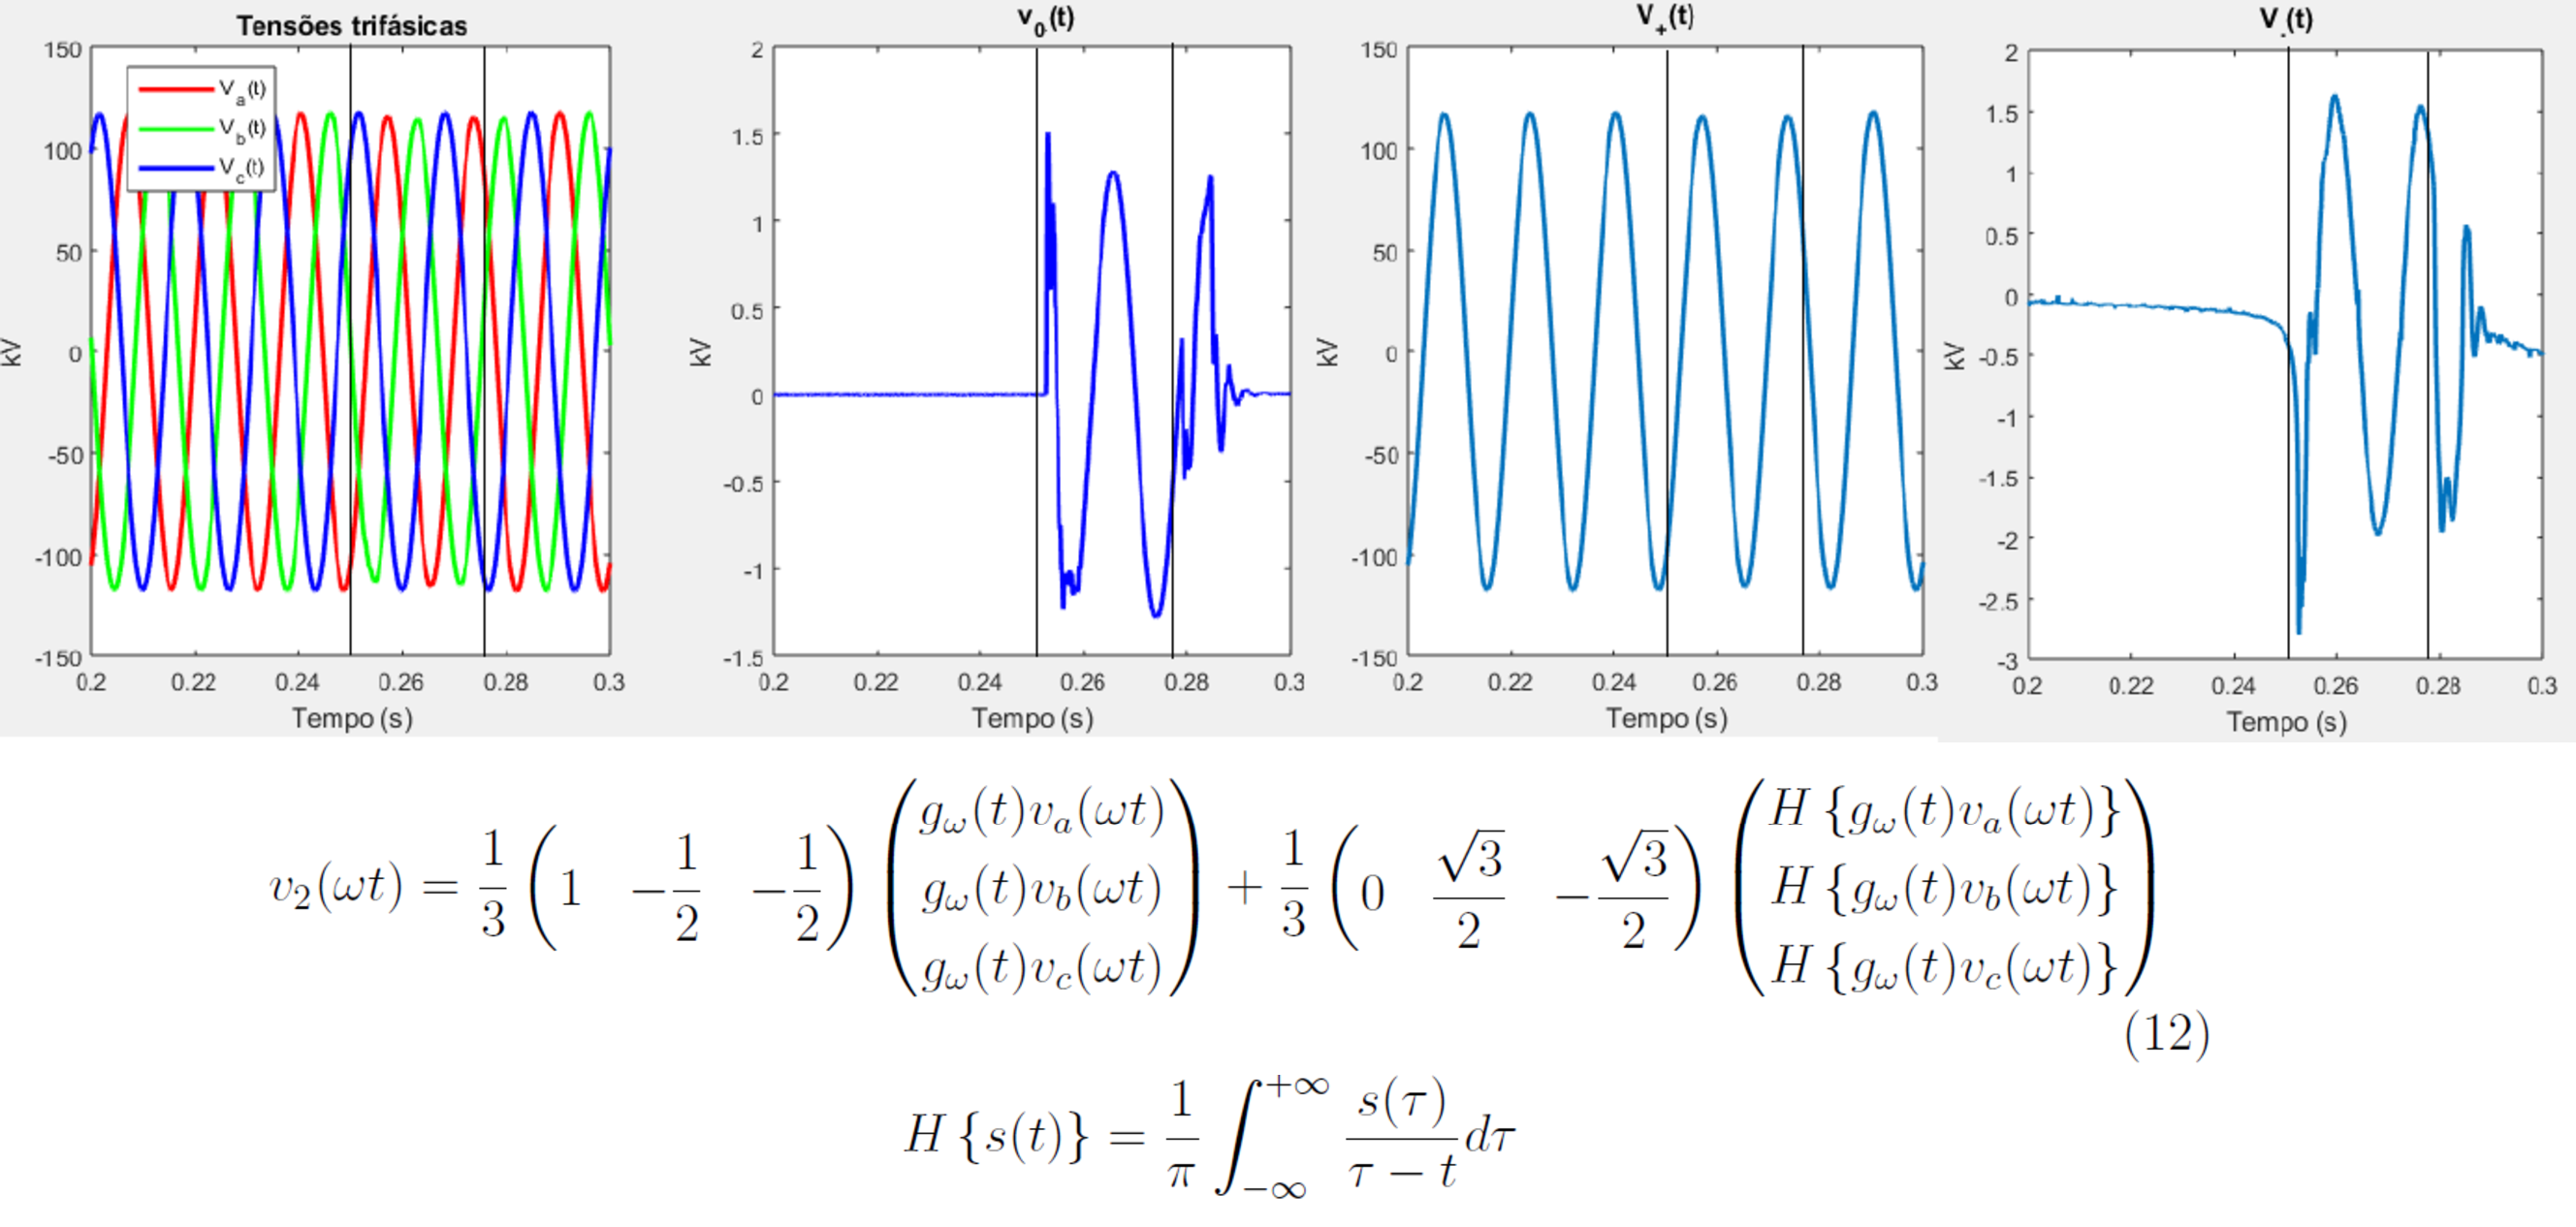
\includegraphics[width=0.65\linewidth]{./figuras/Exportacao/ex_processamento}


\end{frame}






%%%%%%%%%%%%%%%%%%%%%%%%%%%%%%%%%%%%%%%%%%%%%%%%
%%%%%%%%%%%%%%%%%%%%%%%%%%%%%%%%%%%%%%%%%%%%%%%%
%%%%%%%%%%%%%%%%%%%%%%%%%%%%%%%%%%%%%%%%%%%%%%%%
%%%%%%%%%%%%%%%%%%%%%%%%%%%%%%%%%%%%%%%%%%%%%%%%
\begin{frame}{Primeira Possibilidade: Serve para Pequenas Tarefas}
\centering

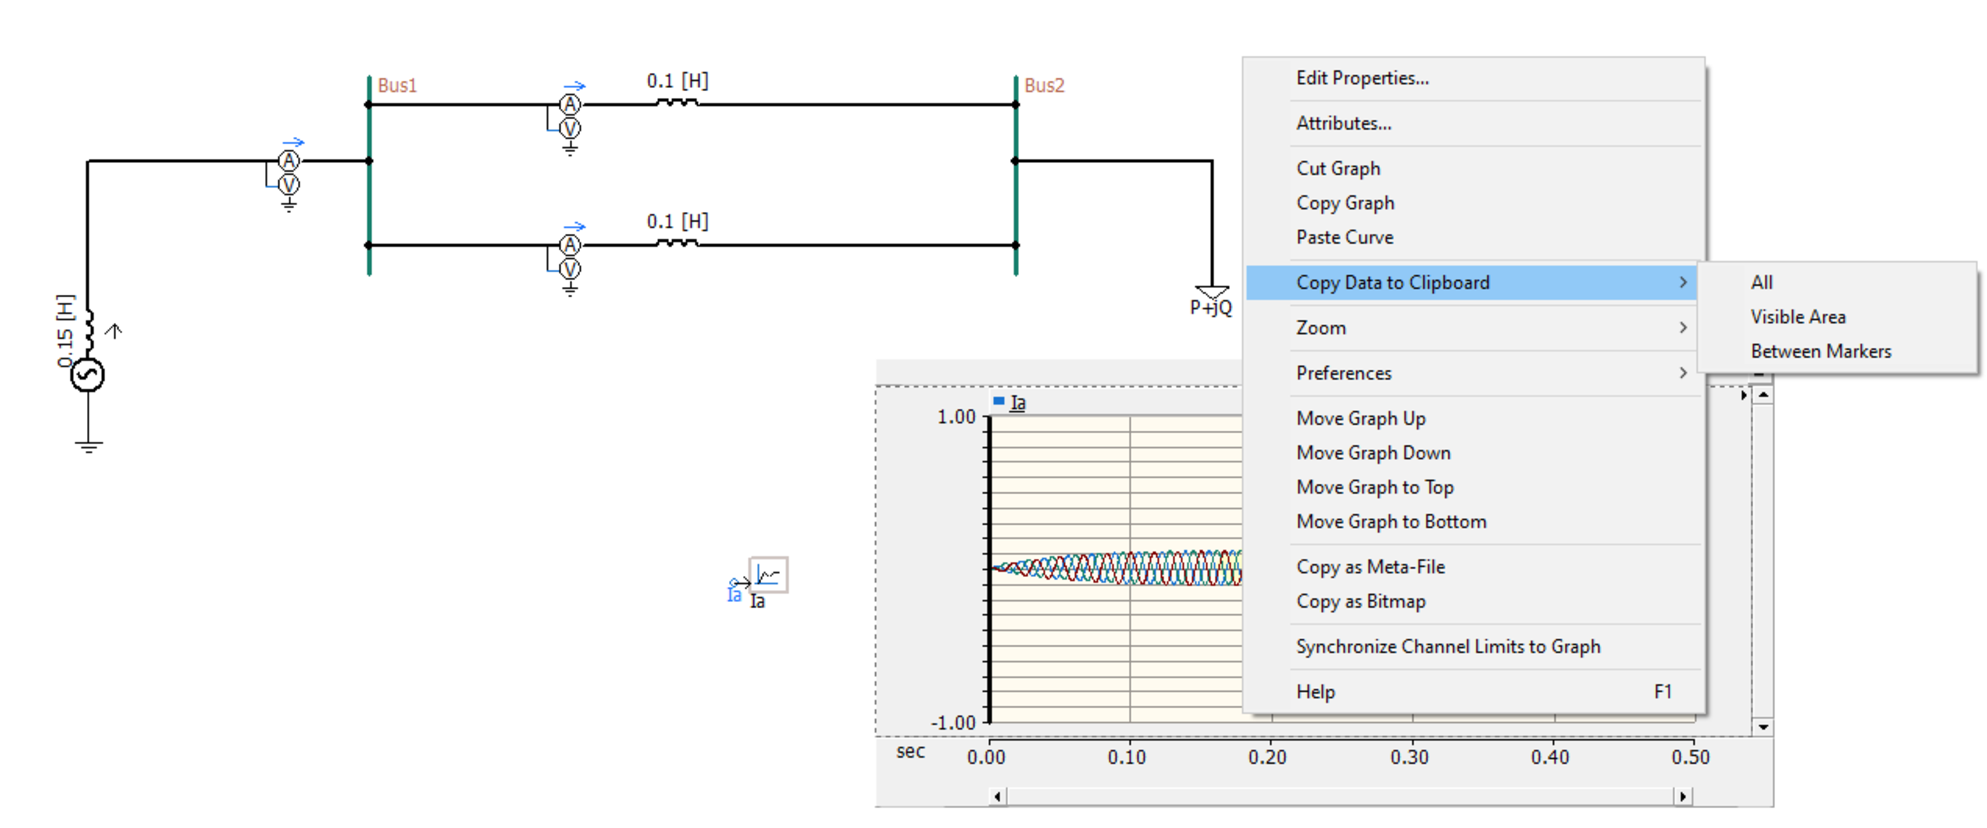
\includegraphics[width=0.95\linewidth]{./figuras/Exportacao/Export1}



\end{frame}




%%%%%%%%%%%%%%%%%%%%%%%%%%%%%%%%%%%%%%%%%%%%%%%%
%%%%%%%%%%%%%%%%%%%%%%%%%%%%%%%%%%%%%%%%%%%%%%%%
%%%%%%%%%%%%%%%%%%%%%%%%%%%%%%%%%%%%%%%%%%%%%%%%
%%%%%%%%%%%%%%%%%%%%%%%%%%%%%%%%%%%%%%%%%%%%%%%%
\begin{frame}{Primeira Possibilidade: Serve para Pequenas Tarefas}
\centering

É só colar em um arquivo de texto:

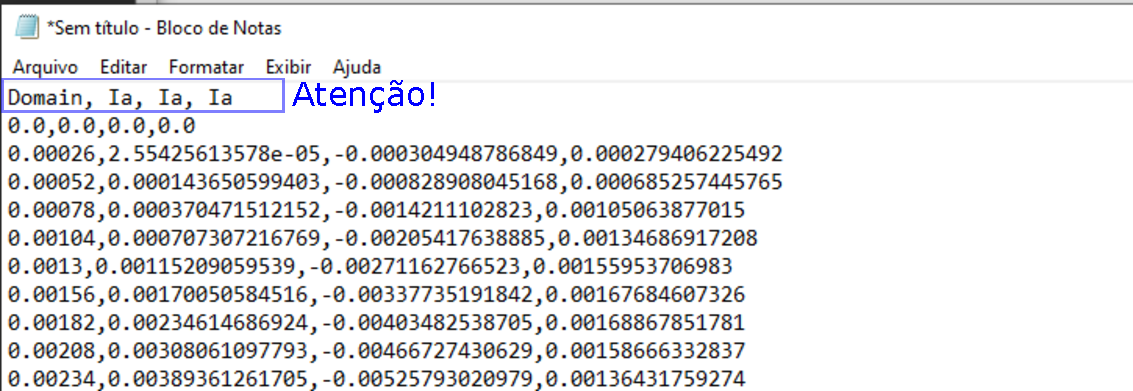
\includegraphics[width=0.95\linewidth]{./figuras/Exportacao/Export1-arquivo}



\end{frame}







%%%%%%%%%%%%%%%%%%%%%%%%%%%%%%%%%%%%%%%%%%%%%%%%
%%%%%%%%%%%%%%%%%%%%%%%%%%%%%%%%%%%%%%%%%%%%%%%%
%%%%%%%%%%%%%%%%%%%%%%%%%%%%%%%%%%%%%%%%%%%%%%%%
%%%%%%%%%%%%%%%%%%%%%%%%%%%%%%%%%%%%%%%%%%%%%%%%
\begin{frame}{Segunda Possibilidade: Útil para Grandes Tarefas}
\centering


\begin{columns}

\column{0.5\linewidth}
\begin{itemize}
\item Podemos configurar a simulação para salvar os dados dos {\i output chanels}
\vspace*{0.5cm}
\item Basta configurar a opção {\it save to disk}
\vspace*{0.5cm}
\item É gerado um arquivo com extensão {\color{blue}\it .map} contendo informações
\vspace*{0.5cm}
\item São gerados aquivos com extensão {\color{blue}\it .out} contendo os dados
\end{itemize}

\column{0.5\linewidth}
\centering
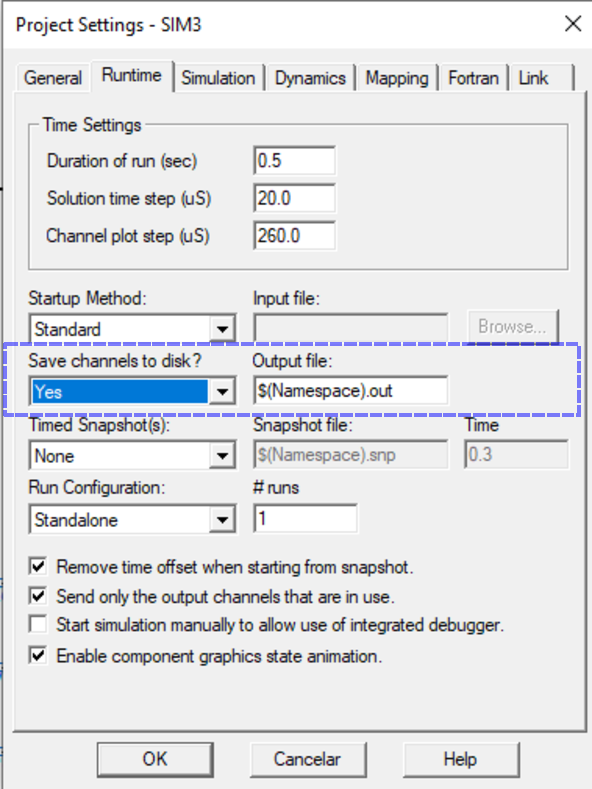
\includegraphics[width=0.70\linewidth]{./figuras/Exportacao/Export2}

\end{columns}


\end{frame}







%%%%%%%%%%%%%%%%%%%%%%%%%%%%%%%%%%%%%%%%%%%%%%%%
%%%%%%%%%%%%%%%%%%%%%%%%%%%%%%%%%%%%%%%%%%%%%%%%
%%%%%%%%%%%%%%%%%%%%%%%%%%%%%%%%%%%%%%%%%%%%%%%%
%%%%%%%%%%%%%%%%%%%%%%%%%%%%%%%%%%%%%%%%%%%%%%%%
\begin{frame}{Segunda Possibilidade: Útil para Grandes Tarefas}
\centering


\begin{columns}

\column{0.5\linewidth}
\begin{itemize}
\item Os arquivos {\color{blue}\it .out} e {\color{blue}\it .map} são dispostos na pasta de arquivos compilados da simulação
\vspace*{1cm}
\item Cada arquivo {\color{blue}\it .out} têm até 10 sinais, um por coluna
\vspace*{1cm}
\item A primeira coluna de todos os arquivos {\color{blue}\it .out} contém o vetor de domínio (Tempo ou Frequência)  
\end{itemize}

\column{0.5\linewidth}
\centering
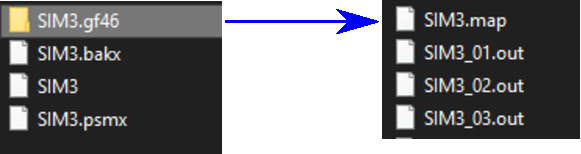
\includegraphics[width=0.70\linewidth]{./figuras/Exportacao/Export2-files}


\end{columns}


\end{frame}






%%%%%%%%%%%%%%%%%%%%%%%%%%%%%%%%%%%%%%%%%%%%%%%%
%%%%%%%%%%%%%%%%%%%%%%%%%%%%%%%%%%%%%%%%%%%%%%%%
%%%%%%%%%%%%%%%%%%%%%%%%%%%%%%%%%%%%%%%%%%%%%%%%
%%%%%%%%%%%%%%%%%%%%%%%%%%%%%%%%%%%%%%%%%%%%%%%%
\begin{frame}{Segunda Possibilidade: Útil para Grandes Tarefas}
\centering


\begin{columns}

\column{0.5\linewidth}
\centering
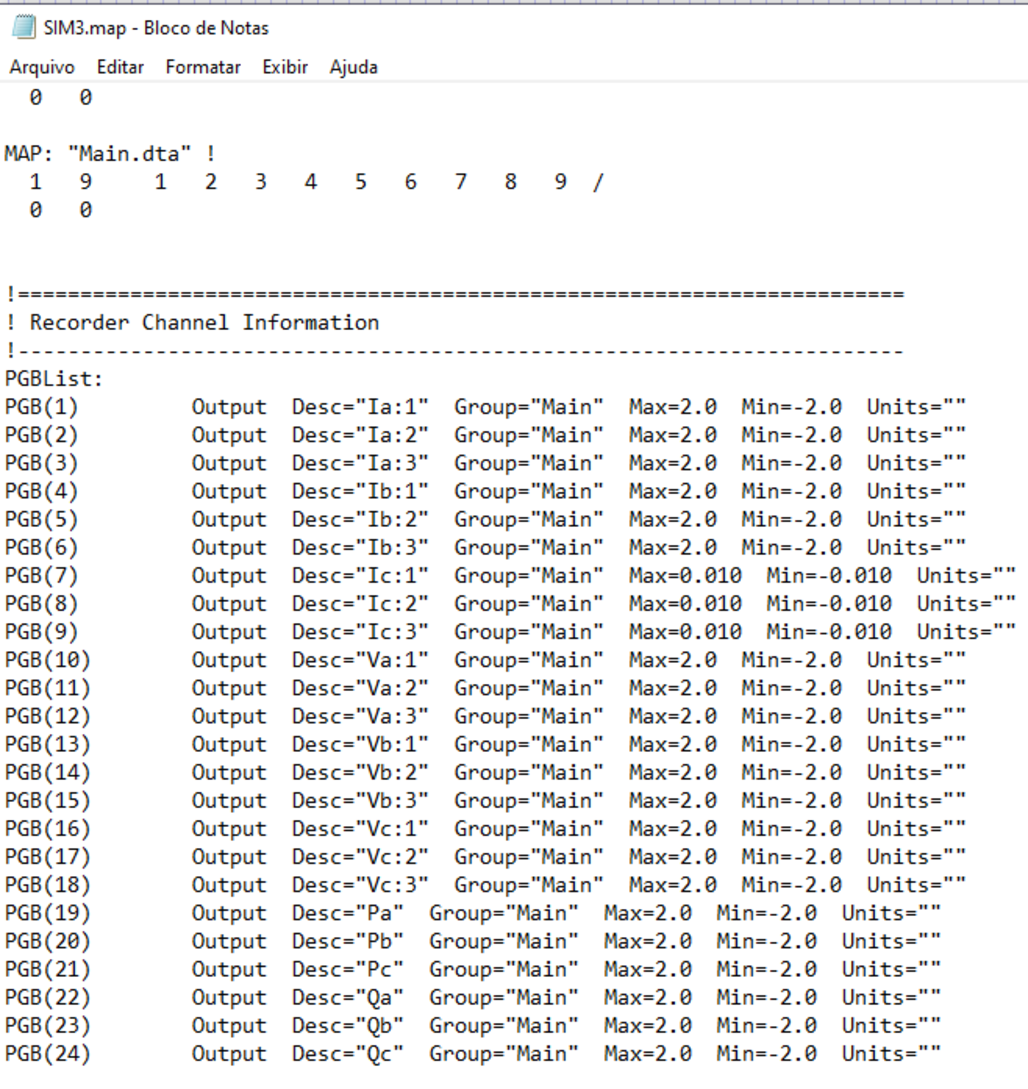
\includegraphics[width=0.80\linewidth]{./figuras/Exportacao/Export2-map}

\column{0.5\linewidth}
\centering
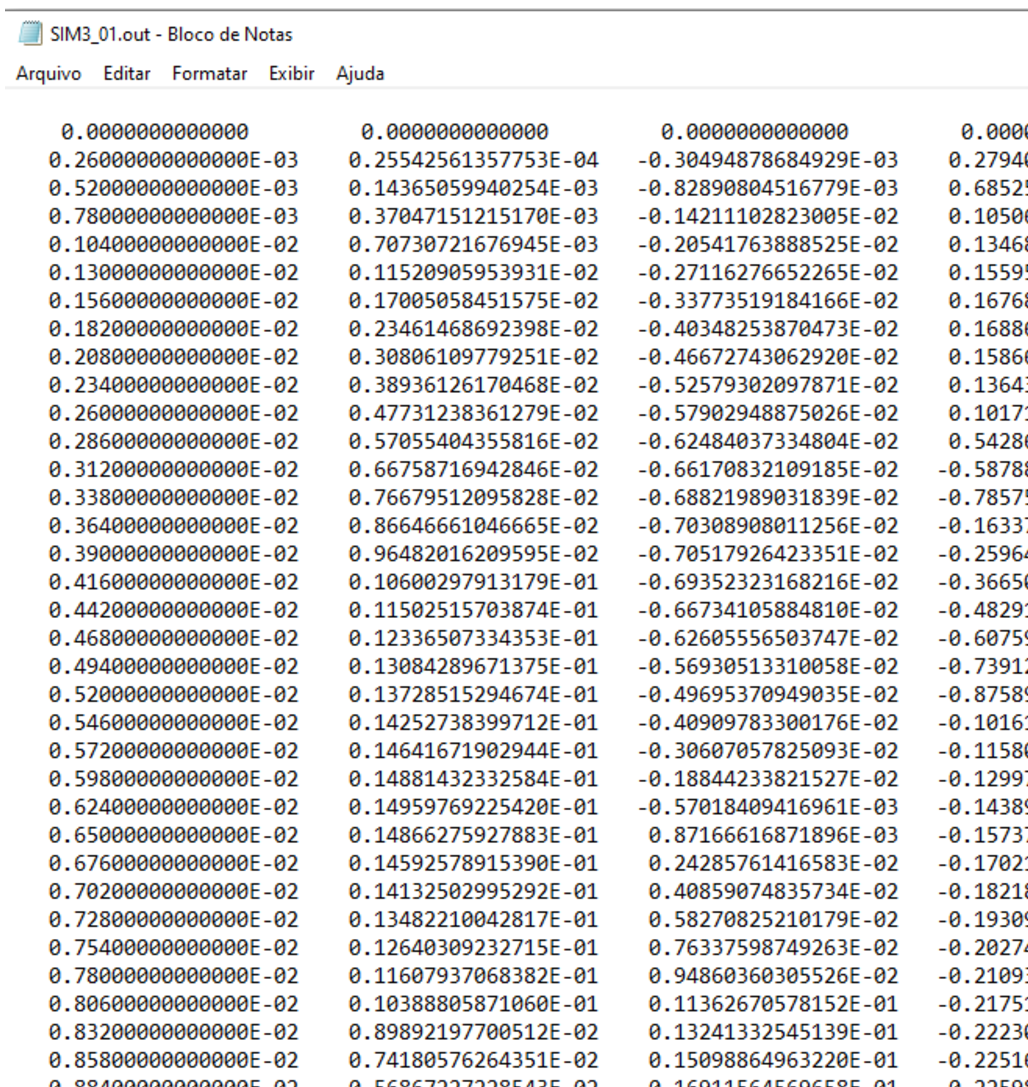
\includegraphics[width=0.80\linewidth]{./figuras/Exportacao/Export2-out}


\end{columns}


\end{frame}



\cmfnewsection{Automação de Simulações}{./logos/fundo_tese}{0.15}





%%%%%%%%%%%%%%%%%%%%%%%%%%%%%%%%%%%%%%%%%%%%%%%%
%%%%%%%%%%%%%%%%%%%%%%%%%%%%%%%%%%%%%%%%%%%%%%%%
%%%%%%%%%%%%%%%%%%%%%%%%%%%%%%%%%%%%%%%%%%%%%%%%
%%%%%%%%%%%%%%%%%%%%%%%%%%%%%%%%%%%%%%%%%%%%%%%%
\begin{frame}{O que significa automatizar simulações?}
\centering


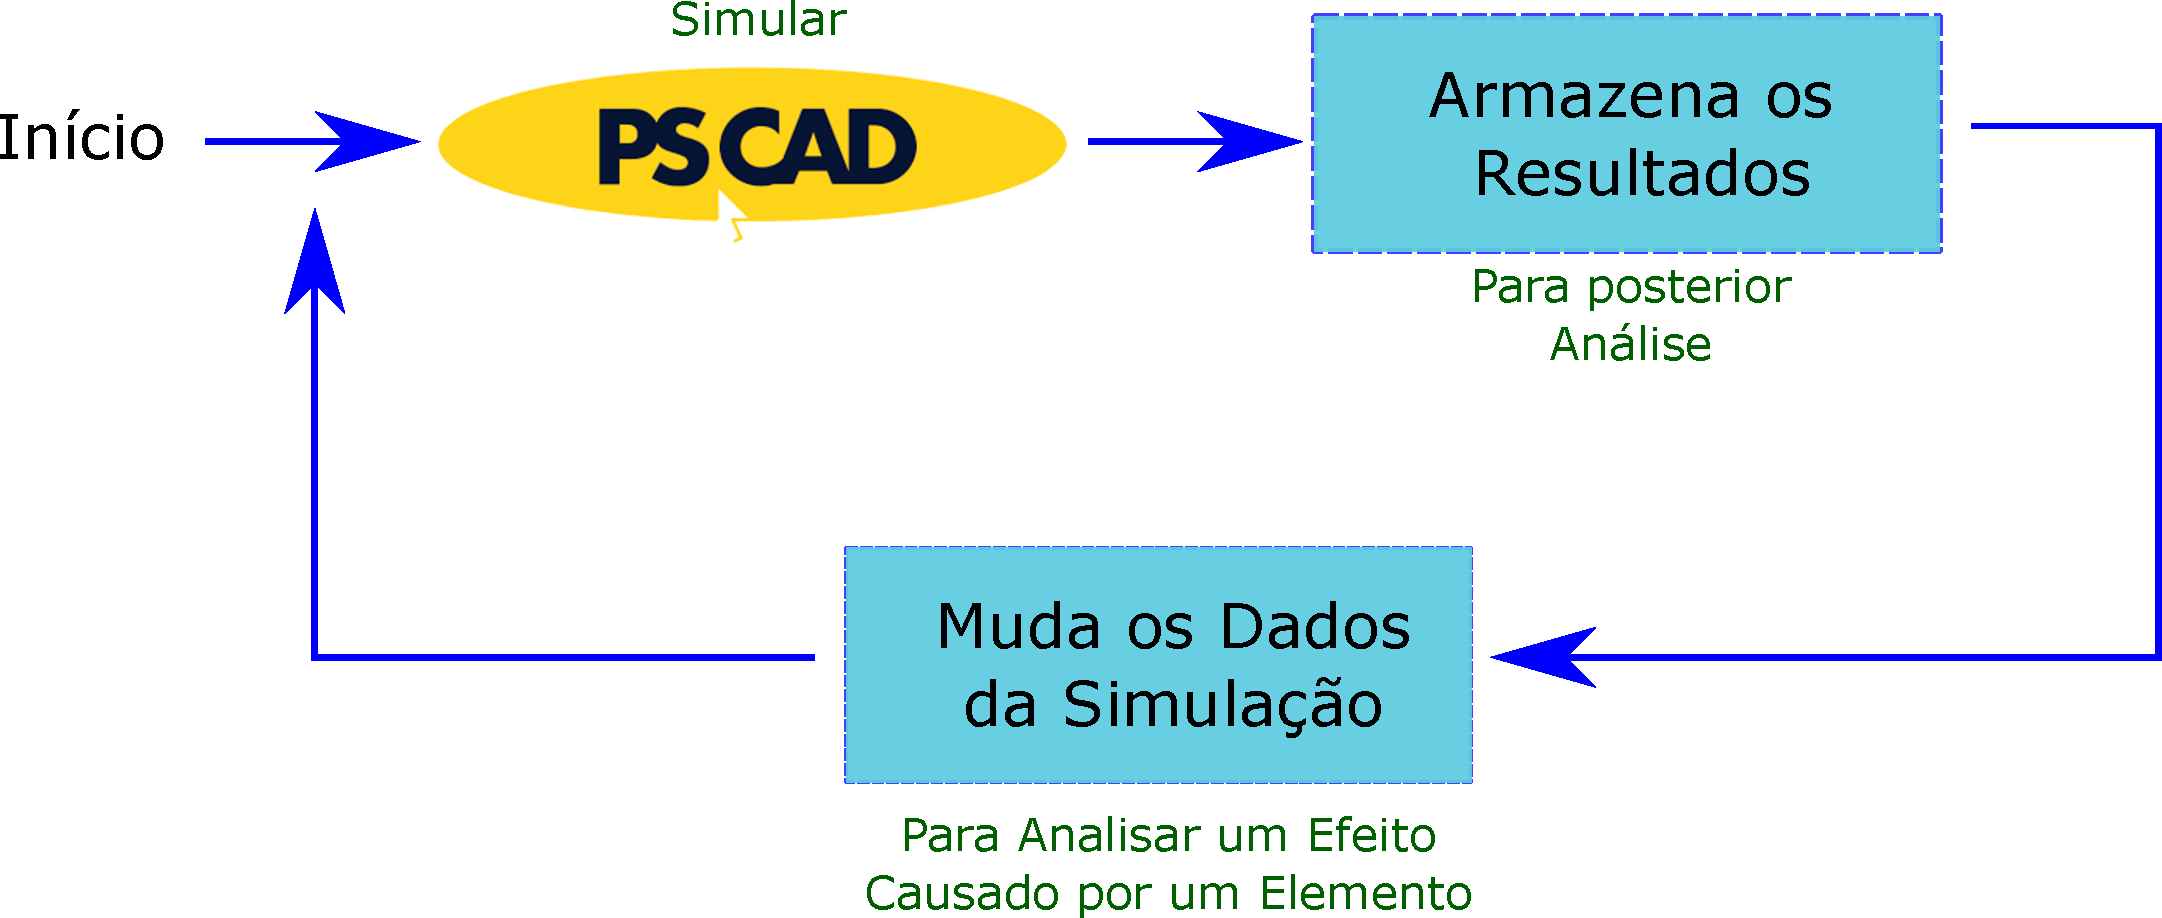
\includegraphics[width=0.80\linewidth]{./figuras/Automacao/automa}


\end{frame}





%%%%%%%%%%%%%%%%%%%%%%%%%%%%%%%%%%%%%%%%%%%%%%%%
%%%%%%%%%%%%%%%%%%%%%%%%%%%%%%%%%%%%%%%%%%%%%%%%
%%%%%%%%%%%%%%%%%%%%%%%%%%%%%%%%%%%%%%%%%%%%%%%%
%%%%%%%%%%%%%%%%%%%%%%%%%%%%%%%%%%%%%%%%%%%%%%%%
\begin{frame}{Por que automatizar simulações?}
\centering

\textbf{Motivo 1:} Ajustar sistemas de controle
\vspace*{0.5cm}

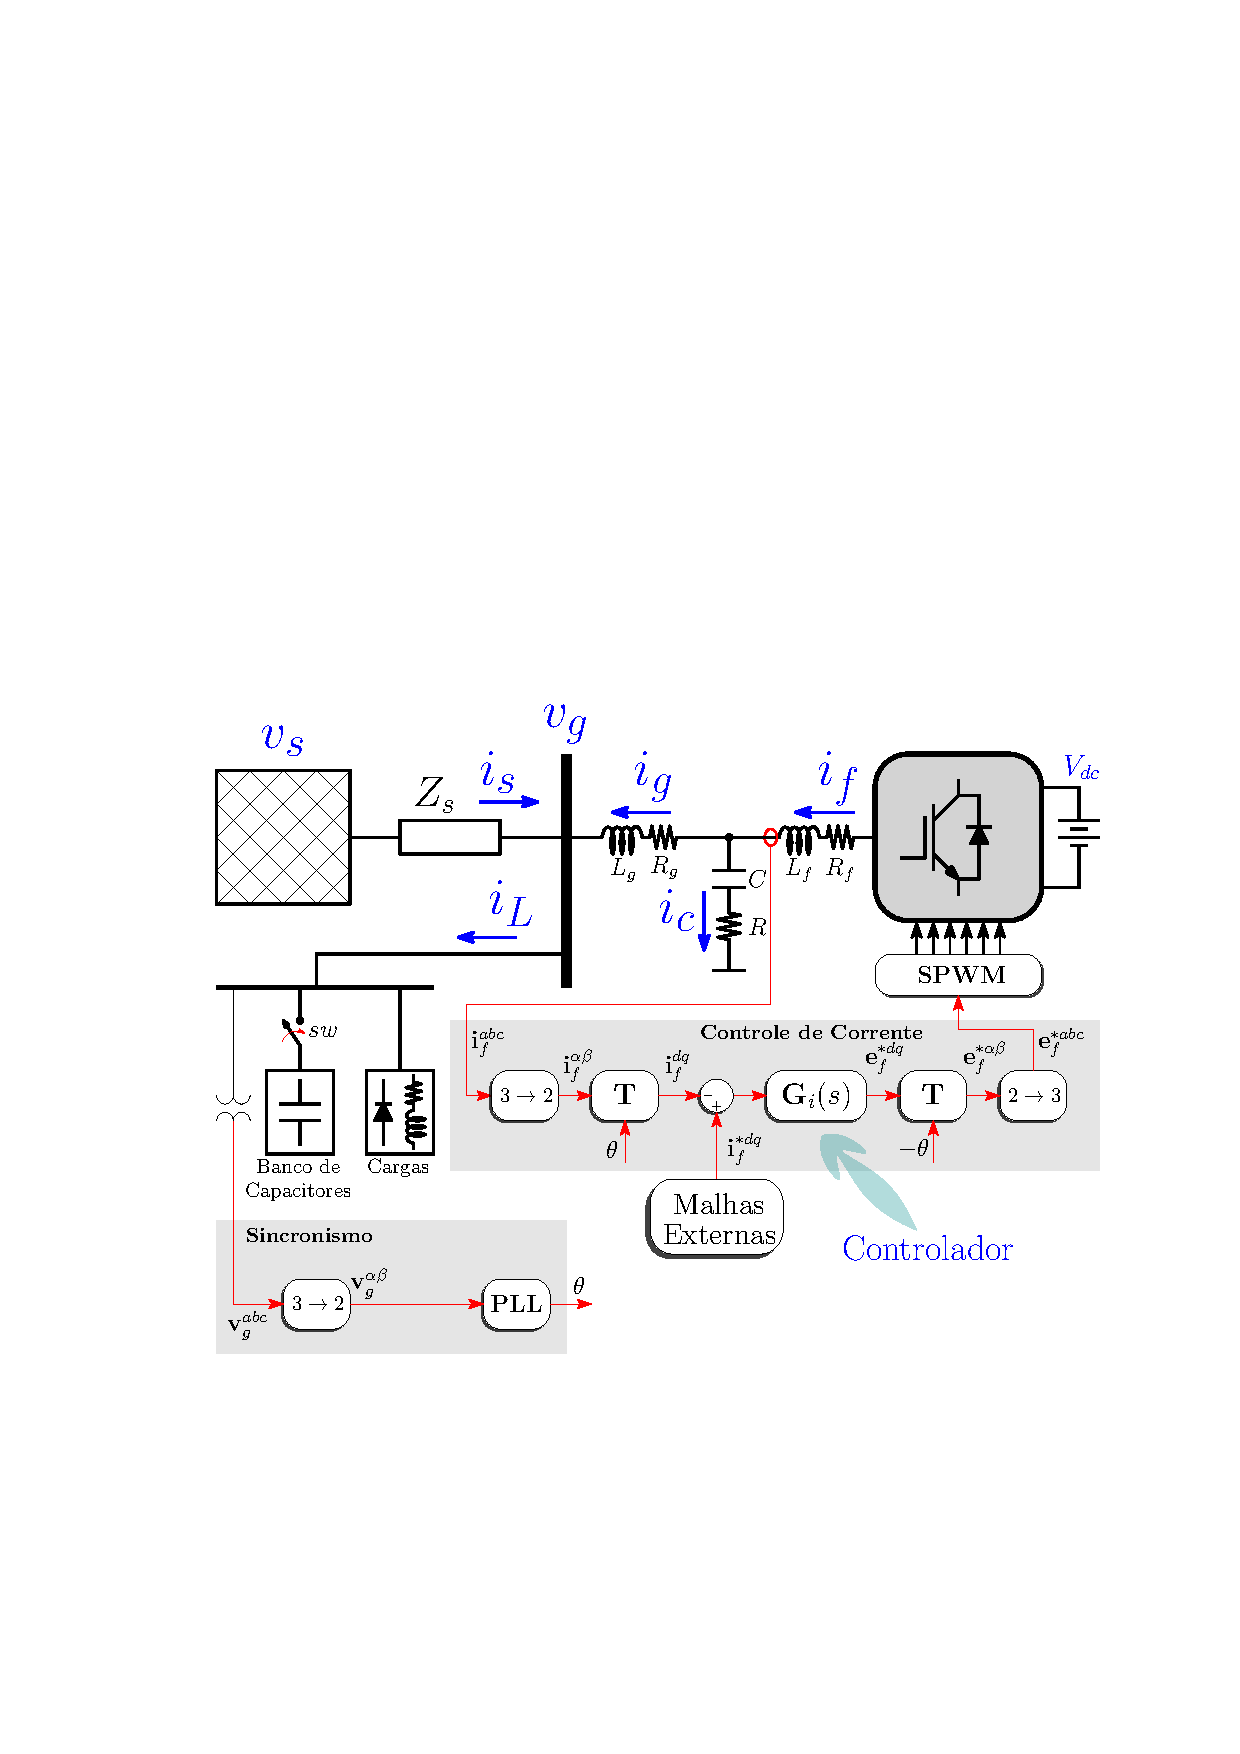
\includegraphics[width=0.55\linewidth]{./figuras/Automacao/SISTEMA}

\end{frame}







%%%%%%%%%%%%%%%%%%%%%%%%%%%%%%%%%%%%%%%%%%%%%%%%
%%%%%%%%%%%%%%%%%%%%%%%%%%%%%%%%%%%%%%%%%%%%%%%%
%%%%%%%%%%%%%%%%%%%%%%%%%%%%%%%%%%%%%%%%%%%%%%%%
%%%%%%%%%%%%%%%%%%%%%%%%%%%%%%%%%%%%%%%%%%%%%%%%
\begin{frame}{Por que automatizar simulações?}
\centering

\textbf{Motivo 2:} Avaliar efeitos de eventos em diferentes pontos em um sistema grande\footnote[frame]{\tiny Verônica Rodrigues Feijão, \href{https://drive.google.com/file/d/1xZGZLela_iNW0KIjTQ59YyCL1-sb16IO/view}{Estudo de Localização de Faltas de Curta Duração para uma Rede de 14 Barras}. Projeto de Graduação -  UERJ, 2019.}
%\vspace*{1cm}

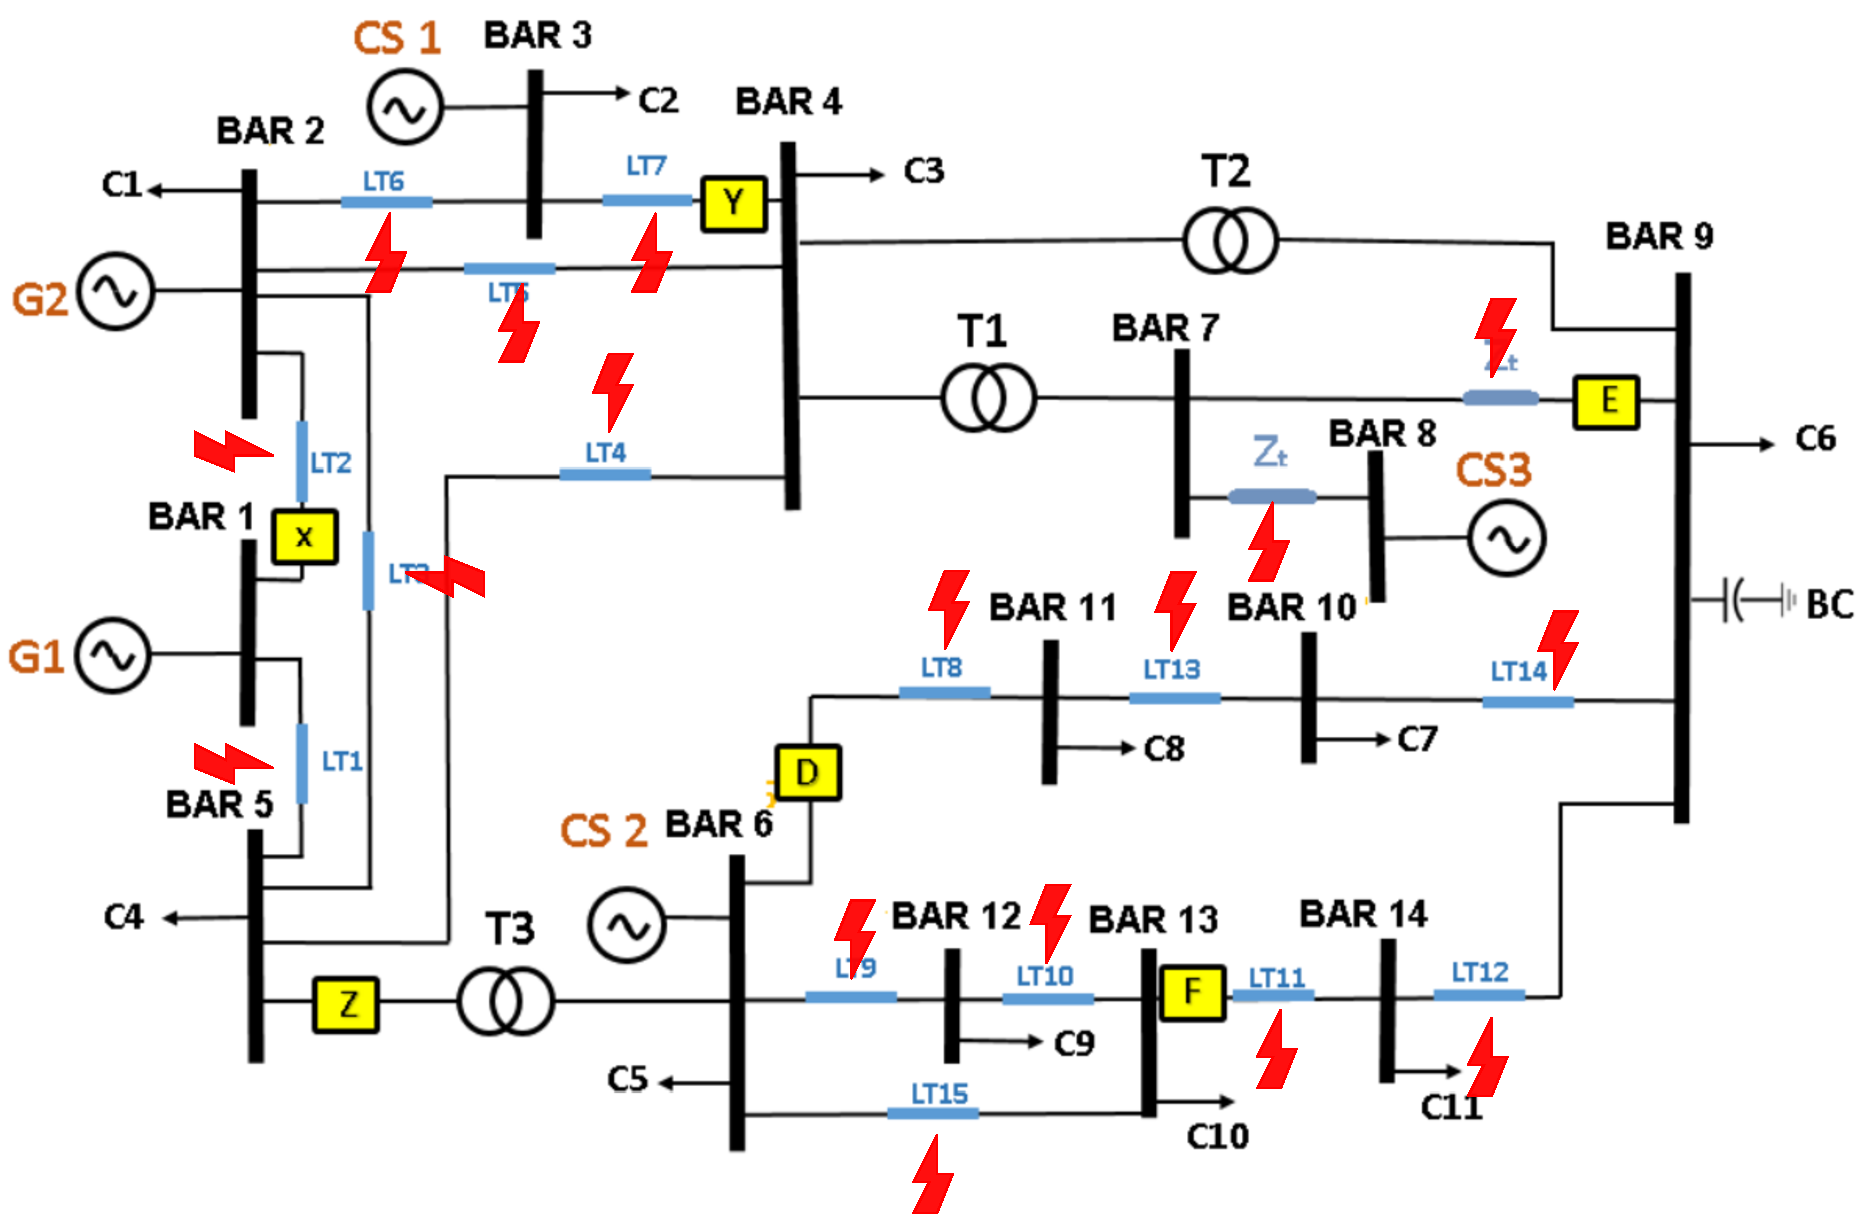
\includegraphics[width=0.6\linewidth]{./figuras/Automacao/ex_curto}

\end{frame}





%%%%%%%%%%%%%%%%%%%%%%%%%%%%%%%%%%%%%%%%%%%%%%%%
%%%%%%%%%%%%%%%%%%%%%%%%%%%%%%%%%%%%%%%%%%%%%%%%
%%%%%%%%%%%%%%%%%%%%%%%%%%%%%%%%%%%%%%%%%%%%%%%%
%%%%%%%%%%%%%%%%%%%%%%%%%%%%%%%%%%%%%%%%%%%%%%%%
\begin{frame}{Como fazer?}
\centering

\begin{columns}


\column{0.5\linewidth}

\begin{itemize}
\item Inserir/Configurar o bloco {\it Multiple run} localizado no grupo de {\it I/O Devices} na biblioteca Master.

\vspace*{2.5cm}

\item Configurar o projeto para {\it Multiple run}.

\vspace*{1cm}
\end{itemize}


\column{0.5\linewidth}
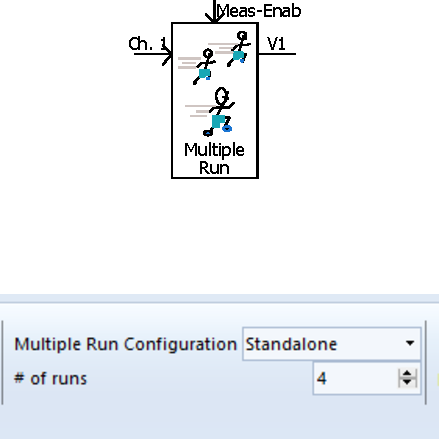
\includegraphics[width=0.80\linewidth]{./figuras/Automacao/multrun}

\end{columns}

\end{frame}




%%%%%%%%%%%%%%%%%%%%%%%%%%%%%%%%%%%%%%%%%%%%%%%%
%%%%%%%%%%%%%%%%%%%%%%%%%%%%%%%%%%%%%%%%%%%%%%%%
%%%%%%%%%%%%%%%%%%%%%%%%%%%%%%%%%%%%%%%%%%%%%%%%
%%%%%%%%%%%%%%%%%%%%%%%%%%%%%%%%%%%%%%%%%%%%%%%%
\begin{frame}{Circuito Exemplo}
\centering

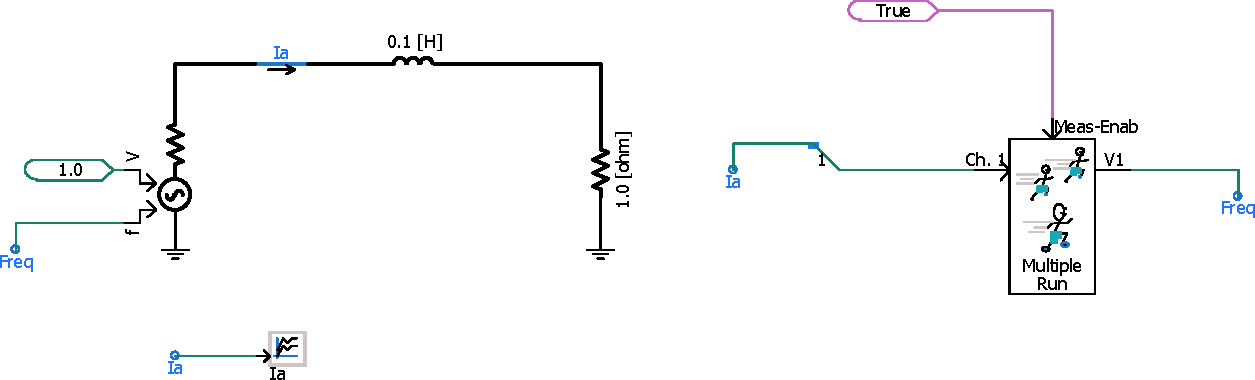
\includegraphics[width=0.85\linewidth]{./figuras/Automacao/SIM}

\end{frame}


%\cmfnewsection{Criação de Componentes e Bibliotecas}{./logos/fundo_tese}{0.15}







%%%%%%%%%%%%%%%%%%%%%%%%%%%%%%%%%%%%%%%%%%%%%%%%
%%%%%%%%%%%%%%%%%%%%%%%%%%%%%%%%%%%%%%%%%%%%%%%%
%%%%%%%%%%%%%%%%%%%%%%%%%%%%%%%%%%%%%%%%%%%%%%%%
%%%%%%%%%%%%%%%%%%%%%%%%%%%%%%%%%%%%%%%%%%%%%%%%
\begin{frame}{Encapsulando Circuitos: {\it Component Wizard}}
\centering


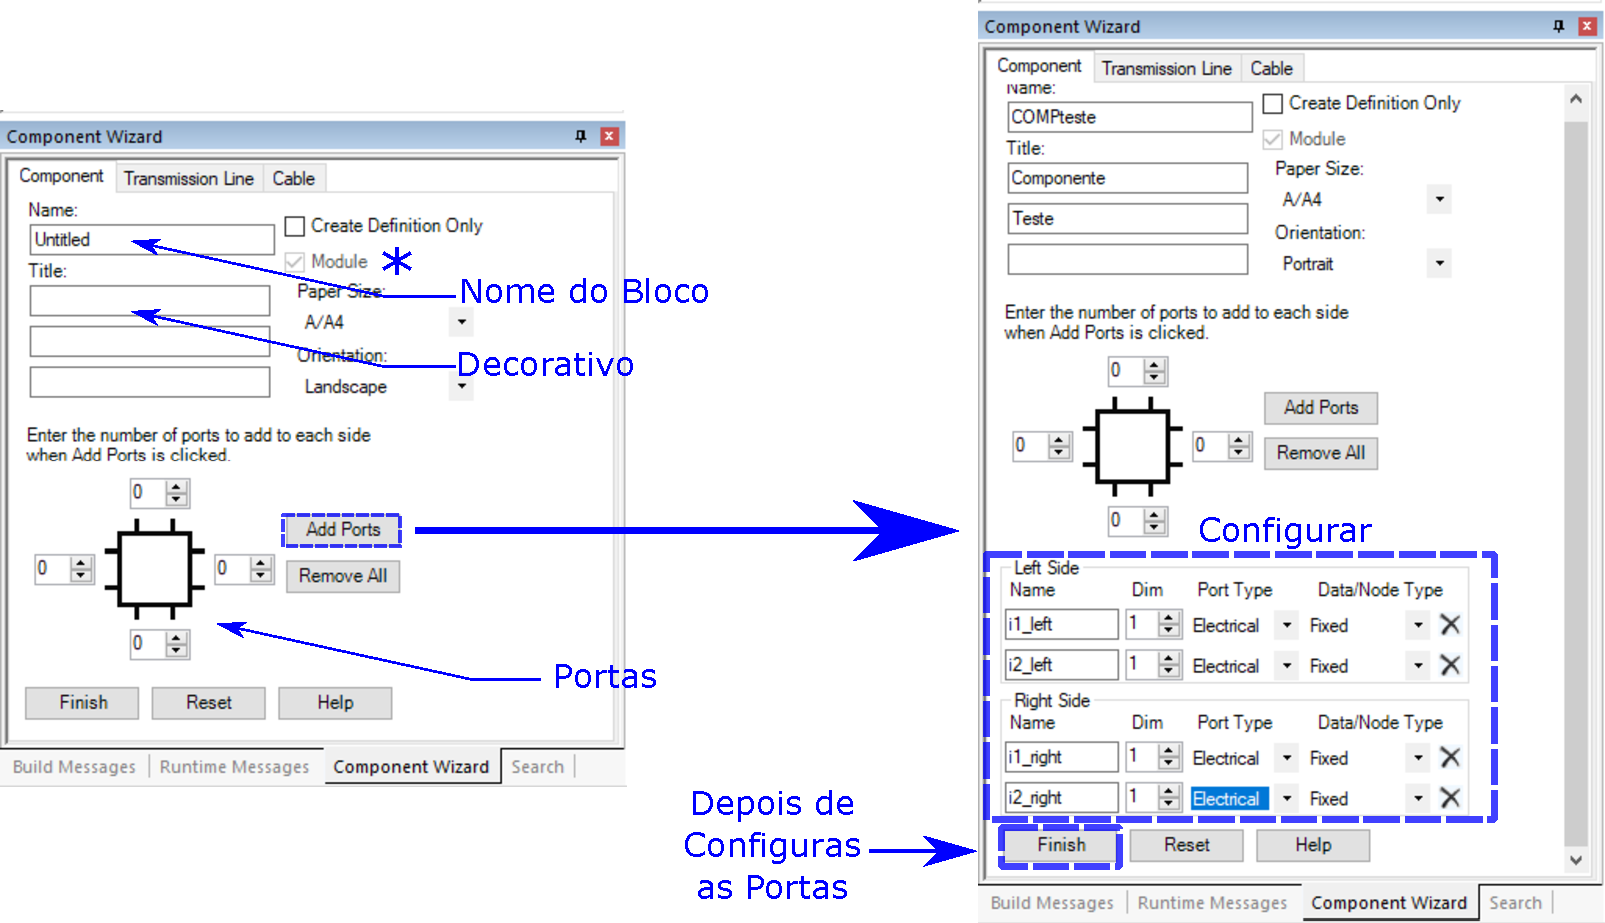
\includegraphics[width=0.75\linewidth]{./figuras/Componentes/wizard}


\end{frame}





%%%%%%%%%%%%%%%%%%%%%%%%%%%%%%%%%%%%%%%%%%%%%%%%
%%%%%%%%%%%%%%%%%%%%%%%%%%%%%%%%%%%%%%%%%%%%%%%%
%%%%%%%%%%%%%%%%%%%%%%%%%%%%%%%%%%%%%%%%%%%%%%%%
%%%%%%%%%%%%%%%%%%%%%%%%%%%%%%%%%%%%%%%%%%%%%%%%
\begin{frame}{Encapsulando Circuitos: Resultado}
\centering


\includegraphics[width=0.45\linewidth]{./figuras/Componentes/componenteTeste}


\end{frame}




%%%%%%%%%%%%%%%%%%%%%%%%%%%%%%%%%%%%%%%%%%%%%%%%
%%%%%%%%%%%%%%%%%%%%%%%%%%%%%%%%%%%%%%%%%%%%%%%%
%%%%%%%%%%%%%%%%%%%%%%%%%%%%%%%%%%%%%%%%%%%%%%%%
%%%%%%%%%%%%%%%%%%%%%%%%%%%%%%%%%%%%%%%%%%%%%%%%
\begin{frame}{Encapsulando Circuitos: Montando o Esquemático}
\centering


\includegraphics[width=0.75\linewidth]{./figuras/Componentes/schematico}


\end{frame}







%%%%%%%%%%%%%%%%%%%%%%%%%%%%%%%%%%%%%%%%%%%%%%%%
%%%%%%%%%%%%%%%%%%%%%%%%%%%%%%%%%%%%%%%%%%%%%%%%
%%%%%%%%%%%%%%%%%%%%%%%%%%%%%%%%%%%%%%%%%%%%%%%%
%%%%%%%%%%%%%%%%%%%%%%%%%%%%%%%%%%%%%%%%%%%%%%%%
\begin{frame}{Encapsulando Circuitos: Testando}
\centering


\includegraphics[width=0.75\linewidth]{./figuras/Componentes/Testando}


\end{frame}






%%%%%%%%%%%%%%%%%%%%%%%%%%%%%%%%%%%%%%%%%%%%%%%%
%%%%%%%%%%%%%%%%%%%%%%%%%%%%%%%%%%%%%%%%%%%%%%%%
%%%%%%%%%%%%%%%%%%%%%%%%%%%%%%%%%%%%%%%%%%%%%%%%
%%%%%%%%%%%%%%%%%%%%%%%%%%%%%%%%%%%%%%%%%%%%%%%%
\begin{frame}{Encapsulando Circuitos: {\it Decorando o Bloco}}
\centering


\includegraphics[width=0.75\linewidth]{./figuras/Componentes/grafica}


\end{frame}






%%%%%%%%%%%%%%%%%%%%%%%%%%%%%%%%%%%%%%%%%%%%%%%%
%%%%%%%%%%%%%%%%%%%%%%%%%%%%%%%%%%%%%%%%%%%%%%%%
%%%%%%%%%%%%%%%%%%%%%%%%%%%%%%%%%%%%%%%%%%%%%%%%
%%%%%%%%%%%%%%%%%%%%%%%%%%%%%%%%%%%%%%%%%%%%%%%%
\begin{frame}{Encapsulando Circuitos: Testando, de novo}
\centering


\includegraphics[width=0.75\linewidth]{./figuras/Componentes/Testando2}


\end{frame}




%%%%%%%%%%%%%%%%%%%%%%%%%%%%%%%%%%%%%%%%%%%%%%%%
%%%%%%%%%%%%%%%%%%%%%%%%%%%%%%%%%%%%%%%%%%%%%%%%
%%%%%%%%%%%%%%%%%%%%%%%%%%%%%%%%%%%%%%%%%%%%%%%%
%%%%%%%%%%%%%%%%%%%%%%%%%%%%%%%%%%%%%%%%%%%%%%%%
\begin{frame}{Programando componentes com FORTRAN}
\centering

\begin{columns}


\column{0.5\linewidth}
\begin{itemize}
\item Criar um bloco seguindo os passos anteriores
\vspace*{1cm}
\item Demarcar a opção {\it Module}
\vspace*{1cm}
\item Programar o bloco na aba script
\end{itemize}

\column{0.5\linewidth}
\includegraphics[width=0.75\linewidth]{./figuras/Componentes/componenteFortran}

\end{columns}




\end{frame}




%%%%%%%%%%%%%%%%%%%%%%%%%%%%%%%%%%%%%%%%%%%%%%%%
%%%%%%%%%%%%%%%%%%%%%%%%%%%%%%%%%%%%%%%%%%%%%%%%
%%%%%%%%%%%%%%%%%%%%%%%%%%%%%%%%%%%%%%%%%%%%%%%%
%%%%%%%%%%%%%%%%%%%%%%%%%%%%%%%%%%%%%%%%%%%%%%%%
\begin{frame}{Programando componentes com FORTRAN: Componente A}
\centering

Componente que soma uma constante $K$ a todos os elementos de um vetor. Ou seja:
\vspace*{0.5cm}

\begin{equation*}
\mathbf{y}[n] = \mathbf{x}[n] + K 
\end{equation*}
\vspace*{0.5cm}

$\mathbf{y}$ - Vetor com $N$ posições (saída do bloco)
\vspace*{0.5cm}

$\mathbf{x}$ - Vetor com $N$ posições (entrada do bloco)
\vspace*{0.5cm}

$K$ - Constante


\end{frame}





%%%%%%%%%%%%%%%%%%%%%%%%%%%%%%%%%%%%%%%%%%%%%%%%
%%%%%%%%%%%%%%%%%%%%%%%%%%%%%%%%%%%%%%%%%%%%%%%%
%%%%%%%%%%%%%%%%%%%%%%%%%%%%%%%%%%%%%%%%%%%%%%%%
%%%%%%%%%%%%%%%%%%%%%%%%%%%%%%%%%%%%%%%%%%%%%%%%
\begin{frame}{Programando componentes com FORTRAN: Componente A}
\centering

\includegraphics[width=0.75\linewidth]{./figuras/Componentes/FortranA_parameter}

\end{frame}




%%%%%%%%%%%%%%%%%%%%%%%%%%%%%%%%%%%%%%%%%%%%%%%%
%%%%%%%%%%%%%%%%%%%%%%%%%%%%%%%%%%%%%%%%%%%%%%%%
%%%%%%%%%%%%%%%%%%%%%%%%%%%%%%%%%%%%%%%%%%%%%%%%
%%%%%%%%%%%%%%%%%%%%%%%%%%%%%%%%%%%%%%%%%%%%%%%%
\begin{frame}{Programando componentes com FORTRAN: Componente A}
\centering

\includegraphics[width=0.75\linewidth]{./figuras/Componentes/FortranA_script}

\end{frame}




%%%%%%%%%%%%%%%%%%%%%%%%%%%%%%%%%%%%%%%%%%%%%%%%
%%%%%%%%%%%%%%%%%%%%%%%%%%%%%%%%%%%%%%%%%%%%%%%%
%%%%%%%%%%%%%%%%%%%%%%%%%%%%%%%%%%%%%%%%%%%%%%%%
%%%%%%%%%%%%%%%%%%%%%%%%%%%%%%%%%%%%%%%%%%%%%%%%
\begin{frame}{Programando componentes com FORTRAN: Componente B}
\centering

\includegraphics[width=0.45\linewidth]{./figuras/Componentes/FortranB_script}

\end{frame}





%%%%%%%%%%%%%%%%%%%%%%%%%%%%%%%%%%%%%%%%%%%%%%%%
%%%%%%%%%%%%%%%%%%%%%%%%%%%%%%%%%%%%%%%%%%%%%%%%
%%%%%%%%%%%%%%%%%%%%%%%%%%%%%%%%%%%%%%%%%%%%%%%%
%%%%%%%%%%%%%%%%%%%%%%%%%%%%%%%%%%%%%%%%%%%%%%%%
\begin{frame}{Guardando componentes em uma Biblioteca}
\centering

\begin{columns}


\column{0.5\linewidth}

\begin{itemize}
\item Crie uma biblioteca
\vspace*{1cm}
\item No workspace, Copie a definição do componente do seu projeto
\vspace*{1cm}
\item Cole na seção de definições da biblioteca
\end{itemize}
\vspace*{1cm}

\column{0.5\linewidth}
\centering
\vspace*{1cm}

\includegraphics[width=0.75\linewidth]{./figuras/Componentes/lib}


\end{columns}

\end{frame}
%\cmfnewsection{Criação de Componentes: Usando Scripts}{./logos/fundo_tese}{0.15}
%\cmfnewsection{Automação de Simulações}{./logos/fundo_tese}{0.15}





%%%%%%%%%%%%%%%%%%%%%%%%%%%%%%%%%%%%%%%%%%%%%%%%
%%%%%%%%%%%%%%%%%%%%%%%%%%%%%%%%%%%%%%%%%%%%%%%%
%%%%%%%%%%%%%%%%%%%%%%%%%%%%%%%%%%%%%%%%%%%%%%%%
%%%%%%%%%%%%%%%%%%%%%%%%%%%%%%%%%%%%%%%%%%%%%%%%
\begin{frame}{O que significa automatizar simulações?}
\centering


\includegraphics[width=0.80\linewidth]{./figuras/Automacao/automa}


\end{frame}





%%%%%%%%%%%%%%%%%%%%%%%%%%%%%%%%%%%%%%%%%%%%%%%%
%%%%%%%%%%%%%%%%%%%%%%%%%%%%%%%%%%%%%%%%%%%%%%%%
%%%%%%%%%%%%%%%%%%%%%%%%%%%%%%%%%%%%%%%%%%%%%%%%
%%%%%%%%%%%%%%%%%%%%%%%%%%%%%%%%%%%%%%%%%%%%%%%%
\begin{frame}{Por que automatizar simulações?}
\centering

\textbf{Motivo 1:} Ajustar sistemas de controle
\vspace*{0.5cm}

\includegraphics[width=0.55\linewidth]{./figuras/Automacao/SISTEMA}

\end{frame}







%%%%%%%%%%%%%%%%%%%%%%%%%%%%%%%%%%%%%%%%%%%%%%%%
%%%%%%%%%%%%%%%%%%%%%%%%%%%%%%%%%%%%%%%%%%%%%%%%
%%%%%%%%%%%%%%%%%%%%%%%%%%%%%%%%%%%%%%%%%%%%%%%%
%%%%%%%%%%%%%%%%%%%%%%%%%%%%%%%%%%%%%%%%%%%%%%%%
\begin{frame}{Por que automatizar simulações?}
\centering

\textbf{Motivo 2:} Avaliar efeitos de eventos em diferentes pontos em um sistema grande\footnote[frame]{\tiny Verônica Rodrigues Feijão, \href{https://drive.google.com/file/d/1xZGZLela_iNW0KIjTQ59YyCL1-sb16IO/view}{Estudo de Localização de Faltas de Curta Duração para uma Rede de 14 Barras}. Projeto de Graduação -  UERJ, 2019.}
%\vspace*{1cm}

\includegraphics[width=0.6\linewidth]{./figuras/Automacao/ex_curto}

\end{frame}





%%%%%%%%%%%%%%%%%%%%%%%%%%%%%%%%%%%%%%%%%%%%%%%%
%%%%%%%%%%%%%%%%%%%%%%%%%%%%%%%%%%%%%%%%%%%%%%%%
%%%%%%%%%%%%%%%%%%%%%%%%%%%%%%%%%%%%%%%%%%%%%%%%
%%%%%%%%%%%%%%%%%%%%%%%%%%%%%%%%%%%%%%%%%%%%%%%%
\begin{frame}{Como fazer?}
\centering

\begin{columns}


\column{0.5\linewidth}

\begin{itemize}
\item Inserir/Configurar o bloco {\it Multiple run} localizado no grupo de {\it I/O Devices} na biblioteca Master.

\vspace*{2.5cm}

\item Configurar o projeto para {\it Multiple run}.

\vspace*{1cm}
\end{itemize}


\column{0.5\linewidth}
\includegraphics[width=0.80\linewidth]{./figuras/Automacao/multrun}

\end{columns}

\end{frame}




%%%%%%%%%%%%%%%%%%%%%%%%%%%%%%%%%%%%%%%%%%%%%%%%
%%%%%%%%%%%%%%%%%%%%%%%%%%%%%%%%%%%%%%%%%%%%%%%%
%%%%%%%%%%%%%%%%%%%%%%%%%%%%%%%%%%%%%%%%%%%%%%%%
%%%%%%%%%%%%%%%%%%%%%%%%%%%%%%%%%%%%%%%%%%%%%%%%
\begin{frame}{Circuito Exemplo}
\centering

\includegraphics[width=0.85\linewidth]{./figuras/Automacao/SIM}

\end{frame}
%\cmfnewsection{Aplicação - Retificadores}{./logos/fundo_tese}{0.15}
%\cmfnewsection{Aplicação: Inversores}{./logos/fundo_tese}{0.15}
%\cmfnewsection{Aplicação: Sistemas de Controle}{./logos/fundo_tese}{0.15}
%\cmfnewsection{Aplicação - Máquinas Elétricas}{./logos/fundo_tese}{0.15}
%\cmfnewsection{Aplicação - Faltas}{./logos/fundo_tese}{0.15}
%\cmfnewsection{Conclusões}{./logos/fundo_tese}{0.15}
%\cmfnewsection{MMC e Seu Modelo de Pequenos Sinais}{./logos/fundo_tese}{0.15}


%MMC_and_submodules




%%%%%%%%%%%%%%%%%%%%%%%%%%%%%%%%%%%%%%%%%%%%%%%%%%%%%%%
%%%%%%%%%%%%%%%%%%%%%%%%%%%%%%%%%%%%%%%%%%%%%%%%%%%%%%%
%%%%%%%%%%%%%%%%%%%%%%%%%%%%%%%%%%%%%%%%%%%%%%%%%%%%%%%
\begin{frame}{Características do MMC}


\begin{columns}
\column{0.5\textwidth}
\centering
\includegraphics[width=0.9\linewidth]{./figuras/figuras_MMC/MMC_blk_graph3}


\column{0.5\textwidth}

%\centering
Tensão CA
\begin{itemize}
	\item Tem padrão escada\\[5pt]
	\item Depende de quantos SMs são inseridos\\[20pt]
\end{itemize}

Tensões CC
\begin{itemize}
	\item Precisam ser balanceadas\\[5pt]
	\item Têm componentes CC e CA\\[20pt]
\end{itemize}

Corrente Circulante
\begin{itemize}
	\item Tem componentes CC e CA\\[5pt]
	\item Comp. mais sign.: Segundo harmônico 
\end{itemize}

\end{columns}

\end{frame}






%%%%%%%%%%%%%%%%%%%%%%%%%%%%%%%%%%%%%%%%%%%%%%%%%%%%%%%
%%%%%%%%%%%%%%%%%%%%%%%%%%%%%%%%%%%%%%%%%%%%%%%%%%%%%%%
%%%%%%%%%%%%%%%%%%%%%%%%%%%%%%%%%%%%%%%%%%%%%%%%%%%%%%%
\begin{frame}{Acionamento do MMC}

\begin{columns}
\column{0.5\textwidth}
\centering
\includegraphics[width=0.9\linewidth]{./figuras/figuras_MMC/MMC_blk}

\column{0.5\textwidth}

\textbf{Índices de Inserção}:
\begin{equation*}
m_{p}^{k}(t) = \frac{1 - e_c^{k*}(t) - e_{cir}^{k*}(t)}{2},
\end{equation*}

\begin{equation*}
m_{n}^{k}(t) = \frac{1 + e_c^{k*}(t) - e_{cir}^{k*}(t)}{2},
\end{equation*}   

\begin{itemize}
	\item Representam quantos SMs são inseridos
\end{itemize}


$e_c^{k*}(t) \mapsto$ Ref. para tensão produzida\\[10pt]


$e_{cir}^{k*}(t)\mapsto$ Atua sobre a corrente circulante

\end{columns}

\end{frame}


%
%%%%%%%%%%%%%%%%%%%%%%%%%%%%%%%%%%%%%%%%%%%%%%%%%%%%%%%%
%%%%%%%%%%%%%%%%%%%%%%%%%%%%%%%%%%%%%%%%%%%%%%%%%%%%%%%%
%%%%%%%%%%%%%%%%%%%%%%%%%%%%%%%%%%%%%%%%%%%%%%%%%%%%%%%%
%\begin{frame}{Conversor e Seu Modelo Médio}
%
%\begin{columns}
%\column{0.5\textwidth}
%\includegraphics[width=0.9\linewidth]{./figuras/figuras_MMC/MMC_blk}
%\column{0.5\textwidth}
%\includegraphics[width=0.9\linewidth]{./figuras/figuras_MMC/MMC_avg}
%\end{columns}
%
%\end{frame}
%
%

%%%%%%%%%%%%%%%%%%%%%%%%%%%%%%%%%%%%%%%%%%%%%%%%%%%%%%%%
%%%%%%%%%%%%%%%%%%%%%%%%%%%%%%%%%%%%%%%%%%%%%%%%%%%%%%%%
%%%%%%%%%%%%%%%%%%%%%%%%%%%%%%%%%%%%%%%%%%%%%%%%%%%%%%%%
%\begin{frame}{Índices de Inserção}
%
%\begin{columns}
%\column{0.5\textwidth}
%
%\begin{itemize}
%	\item Representam quantos SMs são inseridos\\[20pt]
%	\item Foi utilizado uma representação percentual\\[20pt]
%	\item Permitem controlar a tensão produzida\\[20pt]
%	\item Permitem atuar contra a corrente circulante
%\end{itemize}
%
%
%\column{0.5\textwidth}
%
%Índices:
%\begin{equation*}
%m_{p}^{k}(t) = \frac{1 - e_c^{k*}(t) - e_{cir}^{k*}(t)}{2},
%\end{equation*}
%
%\begin{equation*}
%m_{n}^{k}(t) = \frac{1 + e_c^{k*}(t) - e_{cir}^{k*}(t)}{2},
%\end{equation*}   \\[10pt]
%
%Sinais de controle:\\[10pt]
%
%$e_c^{k*}(t) \mapsto$ Controla a tensão produzida\\[10pt]
%
%
%$e_{cir}^{k*}(t)\mapsto$ Atua sobre a corrente circulante
%
%
%\end{columns}  
%
%\end{frame}


%
%
%%%%%%%%%%%%%%%%%%%%%%%%%%%%%%%%%%%%%%%%%%%%%%%%%%%%%%%%
%%%%%%%%%%%%%%%%%%%%%%%%%%%%%%%%%%%%%%%%%%%%%%%%%%%%%%%%
%%%%%%%%%%%%%%%%%%%%%%%%%%%%%%%%%%%%%%%%%%%%%%%%%%%%%%%%
%\begin{frame}{Representação em valor Médio}
%
%
%
%\begin{columns}
%
%\column{0.70\textwidth}
%\centering
%\includegraphics[width=0.9\linewidth]{./figuras/figuras_avg/AVG_EXPLAIN_2}
%
%\column{0.3\textwidth}
%
%
%\begin{itemize}
%	\item Desconsidera o efeito chaveamento
%	\item O padrão "escada" é aproximado por um comportamento contínuo
%\end{itemize}
%
%\end{columns}
%\vfill
%
%\begin{columns}
%
%
%\column{0.5\textwidth}
%\centering
%Tensão equivalente CA
%%
%\begin{equation*}
%v_{ac}^{pk}(t) = 
%m_p^k(t) v_{dc}^{pk}(t)
%\end{equation*}
%%
%\begin{equation*}
%v_{ac}^{nk}(t) = 
%m_n^k(t) v_{dc}^{nk}(t)
%\end{equation*}
%
%
%\column{0.5\textwidth}
%\centering
%
%Corrente equivalente CC
%%
%\begin{equation*}
%i_{dc}^{pk}(t) = m_{p}^{k}(t) i_{cp}^k(t)
%\end{equation*}    
%%
%\begin{equation*}
%i_{dc}^{nk}(t) = m_{n}^{k}(t) i_{cn}^k(t)
%\end{equation*}   
%
%\end{columns}
%
%
%\end{frame}
%







%%%%%%%%%%%%%%%%%%%%%%%%%%%%%%%%%%%%%%%%%%%%%%%%%%%%%%%
%%%%%%%%%%%%%%%%%%%%%%%%%%%%%%%%%%%%%%%%%%%%%%%%%%%%%%%
%%%%%%%%%%%%%%%%%%%%%%%%%%%%%%%%%%%%%%%%%%%%%%%%%%%%%%%
\begin{frame}{Modelo de Valor Médio}



\begin{columns}

\column{0.4\textwidth}

\centering
\includegraphics[width=0.9\linewidth]{./figuras/figuras_MMC/MMC_avg_2}

\column{0.3\textwidth}
\centering


\begin{itemize}
	\item Desconsidera o chaveamento\\[20pt]
	\item Fonte de tensão representa o lado CA dos SMs\\[20pt]
	\item Fonte de corrente representa o lado CC dos SMs
\end{itemize}

\column{0.3\textwidth}
\centering

Tensão equivalente CA
%
\begin{equation*}
v_{ac}^{pk}(t) = 
m_p^k(t) v_{dc}^{pk}(t)
\end{equation*}
%
\begin{equation*}
v_{ac}^{nk}(t) = 
m_n^k(t) v_{dc}^{nk}(t)
\end{equation*}\\[20pt]


Corrente equivalente CC
%
\begin{equation*}
i_{dc}^{pk}(t) = m_{p}^{k}(t) i_{cp}^k(t)
\end{equation*}    
%
\begin{equation*}
i_{dc}^{nk}(t) = m_{n}^{k}(t) i_{cn}^k(t)
\end{equation*}   

\end{columns}

\end{frame}


%%%%%%%%%%%%%%%%%%%%%%%%%%%%%%%%%%%%%%%%%%%%%%%%%%%%%%%
%%%%%%%%%%%%%%%%%%%%%%%%%%%%%%%%%%%%%%%%%%%%%%%%%%%%%%%
%%%%%%%%%%%%%%%%%%%%%%%%%%%%%%%%%%%%%%%%%%%%%%%%%%%%%%%
\begin{frame}{Modelo Não Linear}

Manipulando as equações de malha do circuito equivalente de valor médio:
\begin{multline*}
\resizebox{0.95\textwidth}{!} 
{$
\frac{d}{dt}\left[
\begin{array}{c}
i_{cir}^{k} \\[10pt] 
i_c^k  \\[10pt] 
v_{dc}^{k\Sigma}  \\[10pt] 
v_{dc}^{k\Delta} 
\end{array} 
\right]= 
\left[
\begin{array}{cccc}
-\frac{R}{L} & 0 & -\left(\frac{1-e_{cir}^{k*}}{4L}\right) & \frac{e_c^{k*}}{4L} \\[10pt] 
0 & -\left(\frac{R+2R_f}{L+2L_f}\right) & \frac{e_{c}^{k*}}{L+2L_f} & -\left(\frac{1-e_{cir}^{k*}}{L+2L_f}\right) \\[10pt] 
\frac{1-e_{cir}^{k*}}{C_{eq}} & -\frac{e_c^{k*}}{2C_{eq}} & 0 & 0 \\[10pt] 
-\frac{e_{c}^{k*}}{C_{eq}} & \frac{1-e_{cir}^{k*}}{2C_{eq}} & 0 & 0
\end{array} 
\right]
\left[
\begin{array}{c}
i_{cir}^{k} \\[10pt] 
i_c^k  \\[10pt] 
v_{dc}^{k\Sigma}  \\[10pt] 
v_{dc}^{k\Delta} 
\end{array}  
\right]+
\left[
\begin{array}{cc}
0 & \frac{1}{2L} \\[10pt] 
- \frac{2}{L+2L_f} & 0 \\[10pt] 
0 & 0 \\[10pt] 
0 & 0
\end{array} 
\right]
\left[
\begin{array}{c}
v_{o}^k \\[10pt] 
v_{dc} 
\end{array} 
\right] 
$}
\end{multline*}

onde:
\begin{equation*}
v_{dc}^{\Delta k}(t) = v_{dc}^{pk}(t) + v_{dc}^{nk}(t)
\end{equation*}
%
\begin{equation*}
v_{dc}^{\Sigma k}(t) = v_{dc}^{pk}(t) - v_{dc}^{nk}(t)
\end{equation*}




\end{frame}


%%%%%%%%%%%%%%%%%%%%%%%%%%%%%%%%%%%%%%%%%%%%%%%%%%%%%%%
%%%%%%%%%%%%%%%%%%%%%%%%%%%%%%%%%%%%%%%%%%%%%%%%%%%%%%%
%%%%%%%%%%%%%%%%%%%%%%%%%%%%%%%%%%%%%%%%%%%%%%%%%%%%%%%
\begin{frame}{Metodologia de Linearização}


Seja um sistema não linear com variáveis de estado $x$, de entrada $u$ e de perturbação $q$:

\begin{equation*}
\left\{
\begin{array}{l}
\dot{x}_1 = f_1(x_1,~\dots~,x_n,~u_1,~\dots~,u_m,~q_1,~\dots~,q_p)\\
\vdots\\
\dot{x}_n = f_n(x_1,~\dots~,x_n,~u_1,~\dots~,u_m,~q_1,~\dots~,q_p)
\end{array}
\right.
\end{equation*}


Sua representação linear é:
%
\begin{multline*}
\resizebox{0.95\textwidth}{!} 
{$
\left[
\begin{array}{c}
\dot{\tilde{x}}_1\\
\vdots\\
\dot{\tilde{x}}_n\\
\end{array}
\right] = 
\left[
\begin{array}{ccc}
\frac{\partial f_1}{\partial x_1} & \dots & \frac{\partial f_1}{\partial x_n}\\
\vdots & \ddots & \vdots\\
\frac{\partial f_n}{\partial x_1} & \dots & \frac{\partial f_n}{\partial x_n}
\end{array}
\right]
\left[
\begin{array}{c}
{\tilde{x}}_1\\
\vdots\\
{\tilde{x}}_n\\
\end{array}
\right] +
\left[
\begin{array}{ccc}
\frac{\partial f_1}{\partial u_1} & \dots & \frac{\partial f_1}{\partial u_m}\\
\vdots & \ddots & \vdots\\
\frac{\partial f_n}{\partial u_1} & \dots & \frac{\partial f_n}{\partial u_m}
\end{array}
\right]
\left[
\begin{array}{c}
{\tilde{u}}_1\\
\vdots\\
{\tilde{u}}_m\\
\end{array}
\right]+
\left[
\begin{array}{ccc}
\frac{\partial f_1}{\partial q_1} & \dots & \frac{\partial f_1}{\partial q_p}\\
\vdots & \ddots & \vdots\\
\frac{\partial f_n}{\partial q_1} & \dots & \frac{\partial f_n}{\partial q_p}
\end{array}
\right]
\left[
\begin{array}{c}
{\tilde{q}}_1\\
\vdots\\
{\tilde{q}}_p\\
\end{array}
\right]
$}
\end{multline*}

onde:

$\tilde{x}_n = x - x_{n0}$ ~~~~ $\tilde{u}_m = u - u_{m0}$ ~~~~ $\tilde{q}_n = q - q_{p0}$




\end{frame}



%%%%%%%%%%%%%%%%%%%%%%%%%%%%%%%%%%%%%%%%%%%%%%%%%%%%%%%
%%%%%%%%%%%%%%%%%%%%%%%%%%%%%%%%%%%%%%%%%%%%%%%%%%%%%%%
%%%%%%%%%%%%%%%%%%%%%%%%%%%%%%%%%%%%%%%%%%%%%%%%%%%%%%%
\begin{frame}{Modelo Linearizado}

Em referencial natural, temos:


\begin{equation*}
2 C_{eq} \frac{d \tilde{v}_{dc}^{\Sigma k}}{dt}(t) = 
2 \tilde{i}_{cir}^{k}(t) 
- \frac{2 S_0}{3 V_{dc0}} \tilde{e}_{cir}^{k*}(t)
\end{equation*}
%
\begin{equation*}
2 C_{eq}  \frac{d \tilde{v}_{dc}^{\Delta k}}{dt}(t) = 
- \frac{2 S_0}{3 V_{dc0}} \tilde{e}_c^{k*}(t) 
+ \tilde{i}_c^{k}(t)
\end{equation*}
%
\begin{equation*}
4 L \frac{d \tilde{i}_{cir}^{k}}{dt}(t) = 
- 4R \tilde{i}_{cir}^{k}(t)
- \tilde{v}_{dc}^{\Sigma k}(t) +  
2V_{dc0} \tilde{e}_{cir}^{k*}(t) 
+ 2  \tilde{v}_{dc}(t)
\end{equation*}
%
\begin{equation*}
 2\left( L + 2 L_f \right)  \frac{d \tilde{i}_c^k}{dt}(t) =   
 +  2V_{dc0}\tilde{e}_c^{k*}(t) -
  \tilde{v}_{dc}^{\Delta k}(t)  
 - 4 \tilde{v}_o^k(t) 
- 2\left(R + 2 R_f \right) \tilde{i}_c^k(t)
\end{equation*}




\end{frame}
%\cmfnewsection{Modelo em Referencial Natural ($a$, $b$, $c$)}{./logos/fundo_tese}{0.15}










%%%%%%%%%%%%%%%%%%%%%%%%%%%%%%%%%%%%%%%%%%%%%%%%%%%%%%%
%%%%%%%%%%%%%%%%%%%%%%%%%%%%%%%%%%%%%%%%%%%%%%%%%%%%%%%
%%%%%%%%%%%%%%%%%%%%%%%%%%%%%%%%%%%%%%%%%%%%%%%%%%%%%%%
\begin{frame}{Sistema de Controle em Referencial Natural ($a$, $b$, $c$)}

\begin{columns}
\column{0.7\textwidth}
\centering

\includegraphics[width=0.9\linewidth]{./figuras/figuras_nrf/controle_VI_NRF2}

\column{0.3\textwidth}
\centering

Controladores

\begin{equation*}
G_{cir}(s) = - \frac{k_r^{cir} s}{s^2 + 4\omega_0^2}
\end{equation*}

\begin{equation*}
G_i(s) = k_p^{i} + \frac{k_r^{i} s}{s^2 + \omega_0^2}
\end{equation*} 


\begin{equation*}
G_v^{dl}(s) = k_p^{v,dl} + \frac{k_r^{v,dl} s}{s^2 + \omega_0^2}
\end{equation*} 
\vfill

\end{columns}


\end{frame}





%%%%%%%%%%%%%%%%%%%%%%%%%%%%%%%%%%%%%%%%%%%%%%%%%%%%%%%
%%%%%%%%%%%%%%%%%%%%%%%%%%%%%%%%%%%%%%%%%%%%%%%%%%%%%%%
%%%%%%%%%%%%%%%%%%%%%%%%%%%%%%%%%%%%%%%%%%%%%%%%%%%%%%%
\begin{frame}{Modelo da Malha de Corrente}



\centering
\includegraphics[width=0.65\linewidth]{./figuras/figuras_nrf/CTRL_I}

\vspace*{1.0cm}

\begin{columns}

\column{0.4\textwidth}
\centering

\includegraphics[width=0.9\linewidth]{./figuras/figuras_nrf/Northon_NRF_I}


\column{0.6\textwidth}
\centering
%
\begin{equation*}
\resizebox{0.9\textwidth}{!} 
{$
G_i^{cl}(s) = 
\frac{\left(
 4 s C_{eq} V_{dc0} 
 + \frac{2S_0}{3 V_{dc0}} \right) 
 G_i(s)}{4 s C_{eq} \left( Z + 2Z_f \right) + \left(
 4 s C_{eq} V_{dc0} 
 + \frac{2S_0}{3 V_{dc0}} \right) 
 G_i(s)+ 1} 
$} 
\end{equation*}
%
\begin{equation*}
\resizebox{0.9\textwidth}{!} 
{$
Y_{ac}(s) = 
\frac{8 s C_{eq}}{4 s C_{eq} \left( Z + 2Z_f \right) + \left(
 4 s C_{eq} V_{dc0} 
 + \frac{2S_0}{3 V_{dc0}} \right) 
 G_i(s)+ 1}
 $} 
\end{equation*}


\end{columns}

\vspace*{1cm}
\begin{itemize}
	\item A admitância é influenciada pelos parâmetros de controle
\end{itemize}

\end{frame}



%%%%%%%%%%%%%%%%%%%%%%%%%%%%%%%%%%%%%%%%%%%%%%%%%%%%%%%
%%%%%%%%%%%%%%%%%%%%%%%%%%%%%%%%%%%%%%%%%%%%%%%%%%%%%%%
%%%%%%%%%%%%%%%%%%%%%%%%%%%%%%%%%%%%%%%%%%%%%%%%%%%%%%%
\begin{frame}{Modelo da Malha de Tensão}



\centering
\includegraphics[width=0.65\linewidth]{./figuras/figuras_nrf/CTRL_V}


\begin{columns}

\column{0.4\textwidth}
\centering

\vspace*{0.5cm}

\includegraphics[width=0.9\linewidth]{./figuras/figuras_nrf/Thevenin_NRF_VI}


\column{0.35\textwidth}
\centering



\begin{equation*}
\resizebox{0.95\textwidth}{!} 
{$
G_{v,cl}^{dl}(s) = 
\frac{G_i^{cl}(s) G_v^{dl}(s)}{Y_{ac}(s) + G_i^{cl}(s) G_v^{dl}(s)}
$}
\end{equation*}

\begin{equation*}
\resizebox{0.95\textwidth}{!} 
{$
Z_{ac}^{dl}(s) =
\frac{1}{Y_{ac}(s) + G_i^{cl}(s) G_v^{dl}(s)}
$}
\end{equation*}


\column{0.25\textwidth}
\centering

%
\begin{equation*}
\resizebox{0.95\textwidth}{!} 
{$
G_{th}^{dl}(s) =  \frac{ G_{v,dl}^{dl}(s)}{s C_f Z_{ac}^{dl}(s) + 1} 
$}
\end{equation*}

\begin{equation*}
\resizebox{0.95\textwidth}{!} 
{$
Z_{th}^v = \frac{ Z_{ac}^{dl}(s) }{s C_f Z_{ac}^{dl}(s) + 1}
$}
\end{equation*}

\end{columns}


\end{frame}





%%%%%%%%%%%%%%%%%%%%%%%%%%%%%%%%%%%%%%%%%%%%%%%%%%%%%%%
%%%%%%%%%%%%%%%%%%%%%%%%%%%%%%%%%%%%%%%%%%%%%%%%%%%%%%%
%%%%%%%%%%%%%%%%%%%%%%%%%%%%%%%%%%%%%%%%%%%%%%%%%%%%%%%
\begin{frame}{Resposta em Frequência: $G_{th}^{dl}(s)$ e $Z_{th}^{dl}(s)$}

\begin{columns}

\column{0.5\textwidth}
\centering
$G_{th}^{dl}(s)$\\[5pt]
\includegraphics[width=0.95\linewidth]{./figuras/figuras_nrf/bode_Gth}


\column{0.5\textwidth}
\centering
$Z_{th}^{dl}(s)$\\[5pt]
\includegraphics[width=0.95\linewidth]{./figuras/figuras_nrf/bode_Zth}

\includegraphics[width=0.95\linewidth]{./figuras/figuras_var_gain/bode_Zth_vdl_nrf_var_kpv}

\end{columns}



\end{frame}

%
%
%%%%%%%%%%%%%%%%%%%%%%%%%%%%%%%%%%%%%%%%%%%%%%%%%%%%%%%%
%%%%%%%%%%%%%%%%%%%%%%%%%%%%%%%%%%%%%%%%%%%%%%%%%%%%%%%%
%%%%%%%%%%%%%%%%%%%%%%%%%%%%%%%%%%%%%%%%%%%%%%%%%%%%%%%%
%\begin{frame}{Resposta em Frequência: $G_{th}^{dl}(s)$}
%
%
%\includegraphics[width=0.5\linewidth]{./figuras/figuras_nrf/bode_Gth}
%
%
%\end{frame}
%
%
%
%%%%%%%%%%%%%%%%%%%%%%%%%%%%%%%%%%%%%%%%%%%%%%%%%%%%%%%%
%%%%%%%%%%%%%%%%%%%%%%%%%%%%%%%%%%%%%%%%%%%%%%%%%%%%%%%%
%%%%%%%%%%%%%%%%%%%%%%%%%%%%%%%%%%%%%%%%%%%%%%%%%%%%%%%%
%\begin{frame}{Resposta em Frequência: $Z_{th}^{dl}(s)$}
%
%\includegraphics[width=0.5\linewidth]{./figuras/figuras_nrf/bode_Zth}
%
%\includegraphics[width=0.5\linewidth]{./figuras/figuras_var_gain/bode_Zth_vdl_nrf_var_kpv}
%
%
%\end{frame}


%\cmfnewsection{Modelo em Referencial Síncrono}{./logos/fundo_tese}{0.15}







%%%%%%%%%%%%%%%%%%%%%%%%%%%%%%%%%%%%%%%%%%%%%%%%%%%%%%%
%%%%%%%%%%%%%%%%%%%%%%%%%%%%%%%%%%%%%%%%%%%%%%%%%%%%%%%
%%%%%%%%%%%%%%%%%%%%%%%%%%%%%%%%%%%%%%%%%%%%%%%%%%%%%%%
\begin{frame}{Sistema de Controle em Referencial Síncrono}




\begin{columns}
\column{0.7\textwidth}
\centering

\includegraphics[width=0.95\linewidth]{./figuras/figuras_srf/controle_VI_SRF2}

\column{0.3\textwidth}
\centering

Controladores

\begin{equation*}
G_{cir}(s) = k_p^{icir} + \frac{k_i^{icir} }{s}
\end{equation*}

\begin{equation*}
G_i(s) = k_p^i + \frac{k_i^i}{s}
\end{equation*} 

%\begin{equation*}
%\decidq = \frac{L +2L_f}{V_{dc0}}\vetowcoupling
%\end{equation*} 

\begin{equation*}
G_{v,sl}(s) = k_p^{v,dl} + \frac{k_i^{v,dl}}{s}
\end{equation*} 

\end{columns}


\end{frame}




%
%%%%%%%%%%%%%%%%%%%%%%%%%%%%%%%%%%%%%%%%%%%%%%%%%%%%%%%%
%%%%%%%%%%%%%%%%%%%%%%%%%%%%%%%%%%%%%%%%%%%%%%%%%%%%%%%%
%%%%%%%%%%%%%%%%%%%%%%%%%%%%%%%%%%%%%%%%%%%%%%%%%%%%%%%%
%\begin{frame}{Transformação de Park}
%
%\centering
%\includegraphics[width=0.7\linewidth]{./figuras/figuras_srf/park}
%
%\end{frame}
%


%%%%%%%%%%%%%%%%%%%%%%%%%%%%%%%%%%%%%%%%%%%%%%%%%%%%%%%
%%%%%%%%%%%%%%%%%%%%%%%%%%%%%%%%%%%%%%%%%%%%%%%%%%%%%%%
%%%%%%%%%%%%%%%%%%%%%%%%%%%%%%%%%%%%%%%%%%%%%%%%%%%%%%%
\begin{frame}{Transformação de Park}
\setbeamercolor{block title}{bg=gray!30,fg=black}

\centering
\begin{block}{Referencial Natural}


\begin{equation*}
 2\left( L + 2 L_f \right)  \frac{d \tilde{i}_c^k}{dt}(t) =   
 2V_{dc0}\tilde{e}_c^{k*}(t)
  -
  \tilde{v}_{dc}^{\Delta k}(t)  
 - 4 \tilde{v}_o^k(t) 
- 2\left(R + 2 R_f \right) \tilde{i}_c^k(t)
\end{equation*}

\begin{equation*}
2 C_{eq}  \frac{d \tilde{v}_{dc}^{\Delta k}}{dt}(t) = 
- \frac{2 S_0}{3 V_{dc0}} \tilde{e}_c^{k*}(t) 
+ \tilde{i}_c^{k}(t)
\end{equation*}

\end{block}



\begin{block}{Referencial Síncrono}

\begin{equation*}
 2\left( L + 2 L_f \right) \left( \vetowcoupling  
+  s \mathbf{I} \right)\vetoricdqL= 
   2V_{dc0} \vetorecdqL
   -  \vetorvdcdeltadqL  
 - 4 \vetorvodqL 
- 2\left(R + 2 R_f \right) \vetoricdqL
\end{equation*}

\begin{equation*}
2 C_{eq} \left( \vetowcoupling  
+  s \mathbf{I} \right) \vetorvdcdeltadqL  =
-\frac{2 S_0}{3 V_{dc0}} \vetorecdqL 
+ \vetoricdqL
\end{equation*}


\end{block}

\end{frame}





%%%%%%%%%%%%%%%%%%%%%%%%%%%%%%%%%%%%%%%%%%%%%%%%%%%%%%%
%%%%%%%%%%%%%%%%%%%%%%%%%%%%%%%%%%%%%%%%%%%%%%%%%%%%%%%
%%%%%%%%%%%%%%%%%%%%%%%%%%%%%%%%%%%%%%%%%%%%%%%%%%%%%%%
\begin{frame}{Modelo da Malha de Corrente}


%\begin{itemize}
%	\item Corresponde a malha que fecha através de $G_i(s)$
%	
%	\item Representa a malha interna do MMC sob controle de malha dupla	
%	
%\end{itemize}
%
%\vspace*{1.0cm}

\begin{columns}

\column{0.4\textwidth}
\centering

\includegraphics[width=0.9\linewidth]{./figuras/figuras_srf/Northon_SRF_I}


\column{0.6\textwidth}
\centering

\begin{itemize}
	\item Ganho e admitâncias são matrizes $3 \times 3$\\[5pt] 
	\item A admitância é influenciada pelos parâmetros de controle
\end{itemize}



\end{columns}

\vspace*{0.5cm}



\begin{equation*}
\vetoryacdqL(s) = 8 C_{eq} \vetorgichardqL^{-1}(s)\sdq
\end{equation*}
%
%
%
\begin{equation*}
%\resizebox{0.9\textwidth}{!} 
%{$
\vetorgicldqL(s) = \vetorgichardqL^{-1}(s) \left(4 C_{eq} V_{dc0} \sdq  +\frac{2 S_0}{3 V_{dc0}} \mathbf{I}\right)\vetorgidq(s)
%$}
\end{equation*}
%
\begin{equation*}
\vetorgichardqL(s) = 
\mathbf{I} +
\left(4 C_{eq} V_{dc0} \sdq  +\frac{2 S_0}{3 V_{dc0}} \mathbf{I}\right) \vetorgidq(s)
+ 4 C_{eq}  \left( Z + 2Z_f \right) \sdq
 - \frac{2 S_0}{3 V_{dc0}} \decidq
\end{equation*} 

\end{frame}






%%%%%%%%%%%%%%%%%%%%%%%%%%%%%%%%%%%%%%%%%%%%%%%%%%%%%%%
%%%%%%%%%%%%%%%%%%%%%%%%%%%%%%%%%%%%%%%%%%%%%%%%%%%%%%%
%%%%%%%%%%%%%%%%%%%%%%%%%%%%%%%%%%%%%%%%%%%%%%%%%%%%%%%
\begin{frame}{Modelo da Malha de Tensão}




\begin{columns}

\column{0.4\textwidth}
\centering

\vspace*{0.5cm}

\includegraphics[width=0.9\linewidth]{./figuras/figuras_srf/Thevenin_SRF_VI}

\column{0.6\textwidth}


\begin{itemize}
	\item Impedância e ganho são matrizes $3 \times 3$\\[10pt]
	
	\item Representa a malha externa do MMC sob controle de malha dupla		
\end{itemize}

\end{columns}


\vspace*{0.5cm}

\begin{equation*}
\vetorgvcharzdldqL(s) = 
\left[
\vetorgicldqL(s) \vetorgvdq(s)
+\vetoryacdqL(s)
\right]^{-1} 
\end{equation*}


\begin{equation*}
\vetorgthdqL(s) = 
\left[ 
\mathbf{I} +
C_f \vetorgvcharzdldqL(s) \sdq 
\right]^{-1}
\vetorgvcharzdldqL(s) \vetorgicldqL(s) \vetorgvdq(s)
\end{equation*}

\begin{equation*}
\vetorzthdqL = 
\left[ 
\mathbf{I} +
C_f \vetorgvcharzdldqL(s) \sdq 
\right]^{-1}
\vetorgvcharzdldqL(s)
\end{equation*}

\end{frame}





%%%%%%%%%%%%%%%%%%%%%%%%%%%%%%%%%%%%%%%%%%%%%%%%%%%%%%%
%%%%%%%%%%%%%%%%%%%%%%%%%%%%%%%%%%%%%%%%%%%%%%%%%%%%%%%
%%%%%%%%%%%%%%%%%%%%%%%%%%%%%%%%%%%%%%%%%%%%%%%%%%%%%%%
\begin{frame}{Resposta em Frequência: $\vetorzthdqL$}

\begin{columns}

\column{0.5\textwidth}
\centering

Componente Própria

\includegraphics[width=0.88\linewidth]{./figuras/figuras_srf/bode_Z_th_dd}

\includegraphics[width=0.88\linewidth]{./figuras/figuras_var_gain/bode_Zth_vdl_srf_dd_var_kpv}


\column{0.5\textwidth}
\centering


Componente Mútua

\includegraphics[width=0.88\linewidth]{./figuras/figuras_srf/bode_Z_th_dq}

\includegraphics[width=0.88\linewidth]{./figuras/figuras_var_gain/bode_Zth_vdl_srf_dq_var_kpv}

\end{columns}



\end{frame}

%\cmfnewsection{Outras análises: Derivação de Impedâncias Virtuais}{./logos/fundo_tese}{0.15}



%%%%%%%%%%%%%%%%%%%%%%%%%%%%%%%%%%%%%%%%%%%%%%%%%%%%%%%
%%%%%%%%%%%%%%%%%%%%%%%%%%%%%%%%%%%%%%%%%%%%%%%%%%%%%%%
%%%%%%%%%%%%%%%%%%%%%%%%%%%%%%%%%%%%%%%%%%%%%%%%%%%%%%%
\begin{frame}{Ideia Geral}


\begin{columns}

\column{0.3\textwidth}
\centering

\begin{itemize}
	\item Eliminar o efeito de perturbações\\[15pt]
	
	\item Melhorar a qualidade de energia\\[15pt] 
	
	\item Aproximar o comportamento de uma fonte ideal 
\end{itemize}

\column{0.7\textwidth}
\centering


\includegraphics[width=0.95\linewidth]{./figuras/figuras_enhanced/block_diagram_SRF_icdq_Zvir_dl_3}

\end{columns}

%\vspace*{0.5cm}
{\color{blue}Ganho {\it feedforward}:} 
%
~~~~~~~~~~~~~~~~~~~~~~~~~~~~
%\tikz[baseline]{\node[anchor=west] (n1) {};}{\color{red!60}Filtro}
	\tikz[baseline]{
		\node[anchor=base] (n1)
			{\color{red}Filtro};
	}
%
\begin{equation*}
\vetorantpertctrlvdldqL  \approx 
\frac{1}{V_{dc0}}
\left[
	\tikz[baseline]{
		\node[fill=red!10,anchor=base] (t1)
			{$
				\frac{\omega_c }{s + \omega_c} 
			$};
	}s
\left(L + 2L_f\right)+
\left(R + 2R_f\right) 
\right]\mathbf{I}+
k_p^{i,dl} \mathbf{I} - \decidq
\end{equation*}


\begin{tikzpicture}[overlay]
        \path[->]<1-> (n1) edge [bend right,color=red] (t1);
\end{tikzpicture}

\end{frame}




%%%%%%%%%%%%%%%%%%%%%%%%%%%%%%%%%%%%%%%%%%%%%%%%%%%%%%%
%%%%%%%%%%%%%%%%%%%%%%%%%%%%%%%%%%%%%%%%%%%%%%%%%%%%%%%
%%%%%%%%%%%%%%%%%%%%%%%%%%%%%%%%%%%%%%%%%%%%%%%%%%%%%%%
\begin{frame}{Resultado}


\begin{columns}

\column{0.4\textwidth}
\centering

\begin{itemize}
	\item A parcela {\it feedforward} cria uma impedância virtual\\[15pt]
	
	\item Idealmente,\\[5pt] $|\vetorzvirdldqL(s)| = |\vetorzthdqL(s)|$ e\\[5pt] $\angle \vetorzvirdldqL(s) = - \angle \vetorzthdqL(s) $\\[15pt]
	
	\item O filtro impede esta condição ideal
\end{itemize}

\column{0.6\textwidth}
\centering

\includegraphics[width=0.9\linewidth]{./figuras/figuras_enhanced/Thevenin_SRF_VI_Zvir}



\begin{equation*}
\vetorzvirdldqL(s) = 
\vetorzthdqL(s)  \vetorgammavirsldqL(s)
\end{equation*}
%
\begin{equation*}
\resizebox{0.95\textwidth}{!} 
{$
\vetorgammavirsldqL (s) = - 
\vetorgichardqL^{-1}(s)
\left[
4 V_{dc0} C_{eq} \sdq + \frac{3S_0}{2 V_{dc0} } \mathbf{I}
\right]
\vetorantpertctrlvdldqL(s)
$}
\end{equation*}

\end{columns}







\end{frame}










%%%%%%%%%%%%%%%%%%%%%%%%%%%%%%%%%%%%%%%%%%%%%%%%%%%%%%%
%%%%%%%%%%%%%%%%%%%%%%%%%%%%%%%%%%%%%%%%%%%%%%%%%%%%%%%
%%%%%%%%%%%%%%%%%%%%%%%%%%%%%%%%%%%%%%%%%%%%%%%%%%%%%%%
\begin{frame}{Resultados de Simulação}



\begin{columns}

\column{0.75\textwidth}
\centering

\includegraphics[width=1\linewidth]{./figuras/figuras_enhanced/slides_zvir_2}

\column{0.25\textwidth}
\centering



$\mathbf{Z}_{eq} = \vetorzvirdldqL + \vetorzthdqL$\\[10pt]



\end{columns}





\end{frame}


%\cmfnewsection{Aplicação: Análise de Estabilidade de Redes Baseadas em MMC}{./logos/fundo_tese}{0.15}



%%%%%%%%%%%%%%%%%%%%%%%%%%%%%%%%%%%%%%%%%%%%%%%%%%%%%%%
%%%%%%%%%%%%%%%%%%%%%%%%%%%%%%%%%%%%%%%%%%%%%%%%%%%%%%%
%%%%%%%%%%%%%%%%%%%%%%%%%%%%%%%%%%%%%%%%%%%%%%%%%%%%%%%
\begin{frame}{Estabilidade de Sistemas Baseados em MMC}

\centering
\includegraphics[width=0.9\linewidth]{./figuras/aplicacao/conjunto_MMC5}\\


Por ex.: Inversora de um HVDC
~~~~~~~~~~~~~~
Por ex.: Parque Eólico

\end{frame}



%%
%%%%%%%%%%%%%%%%%%%%%%%%%%%%%%%%%%%%%%%%%%%%%%%%%%%%%%%%
%%%%%%%%%%%%%%%%%%%%%%%%%%%%%%%%%%%%%%%%%%%%%%%%%%%%%%%%
%%%%%%%%%%%%%%%%%%%%%%%%%%%%%%%%%%%%%%%%%%%%%%%%%%%%%%%%
%\begin{frame}{Análise de Estabilidade Baseada em Impedâncias}
%
%
%
%\begin{columns}
%
%\column{0.5\textwidth}
%\centering
%
%Circuito Equivalente\\[15pt]
%
%\includegraphics[width=0.85\linewidth]{./figuras/aplicacao/stability_ca}
%
%
%\begin{itemize}
%	\item Um conversor assumindo o papel de fonte de tensão
%	\item Outro assumindo o papel de fonte de corrente
%\end{itemize}
%
%
%\column{0.5\textwidth}
%\centering
%
%\begin{itemize}
%	\item A interação entre os sistemas é dada por:
%	
%	\begin{equation*}
%	\mathcal{L}(s) = Z_{th1}^v(s) Y_{ca2}(s)
%	\end{equation*}\\[10pt]
%
%	\item $\mathcal{L}(s)$ assume o papel de uma função de transferência de malha aberta do sistema\\[10pt]
%	
%	\item Então $\mathcal{L}(s) + 1 = 0$ é a equação característica do sistema  
%\end{itemize}
%
%
%
%
%
%\end{columns}
%
%\end{frame}

%
%%%%%%%%%%%%%%%%%%%%%%%%%%%%%%%%%%%%%%%%%%%%%%%%%%%%%%%
%%%%%%%%%%%%%%%%%%%%%%%%%%%%%%%%%%%%%%%%%%%%%%%%%%%%%%%
%%%%%%%%%%%%%%%%%%%%%%%%%%%%%%%%%%%%%%%%%%%%%%%%%%%%%%%
\begin{frame}{Análise de Estabilidade Baseada em Impedâncias}



\begin{columns}

\column{0.5\textwidth}

Critério definido por Prof. Jian Sun em {\color{blue}\href{https://ieeexplore.ieee.org/document/5741855}{Artigo de 2011}}.\\[20pt] 

\centering
Circuito Equivalente\\[15pt]

\includegraphics[width=0.85\linewidth]{./figuras/aplicacao/stability_ca}


%\begin{itemize}
%	\item Um conversor assumindo o papel de fonte de tensão
%	\item Outro assumindo o papel de fonte de corrente
%\end{itemize}


\column{0.5\textwidth}
\centering

\begin{itemize}
	\item A interação entre os sistemas é dada por:
	
	\begin{equation*}
	\mathcal{L}(s) = Z_{th1}^v(s) Y_{ca2}(s)
	\end{equation*}\\[10pt]

	\item $\mathcal{L}(s)$ assume o papel de uma função de transferência de malha aberta do sistema\\[10pt]
	
	\item Então $\mathcal{L}(s) + 1 = 0$ é a equação característica do sistema  
\end{itemize}





\end{columns}

\end{frame}

%
%
%%%%%%%%%%%%%%%%%%%%%%%%%%%%%%%%%%%%%%%%%%%%%%%%%%%%%%%%
%%%%%%%%%%%%%%%%%%%%%%%%%%%%%%%%%%%%%%%%%%%%%%%%%%%%%%%%
%%%%%%%%%%%%%%%%%%%%%%%%%%%%%%%%%%%%%%%%%%%%%%%%%%%%%%%%
%\begin{frame}{Resultados}
%
%
%\begin{columns}
%
%\column{0.5\textwidth}
%
%\centering
%{Condição Estável}
%
%
%\includegraphics[width=0.45\linewidth]{./figuras/aplicacao/poles_ca_estavel}
%\includegraphics[width=0.42\linewidth]{./figuras/aplicacao/nyquist_ca_estavel}\\
%\includegraphics[width=0.95\linewidth]{./figuras/aplicacao/time_resp_ca_estavel}
%
%\column{0.5\textwidth}
%
%\centering
%{Condição Instável}
%
%
%\includegraphics[width=0.45\linewidth]{./figuras/aplicacao/poles_ca_instavel}
%\includegraphics[width=0.42\linewidth]{./figuras/aplicacao/nyquist_ca_instavel}\\
%\includegraphics[width=0.95\linewidth]{./figuras/aplicacao/time_resp_ca_instavel}
%
%\end{columns}
%
%\end{frame}
%
%




%%%%%%%%%%%%%%%%%%%%%%%%%%%%%%%%%%%%%%%%%%%%%%%%%%%%%%%
%%%%%%%%%%%%%%%%%%%%%%%%%%%%%%%%%%%%%%%%%%%%%%%%%%%%%%%
%%%%%%%%%%%%%%%%%%%%%%%%%%%%%%%%%%%%%%%%%%%%%%%%%%%%%%%
\begin{frame}{Resultados}


\begin{columns}

\column{0.5\textwidth}
\vspace*{-0.1cm}
\centering
{Condição Estável\\[5pt]}


\begin{columns}
\column{0.5\textwidth}
\centering
\small
Polos de Malha Aberta
\includegraphics[width=0.80\linewidth, height=2.5cm]{./figuras/aplicacao/poles_ca_estavel}
\column{0.5\textwidth}
\centering
\small
Diagrama de Nyquist
\includegraphics[width=0.75\linewidth, height=2.5cm]{./figuras/aplicacao/nyquist_ca_estavel}
\end{columns}
\small 
Simulação
\includegraphics[width=0.96\linewidth]{./figuras/aplicacao/time_resp_ca_estavel}

\column{0.5\textwidth}
\vspace*{-0.1cm}
\centering
{Condição Instável\\[5pt]}


\begin{columns}
\column{0.5\textwidth}
\centering
\small
Polos de Malha Aberta
\includegraphics[width=0.80\linewidth, height=2.5cm]{./figuras/aplicacao/poles_ca_instavel}
\column{0.5\textwidth}
\centering
\small
Diagrama de Nyquist
\includegraphics[width=0.75\linewidth, height=2.5cm]{./figuras/aplicacao/nyquist_ca_instavel}
\end{columns}
\small 
Simulação
\includegraphics[width=0.96\linewidth]{./figuras/aplicacao/time_resp_ca_instavel}


\end{columns}

\end{frame}




%\cmfnewsection{Conclusões}{./logos/fundo_tese}{0.15}



%%%%%%%%%%%%%%%%%%%%%%%%%%%%%%%%%%%%%%%%%%%%%%%%%%%%%%%
%%%%%%%%%%%%%%%%%%%%%%%%%%%%%%%%%%%%%%%%%%%%%%%%%%%%%%%
%%%%%%%%%%%%%%%%%%%%%%%%%%%%%%%%%%%%%%%%%%%%%%%%%%%%%%%
\begin{frame}{Conclusões}

\begin{itemize}

	\item O MMC formador de rede pode ser representado por um circuito equivalente de Thévenin\\[30pt]

	\item Os modelos linearizados representaram com precisão o MMC\\[30pt]
	
	\item A computação dos modelos matriciais gerou alguns erros, mas nada significativo\\[30pt]
	
	\item Análise de estabilidade de sistemas baseados em MMC
\end{itemize}

\end{frame}






%%%%%%%%%%%%%%%%%%%%%%%%%%%%%%%%%%%%%%%%%%%%%%%%%%%%%%%
%%%%%%%%%%%%%%%%%%%%%%%%%%%%%%%%%%%%%%%%%%%%%%%%%%%%%%%
%%%%%%%%%%%%%%%%%%%%%%%%%%%%%%%%%%%%%%%%%%%%%%%%%%%%%%%
\begin{frame}{Propostas de Trabalhos Futuros}

\begin{itemize}
	\item Análises de sistemas de potência baseados em MMC\\[40pt]
	
	\item MMC com malha externa de controle de tensão CC\\[40pt]
	
	\item MMC em sistemas HVDC multiterminal\\[30pt]
	
	%\item Modelos analíticos para conversores matriciais baseados em MMC. 
\end{itemize}

\end{frame}


%
%\begin{frame}{teste 2}
%teste
%\end{frame}
%
%\include{./Partes/Introducao/Introducao}
%\include{./Partes/Geracao_Solar/Geracao_Solar}





\end{document}